\documentclass[12pt,spanish,fleqn,openany,oneside,a4paper,pagesize]{scrbook}

\usepackage[utf8]{inputenc}
\usepackage[spanish]{babel}%escribir con acentos sin necesidad de comandos \'{} .
\usepackage{enumitem}
\usepackage{cite}
\usepackage{fancyhdr}
\usepackage{epsfig}
\usepackage{epic}
\usepackage{eepic}
\usepackage{amsmath}
\usepackage{threeparttable}
\usepackage{amscd}
\usepackage{here}
\usepackage{graphicx}
\usepackage{lscape}
\usepackage{tabularx}
\usepackage{subfig}
\usepackage{longtable}
\usepackage{rotating} 
\usepackage{hyperref}
\usepackage{comment}
\usepackage{dsfont}
\usepackage[table,xcdraw]{xcolor}
\usepackage{changepage}   % for the adjustwidth environment
\usepackage{multicol}
\usepackage{enumitem}
\usepackage{ amssymb }



\renewcommand{\theequation}{\thechapter-\arabic{equation}}
\renewcommand{\thefigure}{\textbf{\thechapter-\arabic{figure}}}
\renewcommand{\thetable}{\textbf{\thechapter-\arabic{table}}}


\pagestyle{fancyplain}%\addtolength{\headwidth}{\marginparwidth}
\textheight22.5cm \topmargin0cm \textwidth16.5cm
\oddsidemargin0.5cm \evensidemargin-0.5cm%
\renewcommand{\chaptermark}[1]{\markboth{\thechapter\; #1}{}}
\renewcommand{\sectionmark}[1]{\markright{\thesection\; #1}}
\lhead[\fancyplain{}{\thepage}]{\fancyplain{}{\rightmark}}
\rhead[\fancyplain{}{\leftmark}]{\fancyplain{}{\thepage}}
\fancyfoot{}
\thispagestyle{fancy}%


\addtolength{\headwidth}{0cm}
\unitlength1mm %Define la unidad LE para Figuras
\mathindent0cm %Define la distancia de las formulas al texto,  fleqn las descentra
\marginparwidth0cm
\parindent0cm %Define la distancia de la primera linea de un parrafo a la margen

%Para tablas,  redefine el backschlash en tablas donde se define la posici\'{o}n del texto en las
%casillas (con \centering \raggedright o \raggedleft)
\newcommand{\PreserveBackslash}[1]{\let\temp=\\#1\let\\=\temp}
\let\PBS=\PreserveBackslash

%Espacio entre lineas
\renewcommand{\baselinestretch}{1.1}

\newcommand{\arr}[1]{\raisebox{1.5ex}[0cm][0cm]{#1}}

%Neue Kommandos
\usepackage{Befehle}
%Inicio del documento. Tener en cuenta que hay archivos auxiliares

\begin{document}
\pagenumbering{roman}

%\newpage{\pagestyle{empty}\cleardoublepage}

\newpage


\begin{center}
\thispagestyle{empty} 
\vspace*{0cm} 

\begin{figure}
\centering%

\epsfig{file=HojaTitulo/EscudoUN,scale=0.7}%
\end{figure}

\textbf{\huge
Búsqueda de Mejoras en la Detección Automática de Estrellas Variables}\\[1.5cm]
\large\textbf{Jeremías Rodríguez} \\ [2.0cm]

Director: Dr. Pablo M. Granitto\\ [0.5cm]

Codirector: Dr. Juan B. Cabral\\ [2.5cm]

Universidad Nacional de Rosario\\
Facultad de Ciencias Exactas, Ingeniería y Agrimensura\\ [1.0cm]
Rosario, Argentina\\
2021\\
\end{center}


\newpage{\pagestyle{empty}\cleardoublepage}
\newpage{\pagestyle{empty}\cleardoublepage}

\newpage
\thispagestyle{empty} \textbf{}\normalsize
\\\\\\%
\textbf{\LARGE Resumen}
\addcontentsline{toc}{chapter}{\numberline{}Resumen}\\\\

La astronomía está atravesando una profunda transformación debido al desarrollo de modernos telescopios terrestres y satelitales, que han fomentado la realización de enormes relevamientos astronómicos. Ante la abrumadora cantidad y calidad de los datos generados, se vuelve imprescindible el uso de procedimientos automatizados. Consecuentemente, diversas técnicas de aprendizaje automatizado y minería de datos surgen como una elección natural a la hora de analizar y extraer información de modernos datasets astronómicos. \\

En este trabajo se hará uso de mediciones generadas por el relevamiento VVV del infrarrojo cercano (realizado en Parnal, Chile), que relevó aproximadamente $10^9$ estrellas durante un período de 5 años. Se aplicarán diversas técnicas de aprendizaje automatizado con el objeto de identificar estrellas de tipo RR Lyrae, las cuales son extremadamente valiosas pues permiten estimar distancias a viejas poblaciones estelares. En concreto, se hará uso de clasificadores de tipo Random Forest y Support Vector Machine, haciendo énfasis en comprender por qué los primeros parecen tener significativamente mejor performance en este tipo de datasets astronómicos.\\




\renewcommand{\tablename}{\textbf{Tabla}}
\renewcommand{\figurename}{\textbf{Figura}}
\renewcommand{\listtablename}{Lista de Tablas}
\renewcommand{\listfigurename}{Lista de Figuras}
\renewcommand{\contentsname}{Contenido}

\tableofcontents 

%\include{Resumen}%\newcommand{\clearemptydoublepage}{\newpage{\pagestyle{empty}\cleardoublepage}}
\pagenumbering{arabic}
\chapter{Introducción y Estado del Arte}

\section {Introducción}

La astronomía está atravesando una profunda transformación debido al desarrollo de modernos telescopios terrestres y satelitales, que han fomentado la realización de enormes relevamientos astronómicos \cite{Benjamin_2003} \cite{Skrutskie_2006} \cite{gaia} \cite{ogle}. Ante la abrumadora cantidad y calidad de los datos generados, se vuelve necesario el uso de procedimientos automatizados. Consecuentemente, diversas técnicas de aprendizaje automatizado y minería de datos surjen como una elección natural a la hora de analizar y extraer información de modernos datasets astronómicos. \cite{Richards_2011} \cite{303d9825f1794a8b86d692ee85c9a602}\\

\textit{Vista Variables in the Via Lactea (VVV)} es un relevamiento público del infrarrojo cercano que cubrió aproximadamente 520 $deg^2$ del disco y bulbo galáctico, utilizando el telescopio VISTA en Paranal, Chile \cite{vvv} (ver figura \ref{fig:vvv_telescope}). El VVV relevó aproximadamente $10^9$ fuentes astronómicas en las bandas ZYJHK durante un período de 5 años, teniendo entre sus principales objetivos la realización de un mapa tridimensional del bulbo galáctico. \\

\begin{figure}[h!]
\begin{center}
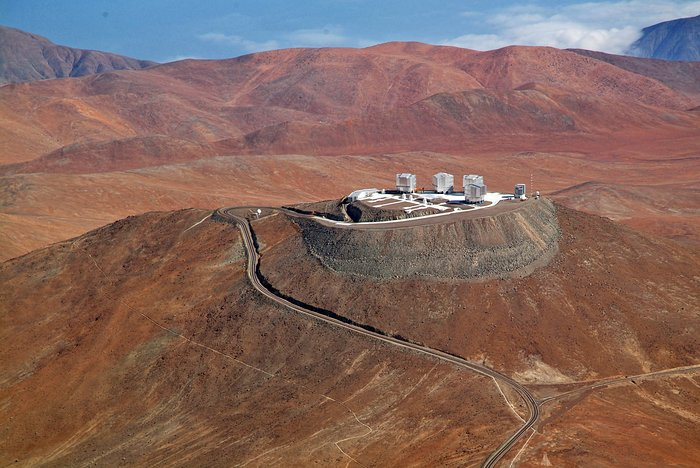
\includegraphics[width=0.7\textwidth]{Kap1/telescope.jpg}
\end{center}
\caption[short]{Vista aérea de la plataforma del ``ESO Very Large Telescope (VLT)", en la cima del Cerro Parnal, en el desierto chileno de Atacama. Créditos: J.L. Dauvergne  y G. Hüdepohl }
\label{fig:vvv_telescope}
\end{figure}

\par En este contexto, las estrellas variables de tipo RR Lyrae son una poderosa herramienta para obtener distancias a poblaciones de estrellas en la Vía Láctea, debido a que satisfacen una relación entre sus períodos y sus luminosidades absolutas que permite estimar distancias \cite{Shapley} \cite{Baade}. Sin embargo, a causa de la inmensa cantidad de información generada, la clasificación manual de estrellas se vuelve impracticable. Se requiere, por lo tanto, un método automatizado para identificar estrellas variables de tipo RR Lyrae de entre las $10^6-10^7$ estrellas variables que se espera encontrar en el área explorada \cite{jbc}. \\

\par Investigaciones recientes han mostrado que algoritmos de aprendizaje automatizado basados en ensambles de árboles tienen un excelente desempeño en este tipo de tareas, en tanto que otros métodos tradicionales como Support Vector Machines parecen no ser tan efectivos \cite{elorrieta} \cite{jbc}. El objetivo de esta tesina es intentar mejorar los resultados previos en el problema de detección de RR Lyrae en la VVV utilizando Support Vector Machines, así como comprender por qué métodos basados en ensambles de árboles aparentan funcionar mejor en este tipo de datos.  \\

\par Durante este trabajo se hizo uso de una amplia variedad de técnicas de aprendizaje automatizado, incluyendo diversos tipos de preprocesamiento, reducción de dimensionalidad y selección de variables, visualización de los datos y corrección de imbalance de clases. 

\section {Conceptos astronómicos}

\subsection{Estrellas RR Lyrae}

\par Una \textbf{estrella} es un objeto astronómico que consiste en una esfera luminosa de plasma, la cual mantiene su forma debido a su propia gravedad. Características como luminosidad, tamaño, evolución y duración de vida son definidas principalmente por su masa inicial. \\

\par Aquellas estrellas cuya luminosidad (magnitud aparente\footnote{Este valor indica la medida del brillo y cantidad de energía por segundo por metro cuadrado que se recibe de un objeto celeste por un observador en la Tierra. Como dicha cantidad recibida depende de la transmisión de la atmósfera en dichas bandas, las magnitudes aparentes se normalizan a un valor fuera de la atmósfera terrestre. La escala de magnitudes es una relación inversa logarítmica por la cual la estrella más brillante es la que tiene menor magnitud}) exhibe cambios periódicos o aleatorios se denominan \textbf{estrellas variables.} Las estrellas de tipo variable han jugado un rol crucial en la historia de la astronomía. El Catálogo General de Estrellas Variables \cite{catalogo} enumera más de 110 clases y subclases de estrellas variables. \\

\par Las estrellas variables pueden, en primera instancia, clasificarse en \textbf{variables intrínsecas} y \textbf{variables extrínsecas}, dependiendo del origen de la variabilidad observada. Si la causa de la variabilidad observada es inherente a la estrella, como es el caso de una estrella que periódicamente se expande y contrae, se le denomina intrínseca. Contrariamente, aquellas estrellas cuya variabilidad se debe a factores externos, como un compañero orbital que ocasionalmente la eclipsa, se denominan variables extrínsecas. \\

\par Probablemente el subgrupo más importante de las estrellas variables intrínsecas son las \textbf{estrellas pulsantes}, que varían en radio y luminosidad en el tiempo, expandiéndose y contrayéndose con períodos tan breves como minutos, o tan extensos como años, dependiendo del tamaño de la estrella. Para una revisión moderna de la fenomenología de estrellas pulsantes, puede remitirse a \cite{fisica}. \\

\par  Dentro de las estrellas pulsantes, se encuentran las subclases \textbf{RR Lyrae} y \textbf{Cepheids}, las cuales satisfacen una relación entre sus períodos y sus luminosidades absolutas que las convierte en invaluables herramientas para una de las tareas más complejas en astronomía: estimar distancias \cite{Shapley} \cite{Baade}. \\

\par Las estrellas de tipo \textbf{RR Lyrae} (en adelante, RRL) tienen períodos de entre 0.2 y 1.2 días \cite{smith}, y tienen una edad de aproximadamente 14 Gyr\footnote{1 gigayear (Gyr) = $10^9$ años}. Son consideradas excelentes candelas estándar, especialmente importantes a la hora de explorar distancias y propiedades de viejas problaciones estelares. Basándose en relevamientos recientes, se estima que hay alrededor de 140000 estrellas RRL en nuestra galaxia \cite{ogle} \cite{gaia} \\

\par En base a sus curvas de luz, las RRL fueron originalmente separadas en subtipos a, b y c \cite{bailey}, aunque posteriores trabajos unificaron los dos primeros subtipos en uno solo, RRab, dado que son fundamentalmente distintos del tercero, RRc \cite{schwarzschild}. Adicionales subtipos, extremadamente raros, fueron añadidos posteriormente. \\

\subsection{El relevamiento VVV}

\par ``Vista Variables in the Via Lactea (VVV) ESO Public Survey'' es un relevamiento fotométrico (terrestre) del bulbo galáctico y parte del disco interno de la Vía Láctea, que se llevó a cabo utilizando el telescopio VISTA en Parnal, Chile.  Uno de los objetivos principales de la VVV es adquirir un mayor entendimiento del origen, estructura y evolución de la Vía Láctea. Para una descripción detallada de la VVV puede consultarse \cite{vvv}, en tanto que un artículo más reciente con énfasis en variabilidad puede consultarse en \cite{vvv_actual} \\

\par El VVV, así como su sucesor el ``VVV Survey eXtended'', i.e. VVVX, persiguen el objetivo de producir un atlas profundo de una gran parte del Bulbo de la Vía Láctea, así como de una fracción del Disco Galáctico interno. Este mapa se produjo mediante un monitoreo sistemático de estas regiones, habiéndose completado 1929 horas de observación durante cinco años, comenzando en 2010. \\

\par Dentro del barrido total del relevamiento, es de interés astronómico la generación de catálogos de cualquier tipo de objeto, esperándose identificar no sólo estrellas variables, sino planetas, asteroides y otros fenómenos. En la figura \ref{fig:vvv_objects} se ilustra el número de fenómenos estimado.

\begin{figure}[h]
\begin{center}
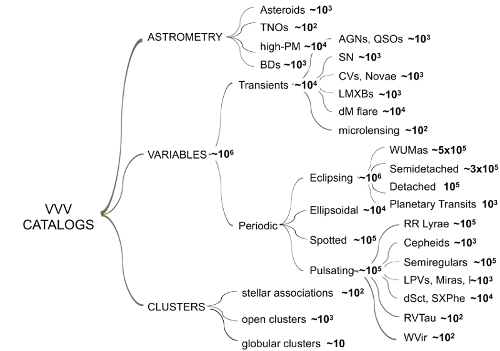
\includegraphics[width=0.7\textwidth]{Kap1/vvv_objects.png}
\end{center}
\caption[short]{Número esperado de fenómenos astrofísicos que espera detectar VVV en sus catálogos. Minniti et. al. 2010.}
\label{fig:vvv_objects}
\end{figure}

\par Los datos del VVV se presentan en una unidad llamada baldosa (tile, en inglés), una zona rectangular del cielo de $1.501 deg^2$ relevada a través del tiempo. Se requirieron 196 tiles para mapear el área del Bulbo, así como 152 tiles para el Disco. Cada tile se compone de varias imágenes en alta resolución para diferentes tipos de filtros (bandas anchas) de frecuencias lumínicas en el infrarrojo cercano (cinco en total). Asimismo, por cada imagen existe una base de datos con los valores de posición, magnitud y color de las fuentes de luz presentes en la imagen, llamada “catálogo fotométrico”. En el caso del VVV, la totalidad de las baldosas que constituyeron el relevamiento puede apreciarse en la figura \ref{fig:vvv_tiles} \\

\begin{figure}[h]
\begin{center}
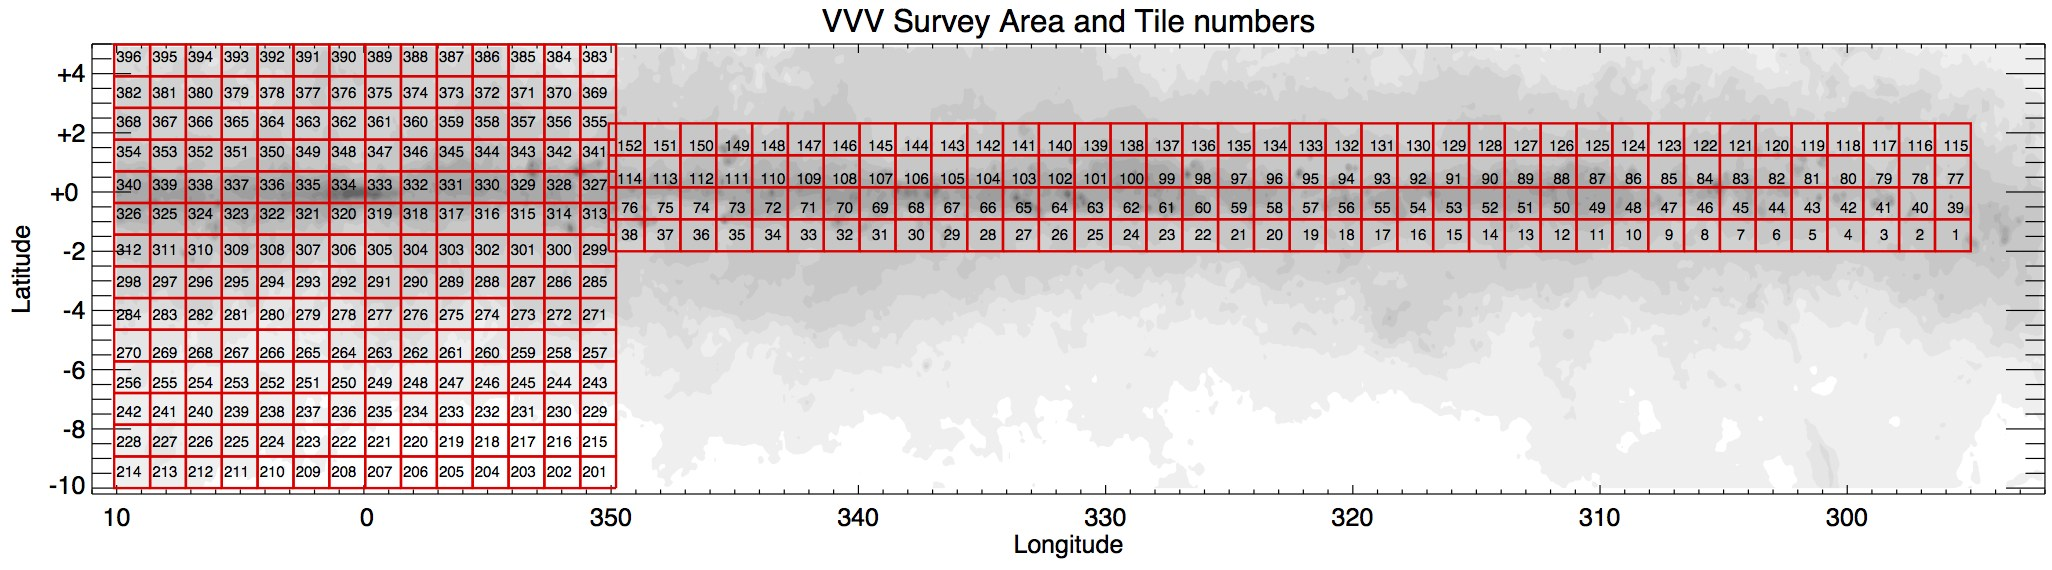
\includegraphics[width=\textwidth]{Kap1/vvv_tiles.jpg}
\end{center}
\caption[short]{Área del relevamiento VVV, en coordenadas galácticas. En escala de grises se puede apreciar la densidad estelar del área relevada. ~\protect\cite{Skrutskie_2006}}
\label{fig:vvv_tiles}
\end{figure}

\par La identificación de aquellas fuentes de luz que corresponden a estrellas RRL es de particular interés para VVV, dado que determinar distancias es vital para cumplir uno de sus objetivos primordiales: mapear el Bulbo Galáctico. Más aún, la existencia de trabajos previos \cite{gran1} \cite{gran2} que identifican algunos cientos de fuentes de luz como RRL dentro del área mapeada por la VVV, implica que se cuenta con un conjunto de datos que puede ser utilizado para entrenar y testear clasificadores de aprendizaje automatizado. 

\subsection{Extracción de features}

\par En esta tesina se hace un uso extensivo de los datos producidos en \cite{jbc}. Por cada tile en un subconjunto de tiles del relevamiento, se generó un dataset numérico, donde cada fila corresponde a una estrella, descripta por 62 features (atributos) numéricas. En esta sección se explicará, a alto nivel, cómo se obtuvieron dichas features a partir de las mediciones de fotometría del infrarrojo cercano producidas por VVV. \\

\par Durante el relevamiento VVV se generaron enormes volúmenes de datos (1.4 TB/noche). El pipeline de VVV \cite{emerson} brinda, por cada imagen generada, una base de datos de archivos con los valores de posición, magnitud y color de las fuentes de luz presentes, llamada \textbf{catálogo fotométrico}. Aunque existen varios tipos de catálogos,  sólo dos son utilizados en este trabajo:

\begin{itemize}
\item En primer lugar, el catálogo \textbf{Pawprint Stack} contiene lecturas de los sensores infrarrojos de la cámara VIR-CAM del telescopio VISTA, correspondientes a la observación de un tile en una fecha dada (también llamado época). 
\item En segundo lugar, el catálogo \textbf{Band Merge} se utiliza para tener una lista confiable de estrellas en un cierto tile, dado que ciertas fuentes de luz pueden no estar presentes entre distintos Pawprint Stacks debido a condiciones meteorológicas o problemas en los instrumentos de medición.
\end{itemize}

\par Para determinar la variación en magnitud de cada estrella presente en cada Band Merge, fue necesario identificar todas sus ocurrencias en diferentes Pawprint Stacks. De esta forma, se puede formar una serie temporal de observaciones de la estrella en cuestión, haciendo uso de técnicas de cross-matching \cite{cross}. El resultado son series temporales como la que se puede apreciar en la figura \ref{fig:curva_de_luz}. Nótese que el tiempo de muestreo puede ser muy irregular, por lo que se presupone que es aleatorio. \\


\begin{figure}[h]
\begin{center}
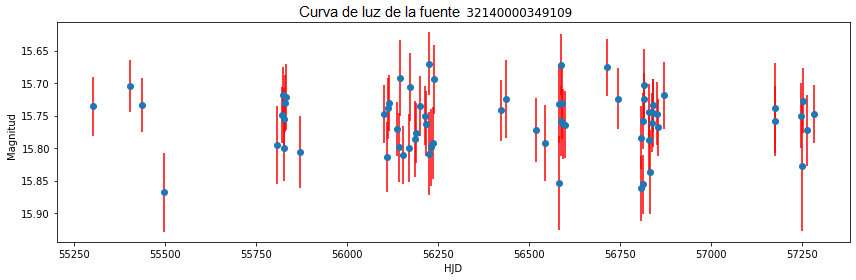
\includegraphics[width=\textwidth]{Kap1/light_curve.png}
\end{center}
\caption[short]{Curva de luz de una de las estrellas relevadas por VVV. El eje $x$ muestra el tiempo expresado en días heliocéntricos medios (HJD), en tanto que el eje $y$ muestra la magnitud aparente observada. Cada punto azul corresponde a una observación en un cierto Pawprint Stack, mientras que las líneas rojas indican el error asociado a cada medición. Imagen tomada de la documentación de Carpyncho, \url{https://carpyncho-py.readthedocs.io/} }
\label{fig:curva_de_luz}
\end{figure}

\par Habiéndose obtenido las series temporales de cada estrella, el siguiente paso fue estimar su período. Se utiliza el método de Fast Lomb-Scargle \cite{Lomb:1976wy} \cite{scargle} \cite{VanderPlas_2018} para recuperar cada período, el cual consiste en ajustar una función sinusoidal a los datos muestreados. \\

\par A partir de las curvas de luz y el período estimado, se extrajeron 49 atributos (o características) numéricas utilizando la herramienta \textit{Feets} \cite{cabral2018fats}. Estos atributos se refieren al período, variación de magnitud y morfología de las curvas de luz. Una descripción de cada atributo puede consultarse en el apéndice \ref{AnexoA}. \\

\par Una contribución original de \cite{jbc} fue la inclusión de atributos que describen las temperaturas o colores intrínsecos de cada estrella.  Dado que la presencia de polvo interestelar ocasiona un fenómeno denominado extinción, que provoca un enrojecimiento de los colores, fue necesario realizar una corrección utilizando mapas de extinción \cite{mcwilliam2011rr}. Como resultado final, se extrajeron 13 atributos numéricos describiendo el color de cada estrella. Nuevamente, la lista completa de atributos de color, junto con sus descripciones está disponible en el apéndice \ref{AnexoA}.

\subsection{Descripción de los datos}
\label{tiles_description}
En esta sección se describirán en detalle los datasets generados en \cite{jbc}, que pueden ser accedidos por el público a través de la librería Python \textbf{Carpyncho}\cite{carpynchoToolkit}.\\

Cada dataset generado corresponde a un cierto tile de la VVV. Cada fila de un dado dataset se corresponde a una cierta estrella variable, descripta por 62 features numéricas tal y como se describió en la sección anterior. La siguiente tabla resume los datos liberados por Carpyncho:

\begin{table}[h]
\centering
\begin{tabular}{|l|l|l|l|l|l|}
\hline
\textbf{Tile}  & \textbf{Épocas} & \textbf{Tamaño} & \textbf{RRL} & \textbf{Unknown} & \textbf{RRL / Tamaño} \\ \hline
b206           & 73              & 157825          & 47           & 157778           & 0.03\%                \\ \hline
b214           & 74              & 149557          & 34           & 149523           & 0.02\%                \\ \hline
b216           & 73              & 168996          & 43           & 168953           & 0.03\%                \\ \hline
b220           & 73              & 209798          & 65           & 209733           & 0.03\%                \\ \hline
b228           & 73              & 199853          & 28           & 199825           & 0.01\%                \\ \hline
b234           & 73              & 293013          & 126          & 292887           & 0.04\%                \\ \hline
b247           & 73              & 406386          & 192          & 406194           & 0.05\%                \\ \hline
b248           & 74              & 417839          & 218          & 417621           & 0.05\%                \\ \hline
b261           & 74              & 555693          & 252          & 555441           & 0.05\%                \\ \hline
b262           & 74              & 573873          & 314          & 573559           & 0.06\%                \\ \hline
b263           & 94              & 568110          & 317          & 567793           & 0.06\%                \\ \hline
b264           & 94              & 595234          & 307          & 594927           & 0.05\%                \\ \hline
b277           & 73              & 718567          & 429          & 718138           & 0.06\%                \\ \hline
b278           & 74              & 742153          & 436          & 741717           & 0.06\%                \\ \hline
b360           & 74              & 939110          & 669          & 938441           & 0.07\%                \\ \hline
b396           & 73              & 486639          & 15           & 486624           & 0.00\%                \\ \hline
\textbf{Total} & 1216            & 7182646         & 3492         & 7179154          & 0.05\%                \\ \hline
\end{tabular}
\end{table}

\par Como se puede observar, algunas de las estrellas variables de cada dataset están identificadas como RRL. Estas etiquetas provienen de realizar cross-matching con catálogos de estrellas variables de otros relevamientos con zonas de observación superpuestas a la VVV: \textit{OGLE-III} \cite{Udalski}, \textit{OGLE-IV} \cite{Udalski2} y VizieR \cite{vizier}. \\

\par En todos los experimentos de clasificación de este trabajo, se consideró como clase positiva a aquellas estrellas etiquetadas como RRL, siendo el resto la clase negativa. Es importante mencionar que nuestras clases positivas y negativas no son completamente certeras, dado que no han sido validadas con una inspección manual de cada fuente. Es posible que ciertas estrellas etiquetadas como RRL en realidad no lo sean y viceversa. Esto es especialmente válido en tiles como \textit{b396}, para las cuales hay pocas RRL previamente clasificadas en relevamientos anteriores. \\

\par Para la mayoría de los experimentos en este trabajo, se utilizó un subconjunto de tiles (\textit{b234}, \textit{b261}, \textit{b278} y \textit{b360} ) correspondiente a áreas del Bulbo que resultan de particular interés:

\begin{itemize}
\item Hay una buena densidad de RRL, pues las zonas se superponen bien con relevamientos anteriores. Por lo tanto, es probable que haya menos RRLs etiquetadas como no-RRL.

\item \textit{b278} es de particular interés pues contiene la llamada ventana de Baade, una zona con poco polvo intergaláctico en la línea visual de la tierra al núcleo galáctico \cite{Baade}. Esta zona ha sido históricamente utilizada para estudiar RRL.

\end{itemize}

\section {Aprendizaje automatizado}

Esta sección introducirá brevemente algunos conceptos básicos de aprendizaje automatizado, y está fuertemente basada en los capítulos introductorios de \cite{mitchell} y \cite{slearning}.

\subsection{Definición y tipos de aprendizaje}

El campo del \textbf{aprendizaje automatizado} consiste en el estudio de algoritmos que mejoran automáticamente su rendimiento gracias a la experiencia. Formalmente, Tom Mitchell en su libro \textit{ ``Machine Learning''} \cite{mitchell} define aprendizaje automatizado como sigue:

\begin{quotation}
Se dice que un programa de computadora aprende de la experiencia $E$ respecto a una tarea $T$ y una medida de desempeño $P$ , si el desempeño medido con $P$ en una tarea $T$ , mejora con la experiencia $E$.
\end{quotation}

Dada una muestra de datos, los algoritmos de aprendizaje automatizado construyen un modelo con el objeto de realizar predicciones o tomar decisiones \textit{sin haber sido expresamente programados para hacerlo}. Tales algoritmos pueden ser aplicados a un amplio rango de tareas, tales como aprender a conducir un vehículo autónomo \cite{Pomerleau-1989-15721}, aprender a jugar backgammon a nivel profesional \cite{Tesauro1995} o clasificar estructuras astronómicas \cite{clasify_astronomy}.  \\

Tradicionalmente, las distintas tareas a llevar a cabo por algoritmos de aprendizaje automatizado se dividen en tres paradigmas \cite{ai}:

\begin{itemize}
\item \textbf{Aprendizaje supervisado}: Consiste en aprender una función $f : I \mapsto O$, basándose en un conjunto de ejemplos $T \subset I \times O$ . En otras palabras, el algoritmo de aprendizaje automatizado intenta inferir una función a partir de un conjunto de entradas de ejemplo, etiquetadas con su valor de salida. Si el conjunto $O$ es discreto, se trata de una tarea de \textbf{clasificación}; en tanto que si es continuo, se trata de una tarea de \textbf{regresión}.
\item \textbf{Aprendizaje no supervisado}: En aprendizaje no supervisado, sólo hay entradas pero no salidas, por lo que el objetivo es aprender patrones y relaciones en conjuntos de datos no etiquetados.

\item \textbf{Aprendizaje por refuerzo (Reinforcement learning)}: Consiste en aprender a tomar decisiones en un ambiente dinámico, con el objeto de maximizar una cierta noción de recompensa acumulada. 
\end{itemize}

En este trabajo nos enfocaremos en técnicas de aprendizaje automatizado supervisado, dado que se desea abordar la tarea de clasificar estrellas variables en RRL o no-RRL. 

\subsection{Medidas de performance}
\label{ml_intro_test}
Como se mencionó anteriormente, el aprendizaje supervisado consiste en aproximar una función $f : I \mapsto O$. Durante una primera fase de \textbf{entrenamiento}, un conjunto de $n$ ejemplos $x_i \in I, \ i=1,\ldots,n$ junto con sus salidas asociadas $y_i \in O$ es utilizado para enseñar al modelo cómo estimar $f$. \\

Existe una amplia variedad de métodos de aprendizaje supervisado, y ninguno domina a todos los demás en todo conjunto de datos. El desempeño de cada método es altamente dependiente del problema a abordar, por lo que resulta de suma importancia decidir qué método produce los mejores resultados para un dado conjunto de datos. \\

Para evaluar el desempeño de un método, se necesita alguna forma de medir cuán bien el valor predicho por el método para una dada observación, se condice con la verdadera respuesta para esa observación. Sea $\hat{f}$ la estimación de $f$ obtenida por el método de aprendizaje supervisado en estudio:

\begin{itemize}

\item  En problemas de regresión, la métrica más comúnmente utilizada es el \textit{error cuadrático medio}:

\begin{center}
$MSE = \sum_{i=1}^{n} ( y_i - \hat{f}(x_i) )^2 $
\end{center}

\item En problemas de clasificación, podemos calcular la proporción de errores realizados:

\begin{center}
$Error \ Rate = \frac{1}{n} \sum_{i=1}^{n} I( y_i , \hat{f}(x_i) ) $
\end{center}

Donde:
\begin{center}
$
I(y_i,\hat{y_i}) =
\left\{
	\begin{array}{ll}
		0  & \mbox{si } y_i = \hat{y_i} \\
		1 & \mbox{si } y_i \neq \hat{y_i}
	\end{array}
\right.
$
\end{center}

\end{itemize}

Ambas métricas fueron definidas sobre los datos de entrenamiento. Sin embargo, en general, no nos importa cuán bien el método funciona en los datos de entrenamiento. Estamos interesados en las métricas obtenidas al aplicar nuestro modelo ya entrenado a un conjunto de datos de test, que no hayan sido previamente utilizados en la fase de entrenamiento. \\

Esto nos lleva a la distinción entre \textit{training MSE} y \textit{training Error Rate}, en contraposición a \textit{test MSE} y \textit{test Error Rate}. Usualmente, se reserva una porción de los datos disponibles para ser utilizada como \textbf{conjunto de test}. Estos datos no son utilizados en la fase de entrenamiento, y son utilizados para calcular métricas como \textit{test Error Rate} una vez terminada la fase de entrenamiento. Tales métricas proveen una noción de cuán bien el clasificador funcionará en datos no antes vistos. Una alternativa para obtener tales métricas sin necesidad de tener un conjunto separado de test es utilizar \textbf{cross validation} \cite{cross_validation}. \\

En este trabajo estamos particularmente interesados en problemas de \textbf{clasificación binaria}, es decir, problemas de aprendizaje automatizado supervisado en los cuales el conjunto de etiquetas contiene solo dos elementos, o clases, a menudo llamados clase positiva y negativa. En problemas de clasificación binaria, cada elemento se puede clasificar en una de las siguientes cuatro categorías: \\

\begin{table}[h!]
\begin{tabular}{l|l|l|}
\cline{2-3}
                                                    & \textbf{Clase predicha: Negativa} & \textbf{Clase predicha: Positiva} \\ \hline
\multicolumn{1}{|l|}{\textbf{Clase real: Negativa}} & Verdadero negativo (TN)           & Falso positivo (FP)               \\ \hline
\multicolumn{1}{|l|}{\textbf{Clase real: Positiva}} & Falso negativo (FN)               & Verdadero positivo (TP)           \\ \hline
\end{tabular}
\end{table}

Los falsos positivos son aquellos elementos de clase negativa, clasificados incorrectamente con etiqueta positiva. Similarmente, los falsos negativos son aquellos elementos con etiqueta positiva, clasificados como negativos. Los verdaderos positivos (negativos), son aquellos elementos positivos (negativos), que fueron clasificados correctamente. \\

Dado un cierto conjunto de datos etiquetados, la performance de un clasificador binario puede visualizarse al calcular una \textbf{matriz de confusión}. La matriz de confusión mostrará la suma de elementos de cada una de las cuatro categorías explicadas. En particular, podemos reescribir la métrica Error Rate como: \\

\begin{center}
$ Error Rate = \frac{FP + FN}{FP + FN + TP + TN} $
\end{center}

Equivalentemente, es usual analizar la \textbf{tasa de aciertos}:

\begin{center}
$ Acc = \frac{TP + TN}{FP + FN + TP + TN} $
\end{center}

\subsection{Problemas desbalanceados}
\label{imbalance}

A la hora de estudiar problemas de clasificación, es importante tener en cuenta la proporción de datos de cada clase. Un \textbf{problema de clasificación desbalanceado} es aquel en el cual la cantidad de elementos de cada clase no es proporcional. Ciertas aplicaciones como diagnóstico médico o detección de transacciones fraudulentas con tarjeta de crédito presentan datasets con un número muy pequeño de instancias positivas\footnote{En problemas de clasificación binaria, usualmente se considera clase positiva a la clase minoritaria, en tanto que la clase mayoritaria es la negativa}, que son sin embargo cruciales de clasificar correctamente \cite{imbalanced_svm}. \\

Si se utilizan datasets imbalanceados para entrenar y testear, es inadecuado utilizar métricas de desempeño basadas en clasificar la \textit{mayor cantidad} de elementos de forma correcta, como $Acc$. La hipótesis mas sencilla, clasificar todas las instancias como pertenecientes a la clase mayoritaria, a menudo maximiza tales métricas. \\

Un primer paso a la hora de trabajar con datos desbalanceados es, entonces, utilizar métricas que no son sensitivas al imbalance de clases. En clasificación binaria, las siguientes métricas son de interés:

\begin{itemize}
\item \textbf{Precisión}: La proporción de instancias clasificadas como positivas, que realmente lo son:
\begin{center}
$ Precision =  \frac{TP}{TP + FP}$
\end{center}

\item \textbf{Recall}: La proporción de instancias positivas que son detectadas por el clasificador.
\begin{center}
$ Recall =  \frac{TP}{TP + FN}$
\end{center}

\end{itemize}

A menudo, muchos métodos de aprendizaje automatizado para clasificación binaria producen un puntaje\footnote{Se utiliza el término puntaje (del inglés \textit{score}), dado que no se utilizará un enfoque probabilístico.} en $[0,1]$ para cada instancia a clasificar. Puntajes cercanos a 0 indican que el clasificador tiene mayor certeza de que una cierta entrada pertenece a la clase negativa, en tanto que valores cercanos a 1 indican pertenencia a la clase positiva. \\

En tal escenario, resulta necesaria la elección de un umbral $t \in [0,1]$, de forma tal que sólo instancias cuyos puntajes son mayores a $t$ sean clasificadas como positivas, siendo las demás negativas. En consecuencia, resulta importante determinar un $t$ adecuado para el dominio de aplicación en estudio, dado que distintos valores de $t$ tendrán un impacto directo en la matriz de confusión producida. \\

Valores altos de $t$ tenderán a producir clasificadores con mayor precisión y menor recall, en tanto que valores pequeños de $t$ tenderán a clasificadores con mayor recall y menor precisión. Una forma gráfica de analizar esta correspondencia es a través de la curva de precision-recall del clasificador, como la de la figura \ref{fig:prc}, en la cuál se grafica la precisión y el recall obtenidos para un rango de valores de $t$. \\

\begin{figure}[h]
\begin{center}
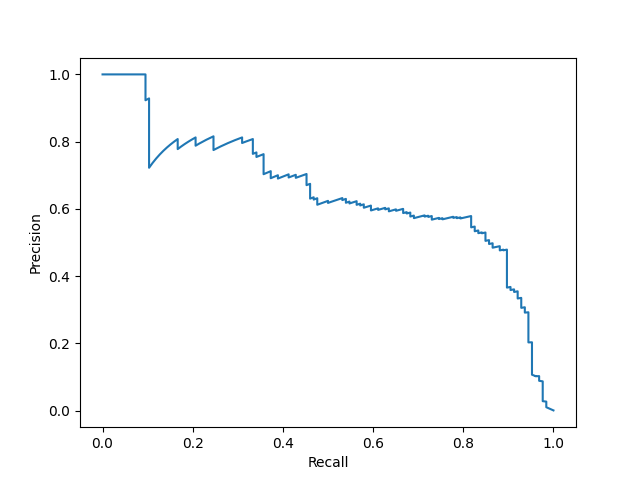
\includegraphics[width=.6\textwidth]{Kap1/PRc.png}
\end{center}
\caption[short]{Ejemplo de una curva de precision-recall. Cada punto de la curva corresponde a la precisión y el recall obtenidos para un cierto valor de $t$. }
\label{fig:prc}
\end{figure}

Si se está abordando un problema desbalanceado, una forma determinar si un clasificador tiene mejor performance que otro es comparar sus curvas de precision-recall en el dataset de test. Dado que las curvas de precision-recall tienden a ser bastante ruidosas en áreas de bajo recall, en este trabajo se utilizó en repetidas ocasiones el área bajo la curva de precision-recall restringida al dominio [0.35,1] para obtener una medida de performance numérica, a la que llamaremos R-AUPRC (del inglés Robust Area Under the Precision Recall Curve, área debajo de la curva de precision-recall robusta).\\


R-AUPRC resulta útil cuando se desea comparar decenas o cientos de curvas a la vez, siendo imposible su inspección visual y prefiriéndose aquel modelo que maximiza el R-AUPRC. Otra métrica alternativa es utilizar la precisión del clasificador a un cierto valor fijo de recall. \\

Además de utilizar métricas adecuadas para evaluar el desempeño, otras técnicas para trabajar con datos desbalanceados son:

\begin{itemize}
\item Corregir manualmente el imbalance de clases en los datos. Una posibilidad es eliminar datos de la clase mayoritaria aleatoriamente (\textbf{undersampling}) \cite{nathalie} hasta alcanzar el balance deseado. Una segunda posibilidad es generar nuevas instancias de la clase minoritaria (\textbf{oversampling}). \cite{he}
\item Forzar a que el clasificador preste más atención a la clase minoritaria \cite{imbalanced_svm}. Por ejemplo, como se verá en secciones posteriores, para ciertos métodos de aprendizaje automatizado como Support Vector Machines es posible asociar un peso (\textit{class\_weight}) a cada clase, de tal forma que el clasificador será menos permisivo a la hora de clasificar incorrectamente clases con alto peso.
\end{itemize}

\subsection{Árboles de decisión}
En esta sección se presentará brevemente uno de los métodos de aprendizaje automatizado supervisado para clasificación más ampliamente utilizado: Árboles de Decisión\cite{mitchell}. \\

Los árboles de decisión están formados por dos tipos de elementos: nodos y ramas. En primer lugar, veamos cómo se usa un árbol de decisión ya construido. En la figura \ref{fig:tree} podemos ver un ejemplo de un árbol de decisión que intenta predecir si un pasajero sobreviviría o no al hundimiento del Titanic.  \\

Supongamos que cada persona está descripta por tres atributos numéricos: edad, género y número de familiares en el barco (sibsp). Para clasificar una nueva instancia, se desciende por el árbol comenzando por la raíz. En cada nodo, se realiza una comparación sobre un atributo de la instancia a clasificar, y se desciende por una de las dos ramas del árbol de acuerdo al resultado. \\

\begin{figure}[h!]
\begin{center}
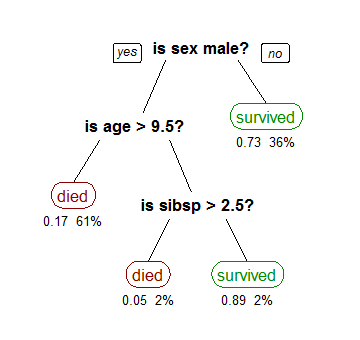
\includegraphics[width=.44\textwidth]{Kap1/tree.png}
\end{center}
\caption[short]{Árbol de decisión construido sobre el dataset \textit{Titanic}. Los árboles de decisión se dibujan invertidos, con la raíz en la parte superior. Créditos: Wikipedia. }
\label{fig:tree}
\end{figure}

El proceso continúa hasta llegar a un nodo que no posee más subdivisiones, tales nodos son llamados \textbf{hojas} e indicarán la clase final que con la cual el clasificador etiquetará la nueva instancia. \\

Ahora que ya se ha discutido cómo utilizar un árbol de decisión existente, veamos cómo se crea un nuevo árbol a partir de un conjunto de entrenamiento. Un algoritmo greedy para crecer un árbol de decisión consiste en crear cada nodo recursivamente, comenzando desde la raíz. Naturalmente, se debe decidir qué atributo utilizar en cada nodo no hoja para realizar la división; así como el valor de corte que se utilizará (\textit{split} en inglés). A la hora de crear un nodo, se considerará para cada atributo un cierto número de valores de corte, y se elegirá aquel que minimice una cierta métrica de costo sobre los datos de entrenamiento. \\

Distintas métricas pueden utilizarse para decidir cuál es el mejor split, intentando incentivar la homogeneidad de la variable objetivo en los subconjuntos producidos. Dos métricas muy populares son \textit{Gini Impurity} e \textit{Information Gain} \cite{ginigain}.\\

Un aspecto a considerar es cuándo detener este proceso de crecimiento. Es posible que árboles extremadamente complejos conduzcan a \textbf{sobreajuste} (overfitting en inglés), un fenómeno en el cual un método de aprendizaje automatizado se ajusta demasiado bien a los datos de entrenamiento, aprendiendo detalles y ruido presentes; y por lo tanto perdiendo desempeño al clasificar instancias nuevas. Por lo tanto, puede ser valioso detener el crecimiento del árbol prematuramente.%, o bien \textit{podarlo} (eliminar algunos nodos) posteriormente. 

\subsection{Random Forests}

En esta sección se introducirá brevemente uno de los dos métodos de clasificación utilizados en este trabajo: Random Forests \cite{rf}. Random Forest es un método \textbf{ensamble}, más específicamente de tipo \textbf{bagging}. \\

Los métodos ensamble consisten en utilizar \textit{múltiples} algoritmos de aprendizaje para mejorar el desempeño que cada uno de ellos tiene individualmente. En concreto, los métodos de bagging \cite{bagging} se basan en generar múltiples versiones de un mismo predictor, perturbando los datos de entrenamiento que se le suministran a cada uno, y combinando sus resultados para formar un clasificador más potente. \\

En particular, Random Forest es un ensamble donde los predictores individuales son árboles de decisión. Un Random Forest formado por $n$ árboles de decisión, se construye de la siguiente forma:

\begin{enumerate}
\item \textbf{Crear un bootstrap del dataset de entrenamiento por cada árbol a construir}: En lugar de utilizar el dataset de entrenamiento completo para entrenar cada árbol de decisión, se calculará un bootstrap (sampleo aleatorio con reemplazo) por cada árbol de decisión a entrenar. 
\item \textbf{Entrenar cada árbol de decisión}: Se entrena cada árbol de decisión utilizando uno de los bootstraps generados en el paso anterior. Para añadir aún más aleatoriedad, se considera únicamente un subconjunto aleatorio de atributos en cada nodo a la hora de elegir el mejor split.
\end{enumerate}

Una de las principales desventajas de los árboles de decisión es que tienen tendencia a sobreajustar los datos de entrenamiento. La aleatoriedad involucrada en el primer paso, implica que si bien cada árbol puede sobreajustar sus datos de entrenamiento; el Random Forest completo no sobreajustará ningún subconjunto de datos en especial. \\

Los métodos ensamble funcionan mejor si hay una cierta decorrelación, o variedad, en los modelos individuales. La aleatoriedad involucrada en el segundo paso también contribuye a esta decorrelación, evitando que ciertos atributos con alto poder predictivo sean incluidos en todos los árboles. \\

Una vez que el random forest ha sido construido, realizar predicciones para nuevas instancias es muy sencillo. Se evalúa la entrada en cuestión en cada uno de los árboles, obteniendo $n$ predicciones que se combinan para formar la predicción final del random forest. En problemas de clasificación, cada predicción puede considerarse un voto, y la predicción más votada será la predicción del random forest.\\

Random Forest es un método muy flexible y poderoso, y es cotidianamente utilizado en aplicaciones industriales. Una de sus principales ventajas es su facilidad de uso, dado que no se requiere la optimización de hiperparámetros complejos y brinda generalmente buenos resultados.

\subsection{Support Vector Machines}

\label{trick}

En esta sección se presentará el segundo método de aprendizaje automatizado supervisado para clasificación binaria que se utilizará en este trabajo: Support Vector Machines (SVM) \cite{svm2} \cite{svm}  \\

Una tarea de clasificación binaria puede ser vista como la tarea de separar las clases en el espacio de atributos. En la figura \ref{fig:sv1} podemos ver un ejemplo en el cual se decide utilizar un hiperplano para realizar dicha separación. Como se puede ver hay infinitos separadores lineales para este ejemplo. \\

\begin{figure}[h!]
\begin{center}
  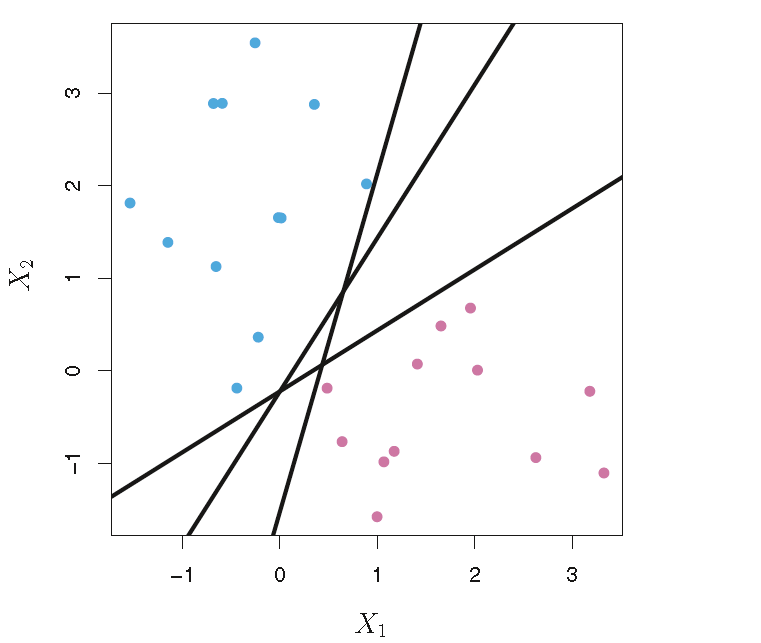
\includegraphics[width=0.56\textwidth]{Kap1/svm1.png} 
\end{center}
\caption{ En esta imagen podemos ver un ejemplo de clasificación binaria utilizando un separador lineal. Se ilustra la existencia de múltiples separadores lineales que podrían ser utilizados. Créditos: Drew Wilimitis, \url{towardsdatascience.com}.}
\label{fig:sv1}
\end{figure}

Las SVM buscan elegir el hiperplano que separe ambas clases maximizando el margen entre ambas clases, donde el margen se define como la mínima distancia entre un punto de training y el hiperplano separador. Esta situación se ilustra en la figura \ref{fig:svm_3}. \\

\begin{figure}[h!]
\begin{center}
  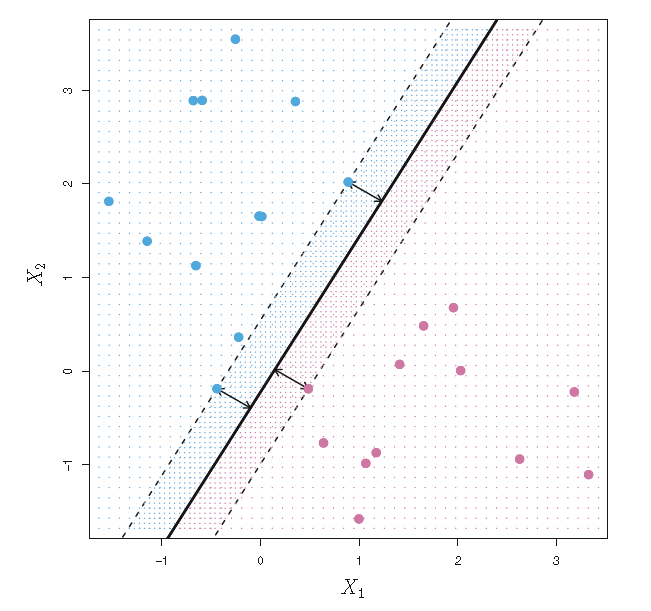
\includegraphics[width=0.56\textwidth]{Kap1/svm3.png} 
  \end{center}
 \caption{En esta imagen se ilustra el hiperplano escogido por SVM. Aquellos puntos que están a la menor distancia del hiperplano separador se denominan vectores soporte. SVM escoge el hiperplano que maximiza la separación entre ambas clases. Créditos: Drew Wilimitis, \url{towardsdatascience.com}}
\label{fig:svm_3}
\end{figure}


Un problema inmediato a considerar es que la frontera que separa las clases puede estar determinada por una superficie no lineal. Esto puede solucionarse mediante el uso de una función kernel, que mapea los datos a algún espacio de mayor dimensionalidad donde la frontera que separa las clases será, potencialmente, lineal. Esta situación es ilustrada en la figura \ref{fig:svm_4}\\

\begin{figure}[h!]
\begin{center}
  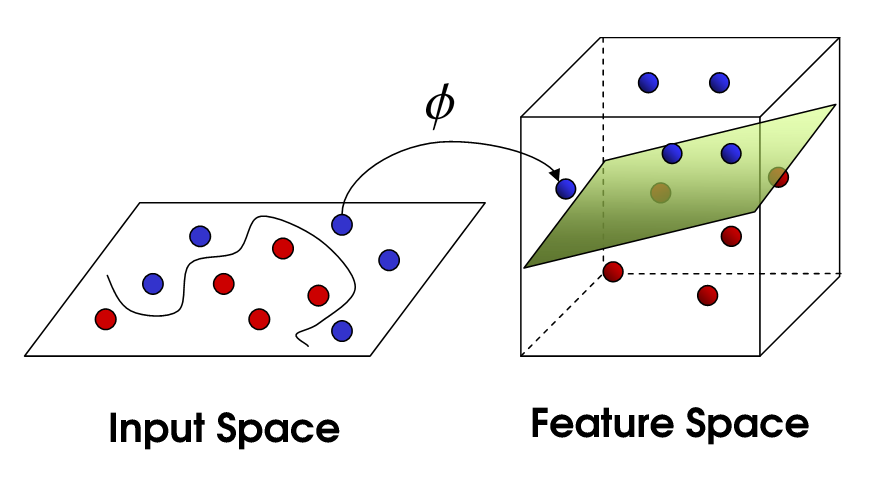
\includegraphics[width=0.7\textwidth]{Kap1/svm5.png} 
  \end{center}
 \caption{ Utilización de una función kernel para mapear puntos que no son linealmente separables a un espacio de mayor dimensionalidad, donde pueden ser separados por un hiperplano. Créditos: Drew Wilimitis, \url{towardsdatascience.com} }
\label{fig:svm_4}
\end{figure}

Matemáticamente, dado un conjunto de entrenamiento $\{ (x_i,y_i), \ i=1 \ldots l, \ x_i \in R^n \ , y_i \in \{1,-1\} \}$, SVM requiere solucionar el siguiente problema de optimización:

\begin{center}
$\begin{aligned}
\min_{w,b,\xi} \quad & \frac{1}{2}w^{t}w+C\sum_{i=1}^{l}{\xi_{i}}\\
\textrm{s.t.} \quad & y_{i}(w^T\phi(x_{i})+b) \geq 1 - \xi_{i}\\
  &\xi\geq0    \\
\end{aligned}
$
\end{center}

Nótese que los vectores de entrenamiento $x_i$ son mapeados a un espacio de mayor dimensionalidad (quizás infinita) a través de la función $\phi$. SVM encuentra un hiperplano que separa ambas clases con el máximo margen posible. \\

$C>0$ es un hiperparámetro de penalidad que regula cuánto error se permite, introduciendo  variables slack $\xi_i$ que permiten a algunos vectores estar del lado equivocado de la frontera. Esta situación es ilustrada en la figura \ref{fig:svm_5}\\


\begin{figure}[h!]
\begin{center}
  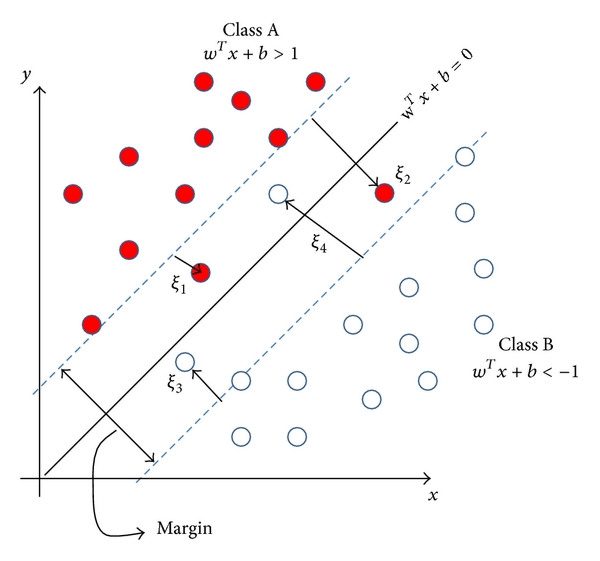
\includegraphics[width=0.4\textwidth]{Kap1/slack.jpg} 
  \end{center}
 \caption{ Utilización de variables slack que permiten a algunos puntos de entrenamiento estar dentro del margen, e incluso del lado equivocado del hiperplano. El parámetro C permite regular cuán permisivo es el modelo a la hora de permitir errores de clasificación. Imagen tomada de \textit{Hybrid Model Based on Genetic Algorithms and SVM Applied to Variable Selection within Fruit Juice Classification}, Carlos Fernandez-Lozano et al. }
\label{fig:svm_5}
\end{figure}

$K(x_i,x_j) = \phi(x_i)^T \phi(x_j)$ es llamada \textbf{función kernel}. Algunas de las funciones kernel más populares son:

\begin{itemize}
\item \textbf{Lineal}: $K(x_i,x_j) = x_i^T x_j$
\item \textbf{Polinomial}: $K(x_i,x_j)= (\gamma x_i^T x_j + r)^d , \ \gamma > 0$
\item \textbf{Radial Basis Function (RBF)}: $K(x_i,x_j)= exp (-\gamma\left\| x_i - x_j \right\|^2  ), \ \gamma>0.$

\end{itemize}

Donde $\gamma$ y $d$ son parámetros del kernel. Una vez que se han escogido los hiperparámetros necesarios, y se ha hallado el hiperplano separador óptimo, es muy sencillo realizar predicciones para nuevas instancias: se asignará una clase de acuerdo al lado del hiperplano separador en que la nueva instancia se encuentra.  \\

SVM es uno de los métodos de predicción con mayor sustento teórico, dado que se basa en aprendizaje estadístico o teoría VC (Vapnik-Chervonenkis). \cite{vapnik71uniform} \cite{vapnik74theory}.

\subsection{El dilema sesgo-varianza}

En esta sección, se discutirá brevemente el dilema sesgo-varianza en aprendizaje automatizado \cite{statisticallearning}. Supongamos que la variable que estamos intentando predecir es $Y$, basándonos en un conjunto de atributos $X$. Asumimos que hay una relación subyacente entre ambos:
\begin{center}
$Y = f(X) + \epsilon$
\end{center}

Donde $\epsilon$ se distribuye de forma normal, con media cero y varianza $\sigma^2$. Utilizando algún algoritmo de aprendizaje automatizado, y a partir de un dataset de entrenamiento $D$, se obtiene un modelo $\bar{f}$ que intenta aproximar $f$. El error cuadrático de predicción para un input $x$ es:\\

\begin{center}
$Err(x) = E[(Y-\bar{f}(x))^2]$
\end{center}

Lo cual puede reescribirse como:

\begin{center}
$Err(x) = (E[\bar{f}(x)]-f(x))^2 + E[(\bar{f}(x)-E[\bar{f}(x)])^2] + \sigma^2$ 
\end{center}

Donde podemos darle un nombre a cada término de esa suma:

\begin{center}
$Err(x) =  Sesgo^2 + Varianza + Error Irreducible$
\end{center}

Nótese que las esperanzas se calculan sobre las diferentes elecciones de dataset de entrenamiento $D$. \\

El \textbf{error irreducible}, que es la varianza de la función objetivo, está fuera de nuestro control. No puede ser reducido creando buenos modelos, y es una medida de la cantidad de ruido en nuestros datos. Los otros dos términos, en cambio, están bajo nuestro control.\\

El \textbf{sesgo} es la diferencia entre la predicción promedio de nuestro modelo, y el valor correcto que intentamos predecir. Este error puede ser pensado como el error causado por asunciones simplistas del modelo, como por ejemplo asumir que la distribución de los datos es lineal. Un modelo con alto sesgo presta muy poca atención a los datos de entrenamiento. \\

La \textbf{varianza} es la variabilidad de la predicción de un modelo, es decir, cuánto varía $\bar{f}(x)$ alrededor de su media. Modelos con alta varianza prestan mucha atención a los datos de entrenamiento, pero no generalizan tan bien en datos no vistos anteriormente. \\

De forma general, cuando la complejidad de nuestro modelo crece, la varianza tiende a aumentar en tanto que el sesgo disminuye. Lo opuesto sucede cuando la complejidad del modelo disminuye. \\

La figura \ref{fig:tradeoff} muestra el comportamiento típico de la varianza y el sesgo en función de la complejidad del modelo. El error de entrenamiento tiende a decrecer cuando incrementamos la complejidad del modelo, es decir, cuando ajustamos los datos con mayor precisión. Sin embargo, un exceso de ajuste (\textbf{overfitting}) conduce a un modelo que se adapta demasiado a los datos de entrenamientos, y no generaliza bien en test. En este caso, las predicciones tendrán gran varianza. En contraste, si el modelo no es muy complejo, no se ajusta lo suficiente a los datos de entrenamiento (\textbf{underfitting}) y tendrá un alto sesgo, resultando nuevamente en alto error de generalización.\\ 

\begin{figure}[h!]
\begin{center}
  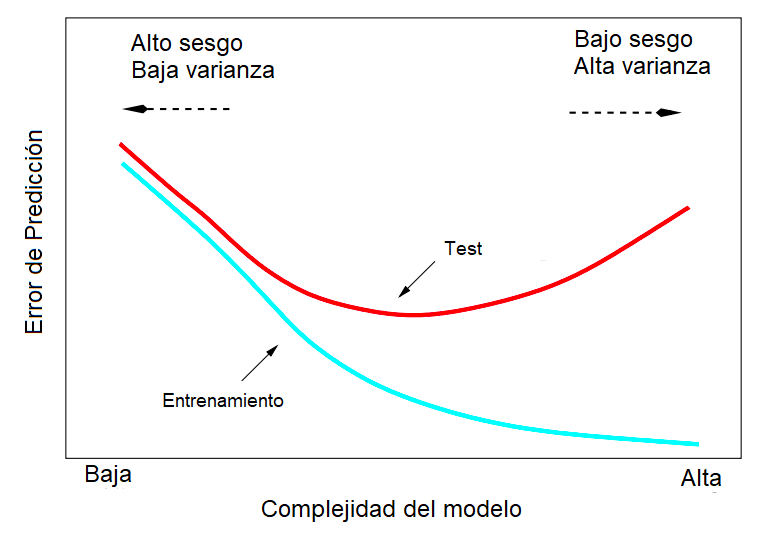
\includegraphics[width=0.7\textwidth]{Kap1/tradeoff.png} 
  \end{center}
 \caption{ Error de test y de entrenamiento en función de la complejidad del modelo. Créditos: \protect\cite{statisticallearning} }
\label{fig:tradeoff}
\end{figure}

\section{Antecedentes relevantes a esta tesina}

\par Como se adelantó anteriormente, en esta tesina se estudiará la aplicación de algoritmos de aprendizaje automatizado al problema de clasificar estrellas variables de tipo RRL en los datasets publicados por Carpyncho, correspondientes al relevamiento VVV. \\

\par Previamente, se ha explorado el desempeño de clasificadores automatizados de estrellas variables en varios estudios \cite{ej1}, \cite{ej2}, \cite{ej3}, \cite{ej4}.  Los dos antecedentes más relevantes de esta tesina, \cite{elorrieta} y \cite{jbc}, proponen procedimientos automatizados para clasificar RRL de subtipo ab en la VVV, basándose en sus curvas de luz. \\

En \cite{elorrieta} se concluye que AdaBoost\cite{adaboost}, un método basado en ensambles de árboles, obtiene consistentemente el mejor desempeño de entre una amplia selección de algoritmos de aprendizaje automatizado incluyendo SVM y redes neuronales profundas. El desempeño es estimado utilizando cross-validation, y a través de la comparación entre dos datasets que fueron clasificados por expertos humanos. Nótese que varias de las métricas utilizadas en este trabajo, como AUC o $F_1$, no son adecuadas para trabajar con datasets altamente desbalanceados. \\

Posteriormente, en \cite{jbc}, se refinaron las métricas de desempeño y se extiende el conjunto de atributos utilizado para describir estrellas variables, incorporando atributos de pseudocolor. En uno de los experimentos, se realizó una comparación entre el desempeño de distintos métodos de clasificación, incluyendo Random Forests y SVM. El mayor desempeño se obtuvo, nuevamente, utilizando ensambles de árboles.


\section{ Comparación entre Random Forest y Support Vector Machines}

Como ya se ha mencionado, Random Forest y SVM son dos potentes métodos de aprendizaje automatizado, que pueden ser aplicados tanto a problemas de regresión como de clasificación. En esta sección, se hará hincapié en ciertas características que distinguen ambos métodos, buscando comparar y contrastar la forma en que ambos operan. El objetivo es enumerar razones que puedan explicar por qué Random Forest parece funcionar mejor que SVM en estudios previos de clasificación de RRL.\\

En primer lugar, se debe notar que ambos métodos proceden de formas radicalmente distintas. En la fase de training, los árboles de decisión que conforman un random forest observan cada feature una a la vez, analizando si es beneficioso realizar divisiones para ciertos valores \cite{mitchell}. Por otro lado, las SVM consideran cada elemento del dataset como un punto en el espacio, utilizando los valores de todas las features en simultáneo para calcular un hiperplano separador \cite{svm2}. \\

Una primera consecuencia es que RF es inmune a \textbf{diferentes escalas} en las features \cite{statisticallearning}. Los datos no necesitan estar normalizados ni centrados para que RF funcione, mientras que la naturaleza geométrica de SVM implica que los distintos atributos necesariamente han de estar expresados en la misma escala \cite{svm_practical}. Más aún, las rutinas de optimización que usualmente implementan la fase de training en SVM pueden fallar en converger, o tardar significativamente más tiempo, si los datos no se encuentran escalados a [0,1] o [-1,1]
\cite{svm_practical}. Por lo tanto, resulta vital realizar un preprocesamiento adecuado a los datos a la hora de aplicar SVM. \\ 

Una segunda consecuencia es que RF puede \textbf{ignorar features que no son muy informativas} fácilmente, pues los árboles de decisión tienen un mecanismo simple para darse cuenta de que no sirven (ningún split será un buen candidato) \cite{statisticallearning}. De acuerdo a \cite{statisticallearning}, los árboles de decisión ``realizan una selección de variables internamente como una parte integral en su forma de proceder''. Ignorar features no informativas puede ser más complejo para SVM, pues la rutina de optimización tendrá que asignar un valor nulo a los coeficientes correspondientes en $w$. Una cierta feature puede ser poco informativa por distintos motivos: puede haber sido incluida en el dataset pero no contener información relevante para predecir la variable target, puede ser extremadamente ruidosa, etc.  Las técnicas de Feature Selection que se aplicarán en capítulos posteriores son una forma adecuada de deshacerse de atributos no informativos, y deberían reducir el impacto de este problema en SVM. \\

Una tercera consecuencia es que RF no se ve afectado por \textbf{features altamente correlacionadas}, pues cada árbol de decisión se dará cuenta fácilmente de que no es informativo realizar el mismo split en dos features correlacionadas \cite{rf_collinearity}. Por otro lado, puede ser más complejo para SVM aprender a ponderar correctamente información redundante. Por tal motivo, es interesante explorar correlaciones entre features y analizar el impacto de eliminar redundancias en los datos. \\

Otro punto a considerar es cómo manejar el \textbf{overfitting} (sobreajuste) durante la fase de training. SVM requiere una cuidadosa estimación del hiperparámetro de regularización C para controlar este fenómeno, mientras que Random Forest por su naturaleza de ensamble es inmune a sobreajustar al aumentar el número de árboles \cite{rf}. Más aún, si se utiliza un kernel con parámetros adicionales como RBF en SVM, se requiere estimar cuidadosamente otros \textbf{hiperparámetros}, por ejemplo realizando Cross Validation Grid Search \cite{svm_practical}. Contrariamente, Random Forest es considerado un método off-the-shelf \cite{offshelf}, pues suele producir buenos resultados sin una optimización de hiperparámetros meticulosa. Por lo tanto, resulta de vital importancia una cuidadosa optimización de hiperparámetros de regularización y de kernel en SVM. \\

El marcado \textbf{imbalance de clases} presente en los datos, con aproximadamente 2000 elementos de clase negativa (no-RRL) por cada elemento de clase positiva (RRL), puede afectar negativamente el desempeño de RF y SVM. En \cite{jbc}, se determinó que corregir el imbalance de clases de estos datos mediante undersampling conduce a una pérdida de desempeño en Random Forest, siendo conveniente entrenar los modelos utilizando los datos sin balancear. Por otro lado, es posible que esto no sea cierto para SVM, dado que el imbalance de clases puede ocasionar pérdida de performance pues el hiperplano soporte elegido estará más alejado de la clase positiva, y habrá mayor cantidad de vectores soporte de la clase negativa \cite{imbalanced_svm}. Resulta por lo tanto interesante explorar diversas técnicas de undersampling y oversampling a la hora de aplicar SVM. \\

La existencia de \textbf{features ruidosas y outliers} en los datos es de esperarse en datasets astronómicos, que pueden incluir errores de medición y observación. RF no se ve afectado por outliers, pues los árboles de decisión funcionan creando cubetas (bins) que no se ven influenciadas por valores extremos \cite{statisticallearning}. Features que son altamente ruidosas no serán informativas a la hora de dividir la clase objetivo, y podrán ser ignoradas por los árboles de decisión. Es interesante explorar distintos preprocesamientos tendientes a limpiar o suavizar los datos a la hora de aplicar SVM, pues puede ayudar a mitigar el efecto de outliers y ruido en los datos. \\

La siguiente tabla resume los puntos discutidos en esta sección. Durante el resto de este trabajo, se explorará cada uno de ellos. 

\begin{table}[h!]
\begin{tabular}{|l|l|}
\hline
\textbf{Aspecto}                                                                            & \textbf{Capítulo Relevante}                                  \\ \hline
\begin{tabular}[c]{@{}l@{}}Estimación de hiperparámetros óptimos\\ Overfitting\end{tabular} & Capítulos 2, 3.                                              \\ \hline
Diferentes escalas en los datos                                                             & Capítulo 4: Preprocesamientos                                \\ \hline
\begin{tabular}[c]{@{}l@{}}Features ruidosas\\ Existencia de outliers\end{tabular}          & Capítulo 4: Preprocesamientos                                \\ \hline
Features no informativas                                                                    & Capítulo 5: Feature selection y \\
 &  feature extraction \\ \hline
Features altamente correlacionadas                                                          & Capitulo 6: Inspeccionando los datos                         \\ \hline
Imbalance de clases                                                                         & Capítulo 7: Imbalance de clases                              \\ \hline
\end{tabular}
\end{table}

Finalmente, en los capítulos 8 y 9 se ponderarán distintas teorías en base a los resultados obtenidos, y se extraerán conclusiones.






 
\chapter{Clasificación de estrellas RRL utilizando Random Forest}

El objetivo de esta sección es determinar la performance de clasificadores Random Forest aplicados a la tarea de clasificar estrellas variables de tipo RRL. Estos resultados serán utilizados como punto de referencia en secciones posteriores, donde se trabajará con clasificadores basados en Support Vector Machines sobre los mismos datos. La implementacion de Random Forest utilizada es la provista por Scikit-Learn \cite{sklearn_api} \cite{pedregosa2011scikit}.

\section{Optimización de hiperparámetros}

Se realizó un experimento utilizando una metodología muy similar a la descripta en la sección ``Model Selection" de \cite{jbc}. En primer lugar, se optimizaron los hiperparámetros de Random Forest utilizando 10-fold Cross Validation Grid Search sobre el tile b278. Los hiperaparámetros a optimizar fueron:

\begin{itemize}
\item \textbf{$n\_estimators$}: El número de árboles en cada ensamble. Se exploró un amplio rango de valores entre 10 y 750 árboles.
\item \textbf{$max\_AUPRCs$}: El número de atributos a considerar cuando se busca el mejor split. Las opciones exploradas fueron la raíz cuadrada del número de atributos (``sqrt"), y el logaritmo en base dos del número de atributos (``log2").
\item \textbf{$criterion$}: La función utilizada para medir la calidad de cada split. Las opciones consideradas fueron Gini Impurity (``gini") e Information Gain (``entropy")
\end{itemize}

La medida de performance utilizada fue el área bajo la curva de precision-recall. Los resultados completos pueden observarse en la figura \ref{fig:optimisationrf}. Las siguientes conclusiones se desprenden de este experimento:

\begin{itemize}
\item Utilizar entropy como criterion es consistentemente más beneficioso que utilizar gini.
\item A partir de aproximadamente 200 árboles, la ganancia de agregar más árboles al ensamble es muy pequeña. A partir de aproximadamente 400 árboles, la ganancia de agregar más árboles parece ser nula.
\item Los hiperparámetros óptimos resultaron ser: $criterion$=``entropy", $n\_estimators$=400 y $max\_features$=``sqrt"
\end{itemize}

\begin{figure}[h!]
\begin{center}
  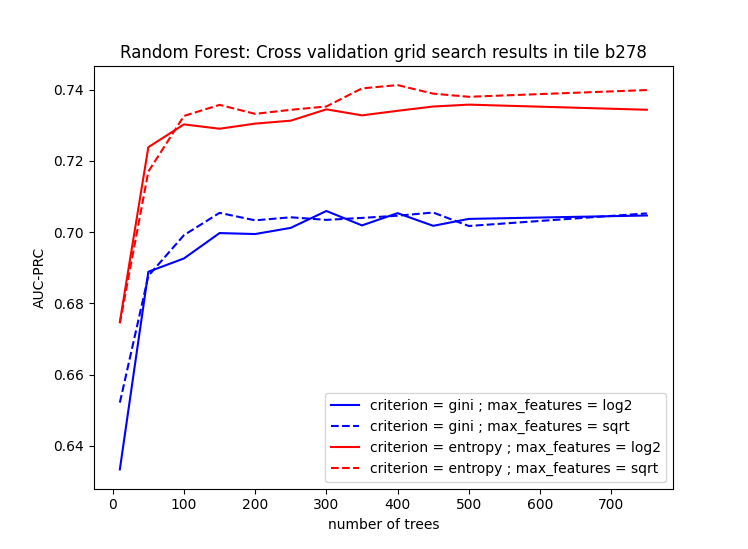
\includegraphics[width=.6\textwidth]{Kap2/Figure_1.png}
  \end{center}
  \caption{Resultados de la optimización de hiperparámetros de Random Forest en el tile b278}
  \label{fig:optimisationrf}
\end{figure}

\section{ Análisis de performance de Random Forest }

Para estimar la performance de Random Forest utilizando los parámetros óptimos que se obtuvieron en la sección anterior, se utilizará un subconjunto fijo de tiles: \{ b234, b261 , b278, b360 \}. Este subconjunto de tiles fue escogido como un compromiso entre la densidad y cobertura de estrellas de tipo RRL\cite{jbc}. Para cada par de tiles $t_1$ y $t_2$, se entrenará un clasificador Random Forest utilizando $t_1$ como dataset de training y $t_2$ como dataset de test, obteniendo curvas de precision-recall. \\

Las curvas resultantes pueden observarse en la figura \ref{fig:testresults}, en color azul. Los valores obtenidos son consistentes con aquellos reportados en trabajos previos \cite{jbc}. Pueden observarse diversos comportamientos, dependiendo de los datos de training y testing seleccionados. En la mayoría de los casos, parece ser posible fijar un recall de 0.5 y obtener una precisión igual o mayor a 0.5. Si se desea una mayor precisión, por ejemplo 0.9; parece ser posible fijar un recall de 0.2 para obtenerla. Esto significa que, utilizando random forests, sería posible detectar automáticamente y con alta precisión al menos el 20\% de las RLL mapeadas por el VVV.



\begin{comment}


\begin{figure}[h]
\begin{center}

\begin{tabular}{ccc}

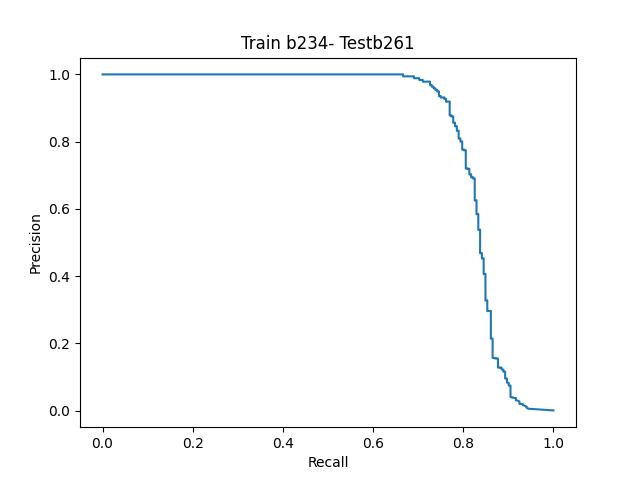
\includegraphics[width=0.32\textwidth]{"Kap2/rf_test_results_train=b234Test=b261.png"} &
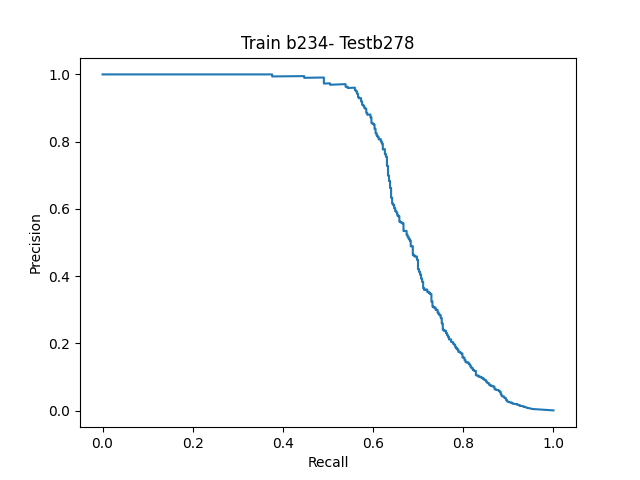
\includegraphics[width=0.32\textwidth]{"Kap2/rf_test_results_train=b234Test=b278.png"} &
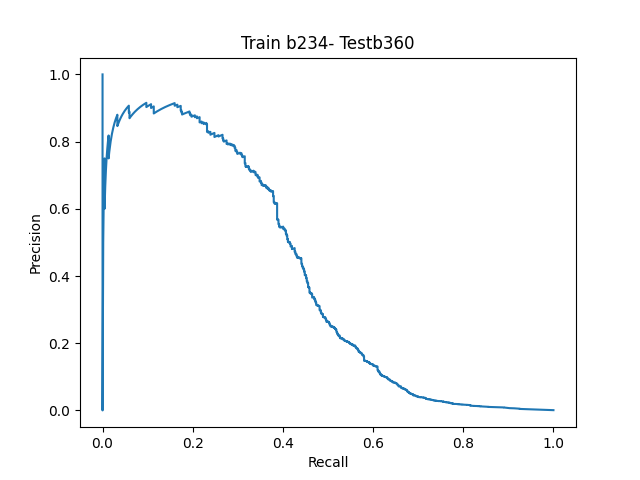
\includegraphics[width=0.32\textwidth]{"Kap2/rf_test_results_train=b234Test=b360.png"} \\

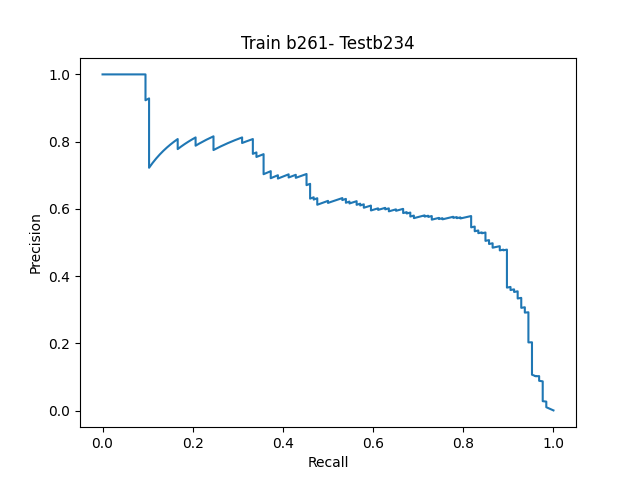
\includegraphics[width=0.32\textwidth]{"Kap2/rf_test_results_train=b261Test=b234.png"} &
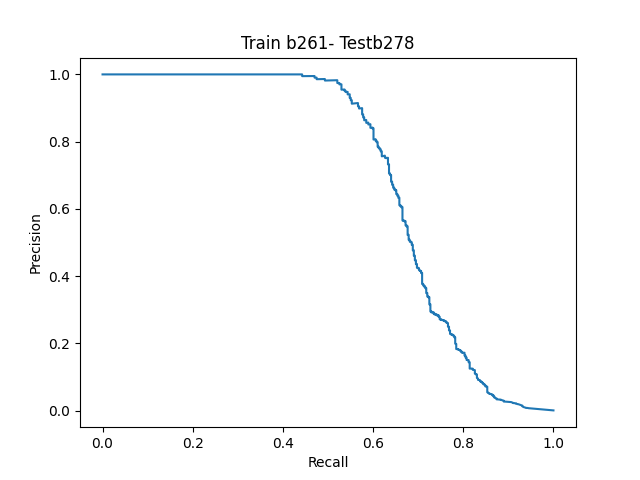
\includegraphics[width=0.32\textwidth]{"Kap2/rf_test_results_train=b261Test=b278.png"} &
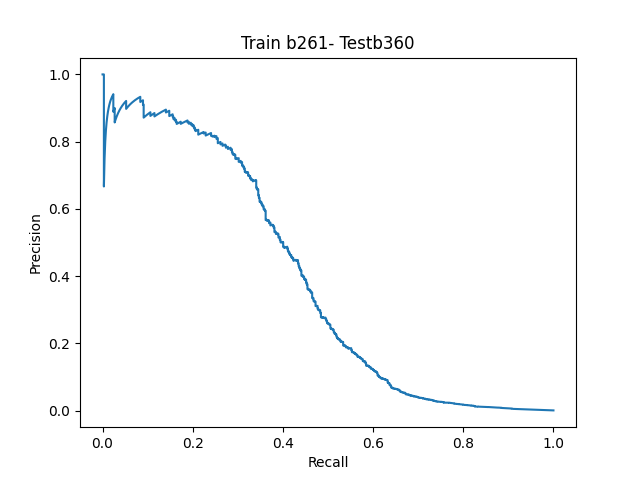
\includegraphics[width=0.32\textwidth]{"Kap2/rf_test_results_train=b261Test=b360.png"} \\

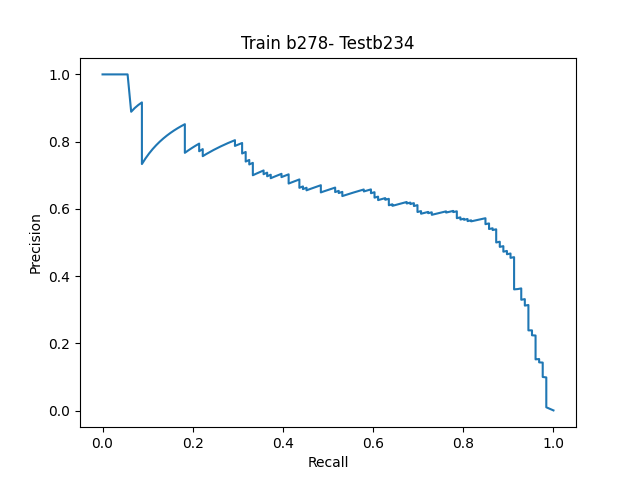
\includegraphics[width=0.32\textwidth]{"Kap2/rf_test_results_train=b278Test=b234.png"} &
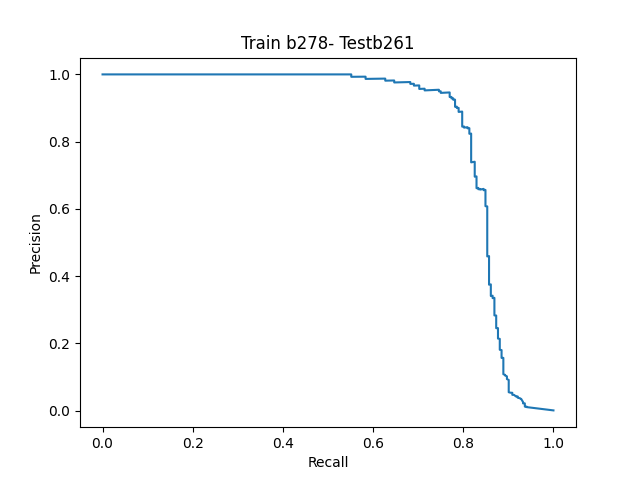
\includegraphics[width=0.32\textwidth]{"Kap2/rf_test_results_train=b278Test=b261.png"} &
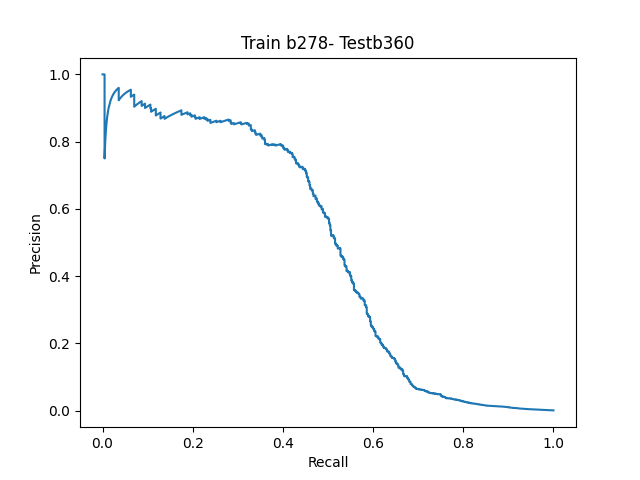
\includegraphics[width=0.32\textwidth]{"Kap2/rf_test_results_train=b278Test=b360.png"} \\

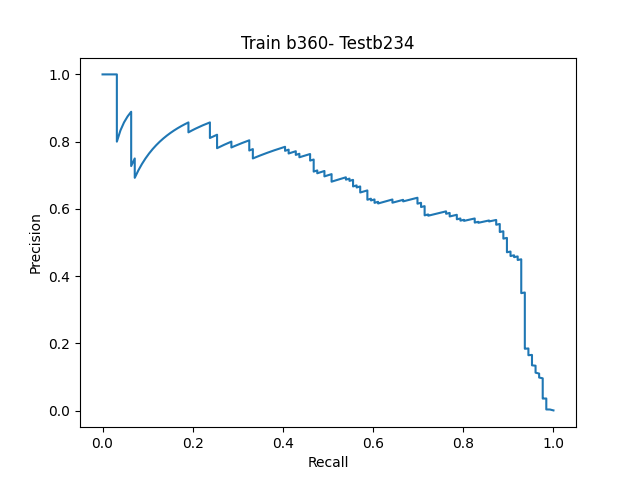
\includegraphics[width=0.32\textwidth]{"Kap2/rf_test_results_train=b360Test=b234.png"} &
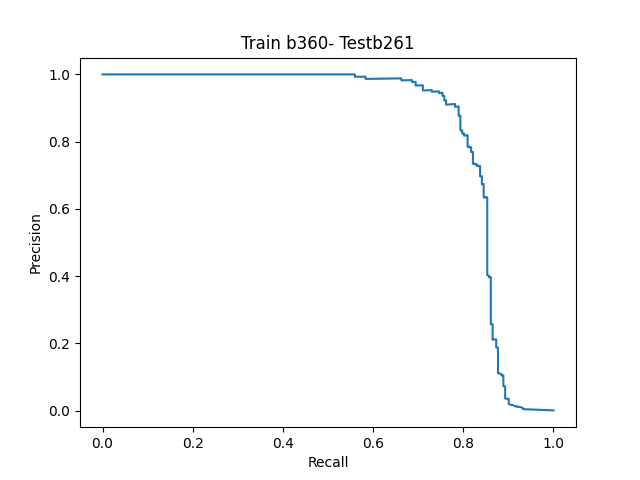
\includegraphics[width=0.32\textwidth]{"Kap2/rf_test_results_train=b360Test=b261.png"} &
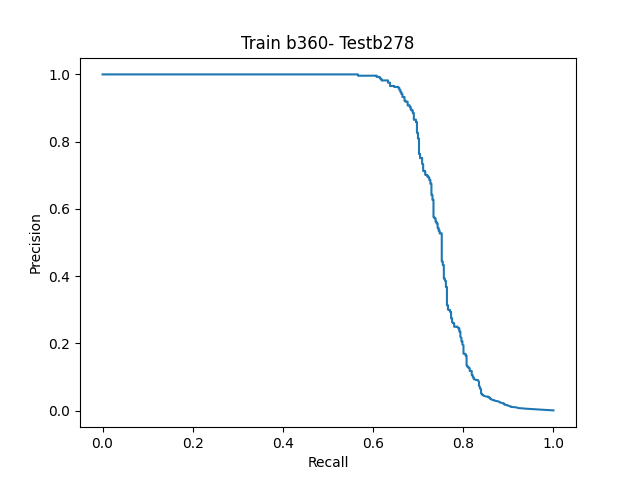
\includegraphics[width=0.32\textwidth]{"Kap2/rf_test_results_train=b360Test=b278.png"}

\end{tabular}

\end{center}
\caption[short]{Curvas de precision-recall obtenidas utilizando Random Forest}
\label{fig:testresultsrf}
\end{figure}


\end{comment}


\chapter{Clasificación de estrellas RRL utilizando Support Vector Machines}

En este capítulo se repitieron los experimentos descriptos en el capítulo anterior, utilizando SVM en vez de RF. Esto permitirá realizar una primera comparación entre el desempeño de ambos métodos. \\

En trabajos previos se ha reportado que la performance de SVM es inferior a la de métodos basados en ensembles de árboles a la hora de clasificar estrellas variables de tipo RRL \cite{jbc} \cite{elorrieta}. El objetivo de este capítulo es reproducir estos resultados, obteniendo un baseline de performance para SVM que intentaremos mejorar y entender en capítulos posteriores. \\

Nuevamente se utilizaron implementaciones de SVM provistas por SciKit Learn\cite{sklearn_api} \cite{pedregosa2011scikit}. Para todos los experimentos de esta sección, se aplicó un escalado estándar a los tiles de training y testing antes de utilizarla (restando la media en training de cada feature y dividiendo por la varianza en training).

\section{Optimización de hiperparámetros para SVM Lineal}

En primera instancia, se utilizó SVM con kernel lineal. Se utilizó la implementacion \textbf{LinearSVC} de SciKit Learn, la cuál está implementada en terminos de liblinear \cite{liblinear}. Esta implementación se caracteriza por escalar casi linealmente a datasets con millones de elementos, lo cual nos permite entrenar con tiles completas. \\

Para optimizar el parámetro de regularización C, se realizó 10-fold Cross Validation Grid Search sobre el tile b278. Se exploró un amplio rango de valores para C, utilizando una escala logarítmica. La medida de performance elegida fue, nuevamente, el area bajo la curva de precision-recall. Adicionalmente se estudió la precisión a valores fijos de recall. En la figura \ref{fig:optimisationsvml} pueden apreciarse los resultados completos de este experimento. \\ 

El valor óptimo encontrado fue C=0.1. Valores pequeños de C conducen a modelos muy pobres, lo cuál indica que modelos donde el margen elegido por SVM es muy grande (permitiendo demasiadas clasificaciones incorrectas) no generan buenos resultados. Por otro lado, incrementar el valor de C más allá de 0.1 tampoco produce mejoras en performance, generando modelos que son innecesariamente más complejos.


\begin{figure}[h!]
\begin{center}
  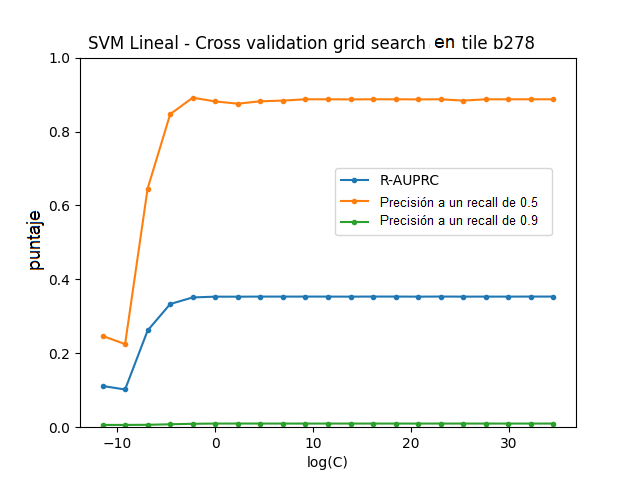
\includegraphics[width=.6\textwidth]{Kap3/Figure_1.png}
  \end{center}
  \caption{Resultados de la optimización de hiperparámetros de SVM-Lineal en el tile b278}
  \label{fig:optimisationsvml}
\end{figure}


\section{Aproximando SVM Kernel}
En la sección \ref{trick} se introdujo el truco del kernel, que consiste en mapear puntos desde un espacio de menor dimensionalidad a un espacio de mayor dimensionalidad. Un punto clave es que, en realidad, únicamente se computan los productos internos en el espacio de mayor dimensionalidad, y nunca es necesario mapear los datos realmente a este espacio. \\

Sin embargo, una de las características de los algoritmos que utilizan este tipo de truco, como SVM kernel, es que su complejidad temporal escala con el número de instancias de entrenamiento ($\mathcal{O}(n^3)$), en tanto que la complejidad espacial será cercana a $\mathcal{O}(n^2)$. Esto implica que se vuelve prohibitivo utilizar SVM kernel en los tiles de Carpyncho, que tienen cientos de miles de instancias cada uno. \\

En resumidas cuentas, SVM kernel funciona muy bien en datos que no son linealmente separables, pero no escala bien a datasets con muchas instancias. Por otro lado, como se mencionó en la sección anterior, existen implementaciones de SVM Lineal que escalan de forma lineal a la cantidad de instancias de entrenamiento. \\

Una tendencia reciente es combinar ambos, dejando de lado la idea fundamental del truco del kernel. La idea base es mapear los datos literalmente a un espacio de mayor dimensionalidad y luego aplicar un clasificador lineal, el cuál generará fronteras de decisión no lineales en el espacio original. \\

Dado que algunos kernels, como RBF, mapean los datos a un espacio de infinitas dimensiones; se busca mapear los datos a un espacio con una cantidad finita razonablemente grande de dimensiones. Afortunadamente, se sabe que únicamente un subespacio finito de este espacio con infinitas dimensiones es necesario para resolver el problema de SVM: el espacio inducido por las imágenes de los datos de entrenamiento. \\

Sin embargo, mapear a este espacio inducido sería al menos tan costoso como SVM kernel exacto. Una solución aproximada es utilizar solo un subconjunto de $m<n$ puntos de entrenamiento para generar un mapeo a $\mathbb{R}^m$. Este algoritmo es llamado Método de Nystroem, y permite obtener un mapeo aproximado, pudiéndose controlar la complejidad asociada ajustando el parámetro $m$. \\

Los detalles del procedimiento recien descripto pueden consultarse en las siguientes publicaciones: \cite{nystroem}, \cite{NIPS2012_621bf66d}, \cite{NIPS2007_013a006f}.

\section{Optimización de hiperparámetros para SVM RBF}

En este segundo experimento, se utilizó SVM con un kernel no lineal: Radial Basis Function. La optimización de hiperparámetros se vuelve significativamente más costosa, dado que se deben optimizar los parámetros $C$ y $\gamma$ en simultáneo. Adicionalmente, debido al inmenso tamaño de nuestros tiles (aproximadamente 400000 filas cada uno), resultó computacionalmente prohibitivo utilizar implementaciones puras de kernel SVM, cuya complejidad es $\mathcal{O}(n_{atributos} \times n_{instancias}^2)$ \cite{libsvm}. \\

Se decidió utilizar un aproximador del kernel RBF, Nystroem, seguido de la eficiente implementación de LinearSVC descripta en la sección anterior. Esto permite aproximar los resultados de kernel SVM, reduciendo dramáticamente la complejidad computacional requerida.\\

Durante el experimento, se realizó 10-fold Grid Search Cross Validation sobre el tile b278. Se exploró un amplio rango logarítmico de valores para los hiperparámetros $\alpha$ y $C$. Los resultados pueden observarse en \ref{fig:optimisationsvmk}. 

\begin{figure}[h!]
\begin{tabular}{cc}
  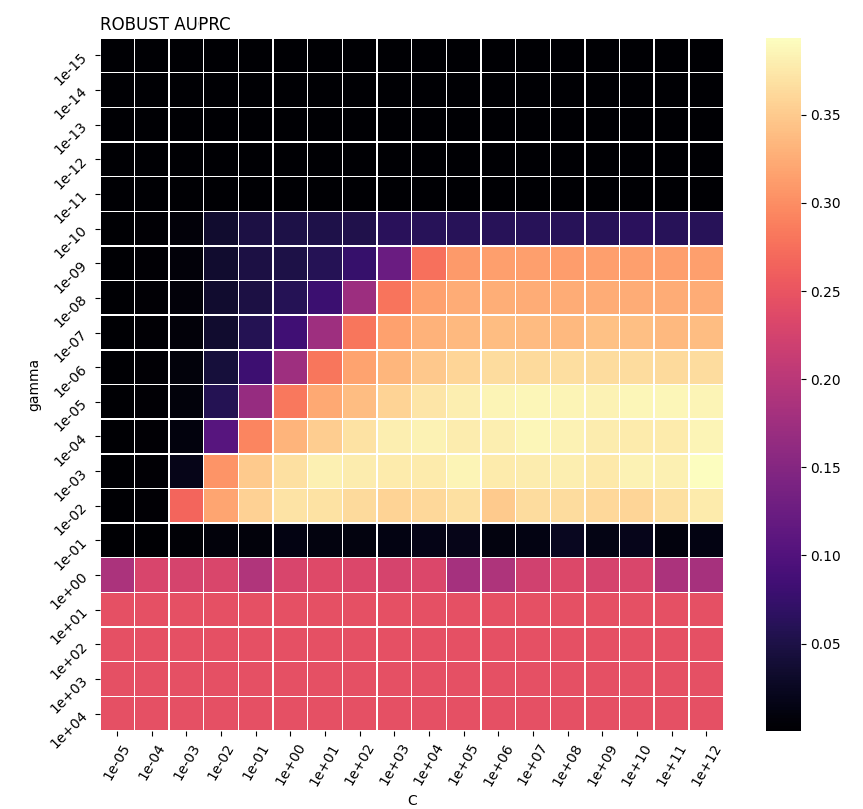
\includegraphics[width=0.49\textwidth]{Kap3/Figure_2.png} &   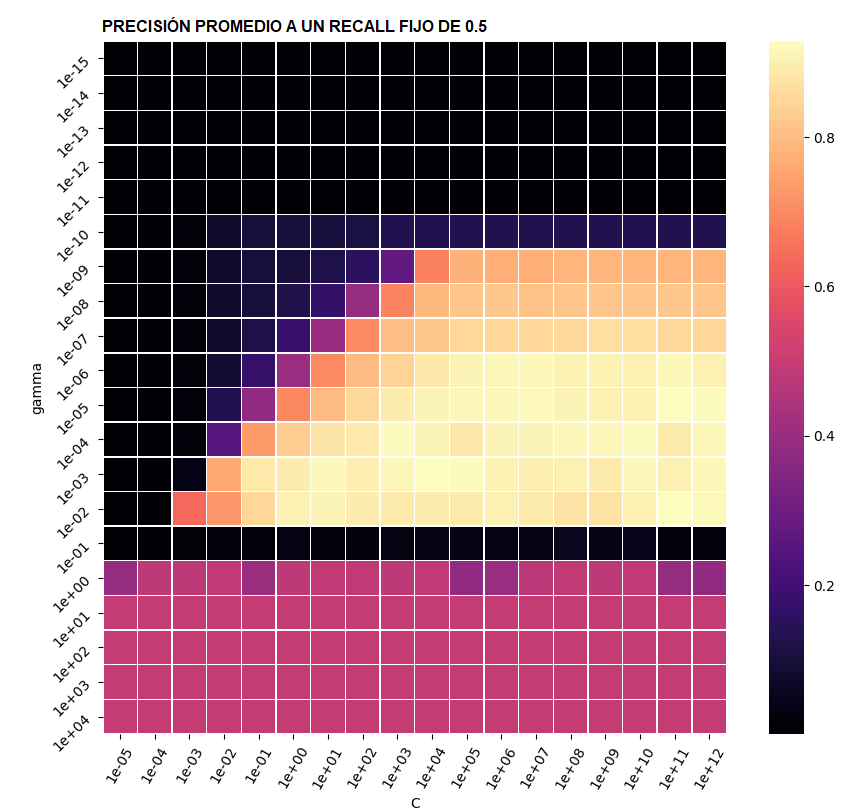
\includegraphics[width=0.49\textwidth]{Kap3/Figure_3.png} \\
(a) Area bajo la curva de Precision-Recall & (b) Precision a un recall fijo de 0.5 
\end{tabular}
\caption{Resultados de la optimización de hiperparámetros para SVM-RBF en el tile b278}
\label{fig:optimisationsvmk}
\end{figure}


Podemos observar que SVM-RBF es muy sensible a la elección de hiperparámetros, a diferencia de RF que no se ven muy afectados por la elección del número de árboles. Los hiperparámetros óptimos fueron $C=10^5$ y $\gamma=10^{-4}$.

\section {Análisis de performance de SVM}

Habiendo estimado los hiperparámetros óptimos de SVM con kernel lineal y RBF, se procedió a entrenar y testear clasificadores usando cada par de tiles en \{ b234, b261 , b278, b360 \}. Las curvas de precision-recall de ambos modelos, así como las de random forest, pueden observarse en la figura \ref{fig:testresults}. \\

\begin{figure}[h!]
\begin{center}

\begin{tabular}{ccc}
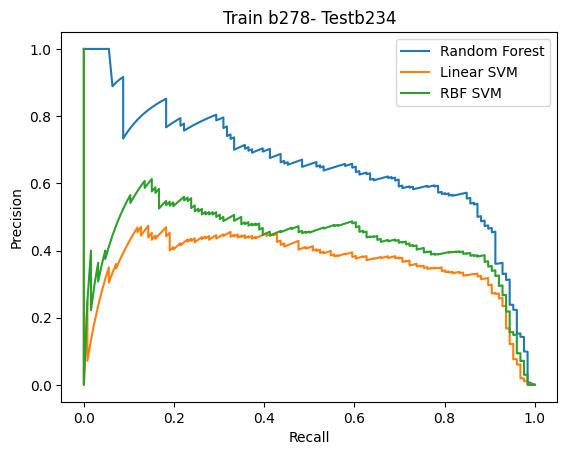
\includegraphics[width=0.32\textwidth]{Kap3/test_results_train=b278Test=b234.png} &
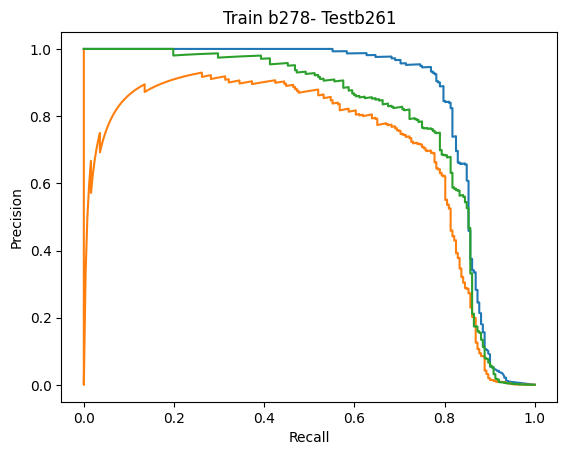
\includegraphics[width=0.32\textwidth]{Kap3/test_results_train=b278Test=b261.png} &
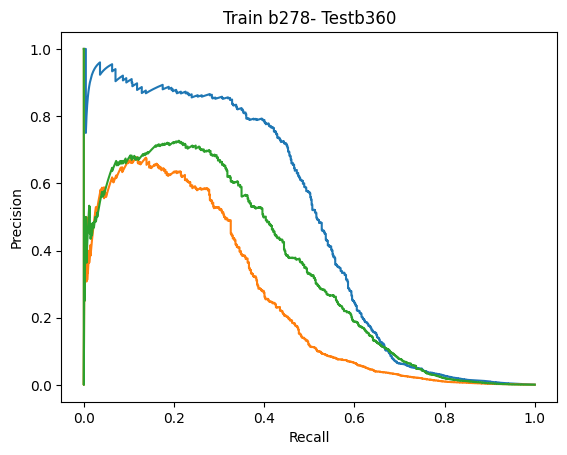
\includegraphics[width=0.32\textwidth]{Kap3/test_results_train=b278Test=b360.png} \\

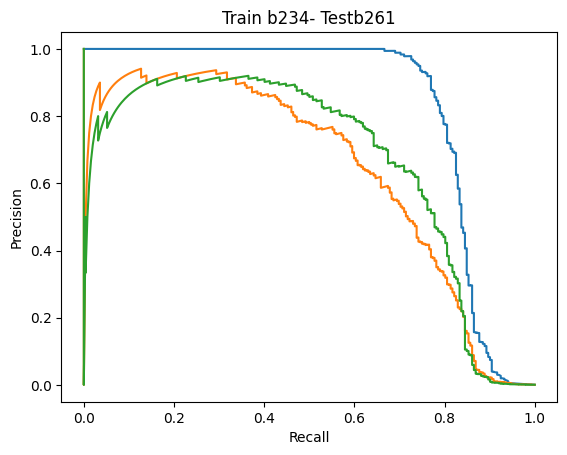
\includegraphics[width=0.32\textwidth]{Kap3/test_results_train=b234Test=b261.png} &
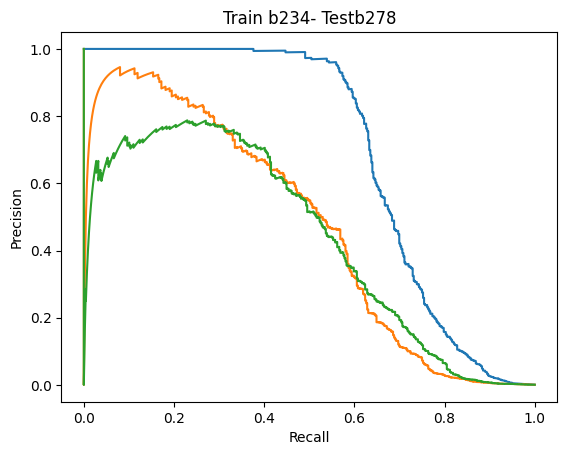
\includegraphics[width=0.32\textwidth]{Kap3/test_results_train=b234Test=b278.png} &
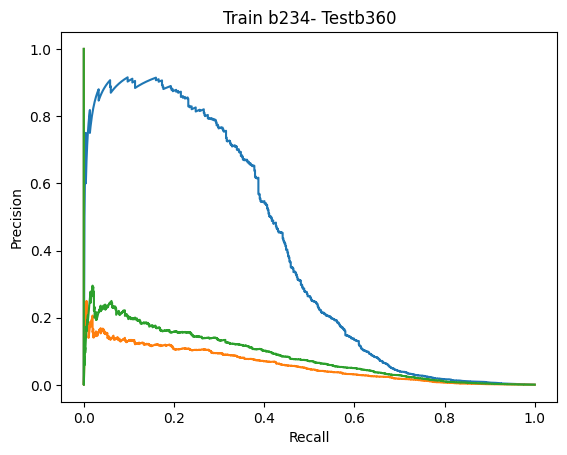
\includegraphics[width=0.32\textwidth]{Kap3/test_results_train=b234Test=b360.png} \\

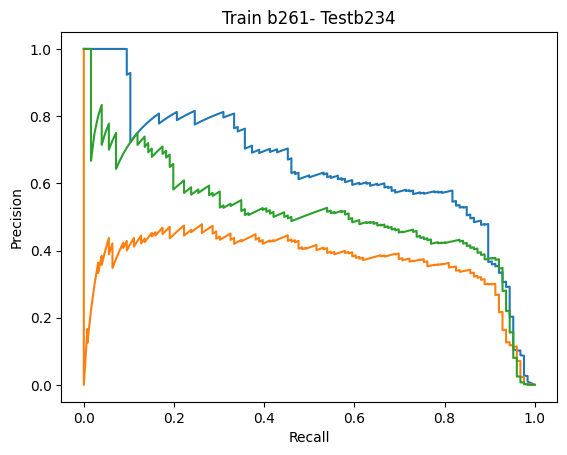
\includegraphics[width=0.32\textwidth]{Kap3/test_results_train=b261Test=b234.png} &
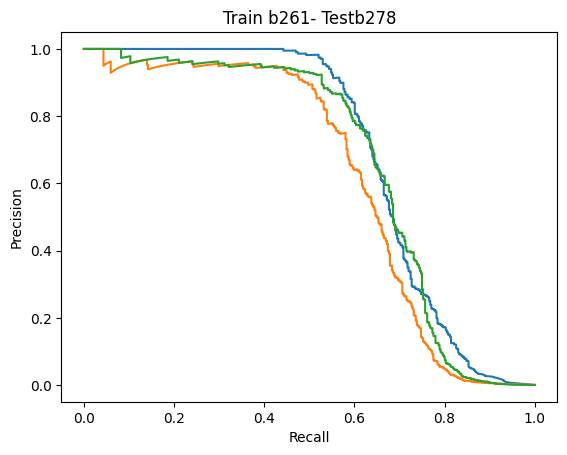
\includegraphics[width=0.32\textwidth]{Kap3/test_results_train=b261Test=b278.png} &
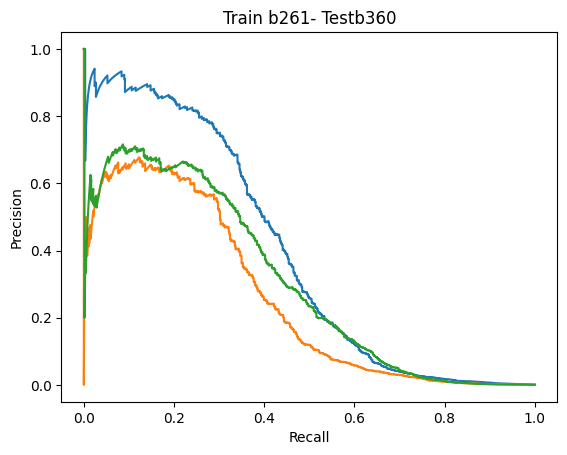
\includegraphics[width=0.32\textwidth]{Kap3/test_results_train=b261Test=b360.png} \\

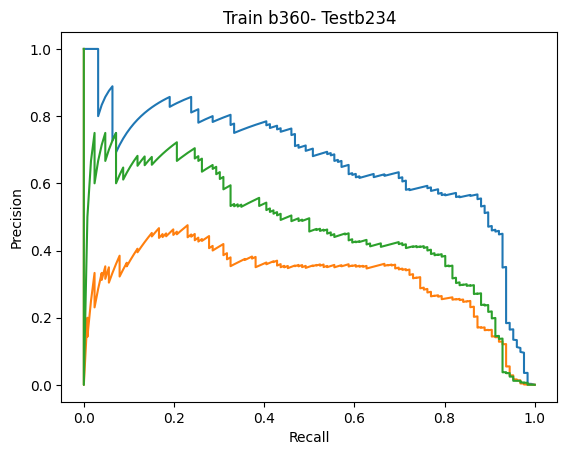
\includegraphics[width=0.32\textwidth]{Kap3/test_results_train=b360Test=b234.png} &
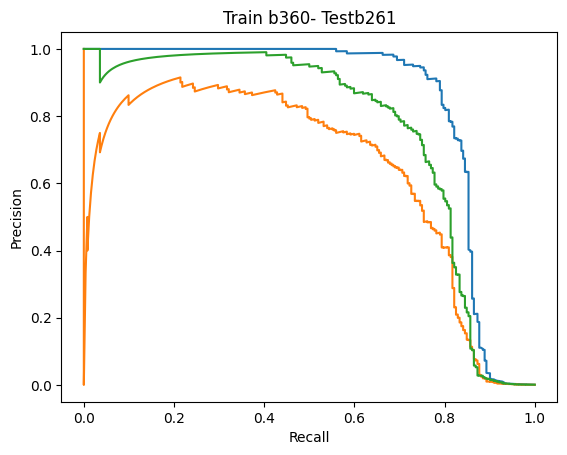
\includegraphics[width=0.32\textwidth]{Kap3/test_results_train=b360Test=b261.png} &
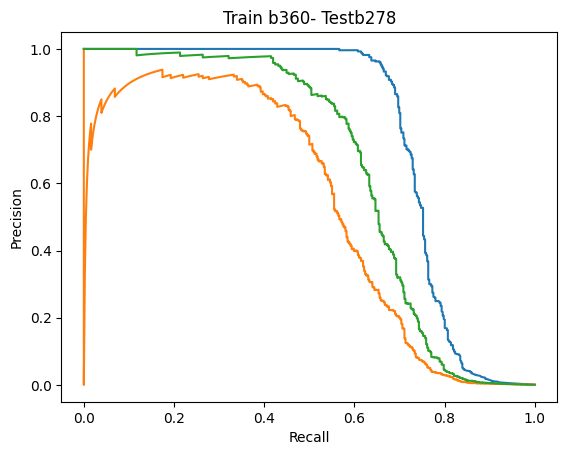
\includegraphics[width=0.32\textwidth]{Kap3/test_results_train=b360Test=b278.png}

\end{tabular}

\end{center}
\caption[short]{Curvas de precision-recall obtenidas utilizando Random Forest, Support Vector Machine con kernel lineal y Support Vector Machine con kernel RBF}
\label{fig:testresults}

\end{figure}

\newpage
Algunas observaciones:

\begin{itemize}

\item En las 12 combinaciones testeadas la performance de random forest es superior a la de SVM-RBF, la cuál es a su vez superior a SVM Lineal. Esto se condice con los resultados reportados en \cite{jbc}. El hecho de haber utilizado las tiles completas para entrenar y testear nos permite apreciar con exactitud cuán mejores son las curvas generadas por Random Forest, lo cuál no era evidente en trabajos previos.

\item El hecho de que SVM Lineal tenga la menor performance parece indicar que la superficie de decisión no es lineal.
\item El hecho de que las curvas varíen tanto para cada par de tiles elegido, indica que los clasificadores se ven altamente influenciados por el tile de train y el tile de test elegido. Esto no sucedería si los samples de todos los tiles estuviesen regidos por la misma distribución de probabilidad subyacente. Dado que cada tile tiene cientos de miles de samples, esto indicaría que los datos de cada tile son inherentemente distintos, de otro modo las curvas de cada clasificador deberían ser muy parecidas entre distintos tiles.
\end{itemize}

En los capítulos siguientes se aplicarán distintas técnicas con el objeto de mejorar las curvas obtenidas por SVM. Adicionalmente, se intentará comprender por qué RF parece funcionar mucho mejor que SVM en este tipo de datos.
\chapter{Preprocesamientos}

En este capítulo se describirán distintos tipos de preprocesamientos que pueden ser aplicados a los datos. Posteriormente, se procederá a realizar experimentos utilizando cada uno de estos preprocesamientos en combinación con SVM, evaluando si hay alguna mejora en los resultados que fueron expuestos en el capítulo anterior. Se utilizarán las implementaciones provistas por el módulo \textit{preprocessing} de SKLearn \cite{sklearn_api}, cuyos detalles pueden consultarse en la documentación de SKLearn\footnote{ \url{https://scikit-learn.org/stable/modules/preprocessing.html} }. 

\section { Estandarización }

En primer lugar, se consideraron distintas técnicas básicas que consisten en modificar la media y escalar la varianza de los datos. \cite{han2012mining}

\begin{itemize}
\item \textbf{MaxAbsScaler}: Escalar cada atributo por separado al rango $[-1,1]$. Para cada columna $c$, se dividen todos los elementos de esa columna por su máximo valor absoluto:

\begin{center}
$ c := \frac{c}{max(abs(c))} $
\end{center}

\item \textbf{MinMaxScaler}: Escalar cada atributo por separado al rango $[0,1]$. Para cada columna $c$, se aplica la siguiente transformación \cite{han2012mining}:

\begin{center}
$ c := \frac{ c - min(c) } { max(c) - min(c) }$
\end{center}

\item \textbf{StandardScaler}: Estandarizar cada atributo, restándole su media y escalando a varianza unitaria.

\begin{center}
$ c := \frac{ c - mean(c) } { stdev(c) }$
\end{center}

\item \textbf{RobustScaler}: Estandarizar cada atributo usando métricas robustas a outliers, restando la mediana y escalando los datos de acuerdo al rango intercuartil.

\end{itemize}

\section { Transformaciones no lineales y discretización}

En esta sección se enumeran distintas técnicas que modifican la distribución de probabilidad subyacente de cada atributo:

\begin{itemize}

\item \textbf{PowerTransformer}: Aplica una transformación paramétrica, monotónica que transforma cada atributo para que tenga una distribución de probabilidad más Gaussiana. La transformación utilizada es  Yeo-Johnson \cite{yeo}. Un escalado estándar (StandardScaler) es aplicado previamente a los datos.

\item \textbf {QuantileTransformer}: Transformar cada atributo por separado, obteniendo valores entre 0 y 1. Una primera opción es mapear los datos a una distribución uniforme, una segunda opción es mapear los datos a una distribución normal \cite{KRZYSZTOFOWICZ1997286}. Un parámetro de esta transformación es el número de cuantiles computado para realizar la transformación.

\item \textbf {Binning}: Discretizar cada atributo por separado, distribuyendo sus valores en $k$ cubetas (bins) \cite{han2012mining}. Distintos criterios pueden seguirse para decidir cómo se distribuyen los datos en cada cubeta:
\begin{itemize}
\item \textbf{Uniforme}: Usar cubetas de tamaño constante. Es decir, dividir el rango de valores del atributo en $k$ intervalos del mismo tamaño; y reemplazar cada valor por el índice de su intervalo.
\item \textbf{Quantile}: Colocar la misma cantidad de elementos en cada cubeta.
\item \textbf{Kmeans}: Definir cada cubeta basado en un algoritmo de clústering k-means. 
\end{itemize}
\end{itemize}


Es importante remarcar que para todos los preprocesamientos discutidos hasta el momento, se estimarán los parámetros de la transformación usando únicamente los datos de entrenamiento. Por ejemplo, los límites de los bins son calculados sobre los datos de entrenamiento y estos mismos límites se utilizarán para discretizar los datos de test. Análogamente, a la hora de realizar un escalado estándar por ejemplo, tanto a los datos de entrenamiento como a los de test se les resta la media del dataset de entrenamiento y se les divide por la varianza del detaset de entrenamiento.

\section { Preprocesamientos en SVM Lineal }

Se aplicaron los preprocesamientos descriptos en las secciones anteriores a los datos, antes de utilizar SVM Lineal. En los siguientes experimentos, se considera como base de referencia la performance reportada en la última sección del capítulo anterior, obtenida aplicando únicamente StandardScaler antes de entrenar y testear. 

\begin{itemize}

\item Los resultados de aplicar estandarización pueden ser observados en \ref{fig:svml_estandarizacion}. De este experimento se desprende que StandardScaler es la mejor opción, dado que es la única opción que se encuentra consistentemente entre los preprocesamientos con mejor performance.

\item Los resultados de aplicar QuantileTransformer se pueden observar en \ref{fig:svml_quantiles}. Se exploraron ambas variantes: mapear la distribución de cada atributo a una distribución normal, y a una distribución uniforme. Para cada una de estas configuraciones, se analizó el R-AUPRC en función del número de cuantiles utilizado en el transformador. Podemos observar que todas las combinaciones de parámetros exploradas efectivamente incrementan la performance respecto a la base de referencia; aunque el número de cuantiles óptimo es dependiente de los datos.

\item Los resultados de aplicar binning, seguido de un escalado estándar, se pueden observar en \ref{fig:svml_binning}. Se exploraron las tres estrategias anteriormente mencionadas (Uniform, Quantile y Kmeans), estudiando la evolución del R-AUPRC en función del número de cubetas. Se puede apreciar que la estrategia Quantile es consistentemente la mejor opción. Nótese que la estrategia KMeans es computacionalmente impracticable para grandes cantidades de cubetas.

\item Las curvas de precision-recall de los preprocesamientos que tuvieron mejor desempeño en los experimentos anteriores, junto con la correspondiente a PowerTransformer (que no requiere parámetros), son comparadas en la figura \ref{fig:svml_final_comparison}. De esta comparación final se desprende que el preprocesamiento óptimo para SVM Lineal es binning, seguido de un escalado estándar. Al final de este capítulo se especula sobre los motivos por los cuales binning produce tales mejoras.
\end{itemize}


\begin{figure}[h!]
\begin{tabular}{cccc}
  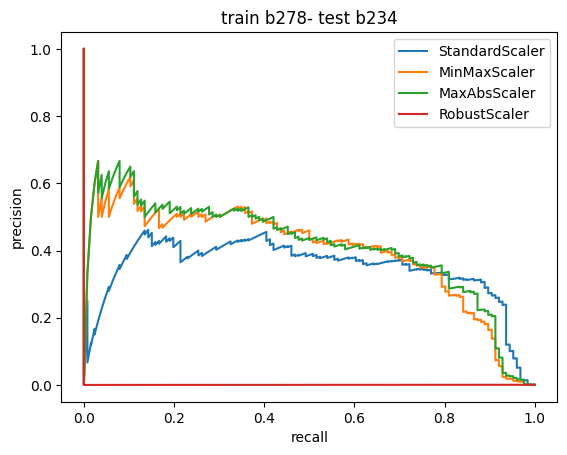
\includegraphics[width=0.25\textwidth]{Kap4/Figure_1.png}  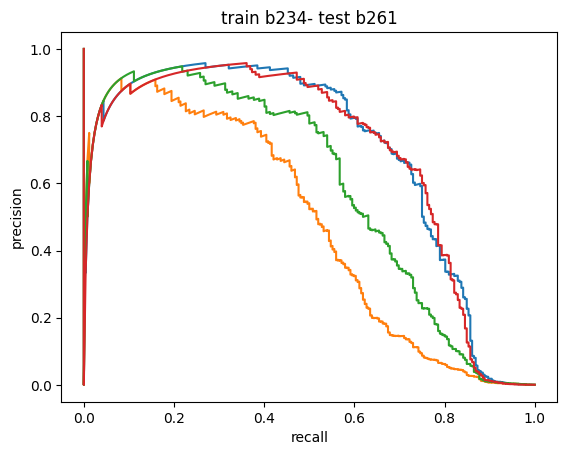
\includegraphics[width=0.25\textwidth]{Kap4/Figure_2.png} 
  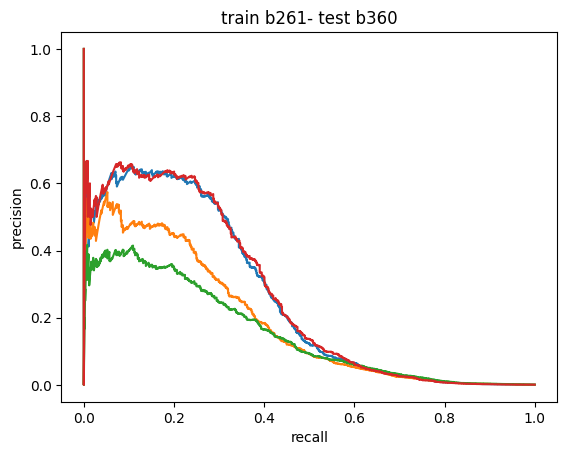
\includegraphics[width=0.25\textwidth]{Kap4/Figure_3.png}  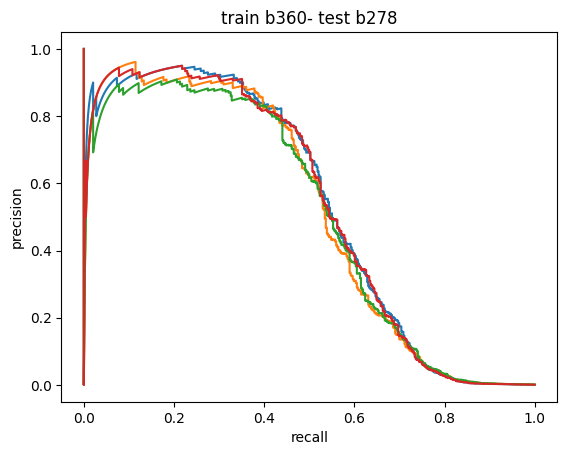
\includegraphics[width=0.25\textwidth]{Kap4/Figure_4.png} 
\end{tabular}
\caption{Estandarización en SVM Lineal.}
\label{fig:svml_estandarizacion}
\end{figure}

\begin{figure}[h!]
\begin{tabular}{cccc}
  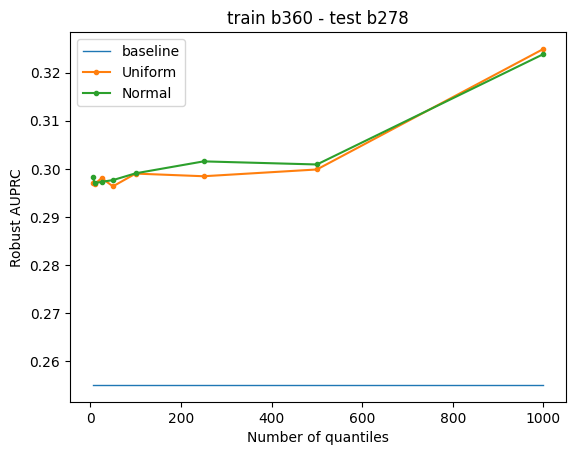
\includegraphics[width=0.25\textwidth]{Kap4/Figure_5.png}  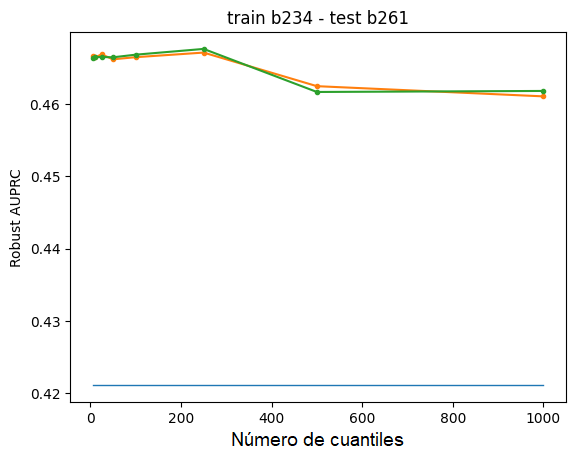
\includegraphics[width=0.25\textwidth]{Kap4/Figure_6.png}
  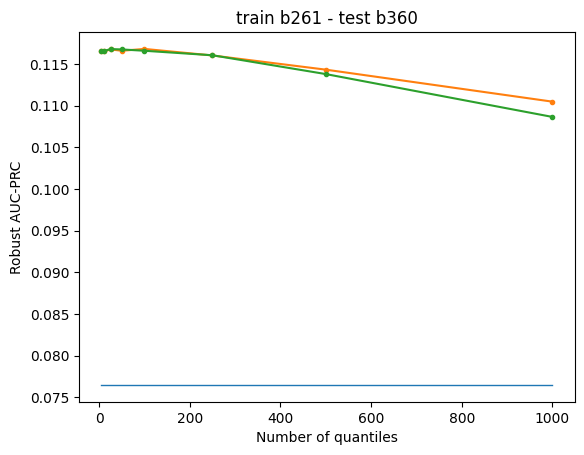
\includegraphics[width=0.25\textwidth]{Kap4/Figure_7.png}  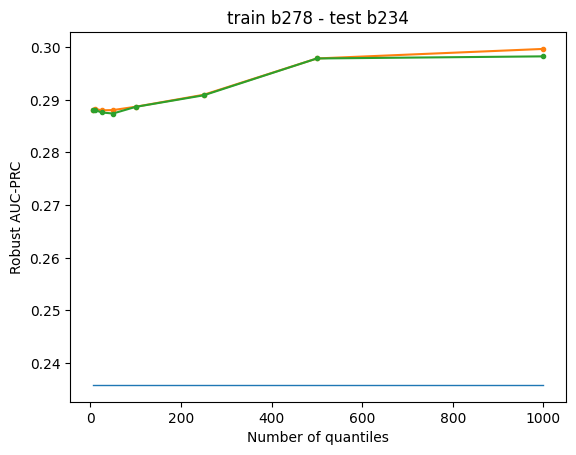
\includegraphics[width=0.25\textwidth]{Kap4/Figure_8.png} 
\end{tabular}
\caption{QuantileTransformer en SVM Lineal}
\label{fig:svml_quantiles}
\end{figure}

\begin{figure}[h!]
\begin{tabular}{cccc}
  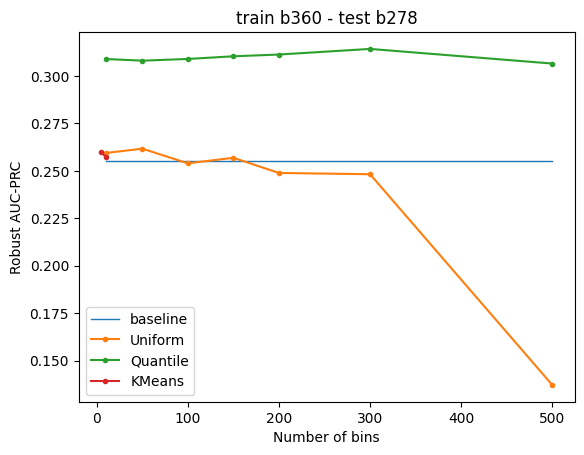
\includegraphics[width=0.25\textwidth]{Kap4/Figure_9.png}  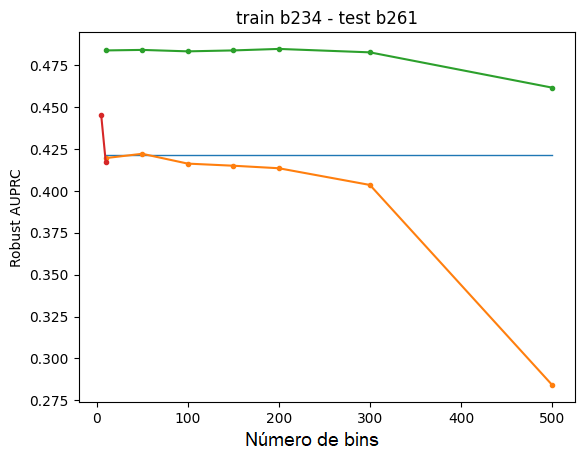
\includegraphics[width=0.25\textwidth]{Kap4/Figure_10.png}
  \includegraphics[width=0.25\textwidth]{Kap4/Figure_11.png} \includegraphics[width=0.25\textwidth]{Kap4/Figure_12.png} 
\end{tabular}
\caption{Binning en SVM Lineal}
\label{fig:svml_binning}
\end{figure}

\begin{figure}[h!]
\begin{tabular}{cccc}
  \includegraphics[width=0.25\textwidth]{Kap4/Figure_13.png}  \includegraphics[width=0.25\textwidth]{Kap4/Figure_14.png}
  \includegraphics[width=0.25\textwidth]{Kap4/Figure_15.png}  \includegraphics[width=0.25\textwidth]{Kap4/Figure_16.png} \\

\includegraphics[width=0.25\textwidth]{Kap4/Figure_17.png}  \includegraphics[width=0.25\textwidth]{Kap4/Figure_18.png} 
 \includegraphics[width=0.25\textwidth]{Kap4/Figure_19.png}  \includegraphics[width=0.25\textwidth]{Kap4/Figure_20.png} 
\end{tabular}
\caption{Comparación de los mejores preprocesamientos, SVM Lineal}
\label{fig:svml_final_comparison}
\end{figure}



\section{Preprocesamientos en SVM RBF}

Se procedió a realizar los mismos experimentos utilizando SVM con kernel RBF:

\begin{itemize}
\item Los resultados de aplicar estandarización pueden ser observados en \ref{fig:svmk_estandarizacion}. Nuevamente, StandardScaler parece ser la mejor opción, estando consistentemente entre los que mejor funcionan. El escalado robusto, si bien produce mejores resultados en ciertos tiles, ocasiona una pérdida significativa de performance en otros.

\item Los resultados de aplicar QuantileTransformer se pueden observar en \ref{fig:svmk_quantiles}. A diferencia de en SVM-Lineal, la performance oscila considerablemente dependiendo del número de cuantiles, y es difícil encontrar una asignación de parámetros para este método que sea óptima para todos los tiles. Más aún, aplicar este preprocesamiento implica una pérdida de performance respecto a la base de referencia en algunas de las combinaciones testeadas, por lo cuál se descarta su aplicación en el resto de este trabajo.

\item Los resultados de aplicar binning, seguido de un escalado estándar, se pueden observar en \ref{fig:svmk_binning}. Los resultados son consistentes a los observados en SVM Lineal: La estrategia Quantile es consistentemente superior a las otras estrategias, y dependiendo del número de bins escogido mejora la performance respecto a la base de referencia. 

\item Las curvas de precision-recall de los preprocesamientos que tuvieron mejor desempeño en los experimentos anteriores, junto con la correspondiente a PowerTransformer (que no requiere parámetros), son comparadas en la figura \ref{fig:svmk_final_comparison}. De esta comparación final se desprende que el preprocesamiento óptimo para SVM RBF es Binning, aunque la mejora es mucho más modesta que la obtenida en SVM Lineal.
\end{itemize}


\begin{figure}[h!]
\begin{tabular}{cccc}
  \includegraphics[width=0.25\textwidth]{Kap4/kFigure_1.png}  \includegraphics[width=0.25\textwidth]{Kap4/kFigure_2.png}
  \includegraphics[width=0.25\textwidth]{Kap4/kFigure_3.png}  \includegraphics[width=0.25\textwidth]{Kap4/kFigure_4.png} 
\end{tabular}
\caption{Estandarización en SVM RBF}
\label{fig:svmk_estandarizacion}
\end{figure}

\begin{figure}[h!]
\begin{tabular}{cccc}
  \includegraphics[width=0.25\textwidth]{Kap4/kFigure_5.png}  \includegraphics[width=0.25\textwidth]{Kap4/kFigure_6.png}
  \includegraphics[width=0.25\textwidth]{Kap4/kFigure_8.png}  \includegraphics[width=0.25\textwidth]{Kap4/kFigure_7.png} 
\end{tabular}
\caption{QuantileTransformer en SVM RBF}
\label{fig:svmk_quantiles}
\end{figure}

\begin{figure}[h!]
\begin{tabular}{cccc}
  \includegraphics[width=0.25\textwidth]{Kap4/kFigure_9.png} \includegraphics[width=0.25\textwidth]{Kap4/kFigure_10.png}
  \includegraphics[width=0.25\textwidth]{Kap4/kFigure_11.png} \includegraphics[width=0.25\textwidth]{Kap4/kFigure_12.png} 
\end{tabular}
\caption{Binning en SVM RBF}
\label{fig:svmk_binning}
\end{figure}

\begin{figure}[h!]
\begin{tabular}{cccc}
  \includegraphics[width=0.25\textwidth]{Kap4/kFigure_13.png}  \includegraphics[width=0.25\textwidth]{Kap4/kFigure_14.png} 
  \includegraphics[width=0.25\textwidth]{Kap4/kFigure_15.png}  \includegraphics[width=0.25\textwidth]{Kap4/kFigure_16.png} \\
	  \includegraphics[width=0.25\textwidth]{Kap4/kFigure_17.png}  \includegraphics[width=0.25\textwidth]{Kap4/kFigure_18.png} 
		  \includegraphics[width=0.25\textwidth]{Kap4/kFigure_19.png}  \includegraphics[width=0.25\textwidth]{Kap4/kFigure_20.png}
\end{tabular}
\caption{Comparación de los mejores preprocesamientos, SVM RBF}
\label{fig:svmk_final_comparison}
\end{figure}

\section{Análisis de resultados}

Se exploró una amplia variedad de preprocesamientos a ser aplicados a los datos. Aquellas técnicas que transforman la distribución de probabilidad de cada atributo a una normal o uniforme fueron las que mostraron un mayor beneficio, siendo Binning el preprocesamiento escogido para el resto de este trabajo. \\

Hay distintos motivos por los cuales binning quantile puede estar mejorando consistentemente la performance de SVM:

\begin{itemize}
\item Errores de medición: Se reduce el efecto de errores menores de observación. Es decir, se aplica un efecto de suavizado local (local smoothing) sobre los datos. Esto es razonable para datasets astronómicos, donde los instrumentos de medición que generan los datos siempre tendrán un error inherente.
\item Manejo de outliers: Valores extremos son asignados a las cubetas de los extremos, evitando que tengan un efecto significativo sobre los parámetros del modelo.
\item Binning tiene una cierta similitud a la forma en que los árboles de decisión funcionan: dividir una variable continua en subintervalos, eligiendo ciertos puntos de corte; y tomar decisiones dependiendo de en qué subintervalo un cierto valor está. Es posible que para nuestros datos, ciertas variables tengan un efecto particular sobre la clase objetivo a un threshold específico; y binning ayude a SVM a \textit{entender} esto con mayor facilidad, concentrándose en interacciones de alto orden entre las variables.
\item La distribución de probabilidad subyacente de cada atributo será convertida a una distribución uniforme.
\end{itemize} 

Claramente, la potencial pérdida de información asociada a discretizar los datos no perjudica a nuestro modelo. Nótese que se aplica un escalado estándar luego de Binning, dado que Binning en su forma pura mapearía cada valor a $[0,NBINS)$; y SVM funciona mejor con valores pequeños alrededor de cero. \\

\section{Reoptimización de hiperparámetros}

Luego de definir el preprocesamiento óptimo de cada método (Quantile 100-Binning + StandardScaler), se procedió a reoptimizar los hiperparámetros tal y como se describió en el capítulo 3, esta vez incluyendo los preprocesamientos. Los nuevos parámetros óptimos fueron: 

\begin{itemize}
\item \textbf{SVM-Lineal:} $C=10$ y 150 bins.
\item \textbf{SVM-RBF:} $C=10^4$, $\gamma = 10^{-4}$, 100 bins.
\end{itemize}  

Notemos que el parámetro C ahora es dos órdenes de magnitud mayor en SVM-Lineal, y un orden de magnitud menor en SVM-RBF. El R-AUPRC en cross-validation obtenido para cada clasificador puede observarse en la figura \ref{fig:reopt_param}. \\

\begin{figure}[h!]
\begin{tabular}{cc}
  \includegraphics[width=0.29\textwidth]{Kap4/reoptl.png} &   \includegraphics[width=0.7\textwidth]{Kap4/reoptk.png} \\
(a) SVM Lineal & (b) SVM RBF, 100 bins
\end{tabular}
\caption{Resultados de la optimización de hiperparámetros para SVM-Lineal y RBF en el tile b278, incluyendo preprocesamientos.}
\label{fig:reopt_param}
\end{figure}


Utilizando estos nuevos parámetros y preprocesamientos, se volvieron a calcular las curvas de precision-recall para cada par de tiles, que se se pueden ver en la figura \ref{fig:testresultsproc}. 

\begin{figure}[h!]
\begin{center}

\begin{tabular}{ccc}

\includegraphics[width=0.32\textwidth]{Kap4/best-train=b278test=b234.png} &
\includegraphics[width=0.32\textwidth]{Kap4/best-train=b278test=b261.png} &
\includegraphics[width=0.32\textwidth]{Kap4/best-train=b278test=b360.png} \\

\includegraphics[width=0.32\textwidth]{Kap4/best-train=b234test=b261.png} &
\includegraphics[width=0.32\textwidth]{Kap4/best-train=b234test=b278.png} &
\includegraphics[width=0.32\textwidth]{Kap4/best-train=b234test=b360.png} \\

\includegraphics[width=0.32\textwidth]{Kap4/best-train=b261test=b234.png} &
\includegraphics[width=0.32\textwidth]{Kap4/best-train=b261test=b278.png} &
\includegraphics[width=0.32\textwidth]{Kap4/best-train=b261test=b360.png} \\

\includegraphics[width=0.32\textwidth]{Kap4/best-train=b360test=b234.png} &
\includegraphics[width=0.32\textwidth]{Kap4/best-train=b360test=b261.png} &
\includegraphics[width=0.32\textwidth]{Kap4/best-train=b360test=b278.png}

\end{tabular}

\end{center}
\caption[short]{Curvas de precision-recall obtenidas utilizando Random Forest, Support Vector Machine con kernel linal y Support Vector Machine con kernel RBF, incluyendo hiperparámetros optimizados con preprocesamiento incluido.}
\label{fig:testresultsproc}
\end{figure}

\section{Conclusiones}
\label{baseline_preproc}
Las tablas \ref{tab:linear-gain-preproc} y \ref{tab:rbf-gain-preproc} nos permiten medir numéricamente el incremento en R-AUPRC obtenido en las curvas al utilizar preprocesamientos, respecto a las presentadas en capítulos anteriores. Tanto SVM lineal como SVM RBF se ven beneficiados al utilizar binning, siendo SVM lineal el método que muestra un mayor incremento en performance.



\begin{table}[h!]
\centering
\begin{tabular}{|c|c|c|c|c|c|}
\hline
\textbf{Train tile} & \textbf{Test tile} & \textbf{RF} & \textbf{SVM-L} & \textbf{Preproc+SVM-L} & \textbf{Gain}              \\ \hline
b278                & b234               & 0.40        & 0.25           & 0.31                   & 0.06                       \\ \hline
b278                & b261               & 0.54        & 0.44           & 0.48                   & 0.04                       \\ \hline
b278                & b360               & 0.21        & 0.08           & 0.14                   & 0.06                       \\ \hline
b234                & b278               & 0.39        & 0.21           & 0.29                   & 0.09                       \\ \hline
b234                & b261               & 0.53        & 0.37           & 0.44                   & 0.07                       \\ \hline
b234                & b360               & 0.14        & 0.02           & 0.04                   & 0.02                       \\ \hline
b261                & b278               & 0.39        & 0.33           & 0.36                   & 0.02                       \\ \hline
b261                & b234               & 0.39        & 0.25           & 0.30                   & 0.06                       \\ \hline
b261                & b360               & 0.13        & 0.07           & 0.12                   & 0.05                       \\ \hline
b360                & b278               & 0.45        & 0.27           & 0.30                   & 0.04                       \\ \hline
b360                & b234               & 0.42        & 0.20           & 0.26                   & 0.06                       \\ \hline
b360                & b261               & 0.54        & 0.39           & 0.41                   & 0.02                       \\ \hline
\multicolumn{2}{|c|}{avg}                & .38         & .24            & .29                    & {\color[HTML]{009901} .05} \\ \hline
\end{tabular}
\caption{ En esta tabla podemos ver el incremento en R-AUPRC que se obtiene al utilizar preprocesamientos en SVM lineal. }
\label{tab:linear-gain-preproc}
\end{table}

% Please add the following required packages to your document preamble:
% \usepackage[table,xcdraw]{xcolor}
% If you use beamer only pass "xcolor=table" option, i.e. \documentclass[xcolor=table]{beamer}
\begin{table}[h!]
\centering
\begin{tabular}{|c|c|c|c|c|c|}
\hline
\textbf{Train tile} & \textbf{Test tile} & \textbf{RF} & \textbf{SVM-RBF} & \textbf{Preproc+SVM-RBF} & \textbf{Gain}              \\ \hline
b278                & b234               & 0.40        & 0.28             & 0.32                     & 0.04                       \\ \hline
b278                & b261               & 0.54        & 0.49             & 0.50                     & 0.01                       \\ \hline
b278                & b360               & 0.21        & 0.14             & 0.16                     & 0.02                       \\ \hline
b234                & b278               & 0.39        & 0.22             & 0.30                     & 0.09                       \\ \hline
b234                & b261               & 0.53        & 0.41             & 0.45                     & 0.04                       \\ \hline
b234                & b360               & 0.14        & 0.03             & 0.07                     & 0.03                       \\ \hline
b261                & b278               & 0.39        & 0.37             & 0.37                     & 0.00                       \\ \hline
b261                & b234               & 0.39        & 0.30             & 0.33                     & 0.03                       \\ \hline
b261                & b360               & 0.13        & 0.11             & 0.12                     & 0.02                       \\ \hline
b360                & b278               & 0.45        & 0.34             & 0.34                     & 0.00                       \\ \hline
b360                & b234               & 0.42        & 0.27             & 0.30                     & 0.03                       \\ \hline
b360                & b261               & 0.54        & 0.46             & 0.45                     & -0.01                      \\ \hline
\multicolumn{2}{|c|}{avg}                & .38         & .29              & .31                      & {\color[HTML]{009901} .03} \\ \hline
\end{tabular}
\caption{ En esta tabla podemos ver el incremento en R-AUPRC que se obtiene al utilizar preprocesamientos en SVM-RBF. Si bien el aumento es menor al observado en SVM Lineal, se puede observar una mejoría consistente. }
\label{tab:rbf-gain-preproc}
\end{table}
\chapter{Selección y extracción de variables}

En esta sección se aplicarán diversas técnicas para reducir la cantidad de atributos necesaria para describir cada estrella. Esta reducción se puede alcanzar de dos formas \cite{fs4}:

\begin{itemize}

\item \textbf{Selección de Variables} (Feature Selection): Utilizar un subconjunto de atributos del dataset original, sin transformarlos, por lo tanto manteniendo su interpretación original. Ejemplo: Filtros univariable. (Ver sección \ref{filtros_univ}).
\item \textbf{Extracción de Variables} (Feature Extraction): Transformar los atributos originales en un nuevo conjunto de atributos, reduciendo la cantidad de atributos e intentando conservar la información relevante. Ejemplo: PCA (Ver sección \ref{PCA}).
\end{itemize} 

\section{Selección de variables}
\subsection{Introducción a selección de variables}


En la mayoría de los problemas de clasificación con datos provenientes del mundo real, los atributos relevantes son a menudo desconocidos a priori. Usualmente, muchos atributos candidatos son introducidos con el objeto de representar el dominio lo mejor posible. Desafortunadamente, muchos de estos atributos candidatos son parcial o completamente irrelevantes o redundantes para el concepto objetivo \cite{fs2}.  \\ 

Selección de variables, como ya se mencionó, consiste en elegir sólo un subconjunto de atributos de un cierto dataset, descartando los demás de acuerdo a un cierto criterio \cite{fs1}. Realizar selección de variables como un paso previo a aplicar un algoritmo de aprendizaje automatizado puede proveer varias ventajas \cite{fs3}:

\begin{itemize}
\item \textbf{Desempeño}: En ciertos datasets, muchas variables no son informativas para el problema en cuestión. Al eliminar atributos irrelevantes, ruidosos o redundantes, se reduce el riesgo de sobreajuste, mejorando el desempeño del clasificador en test. Más aún, algunos algoritmos simplemente trabajan mucho mejor con menos variables. 
\item \textbf{Eficiencia}: Reducción en complejidad computacional y espacial.
\item \textbf{Entendimiento}: El modelo resulta más sencillo y fácil de interpretar. Adicionalmente, muchas técnicas utilizadas para realizar selección de variables permiten en el proceso descubrir información sobre el problema, por ejemplo cuáles son las variables más importantes (Ver capítulo \ref{inspeccionando}).
\end{itemize}

En este trabajo se aplicaron métodos de selección de variables de \textbf{filtrado} \cite{fs4}, que asignan un puntaje o ranking a atributos individuales o a grupos de atributos. Los \textbf{filtros univariable} asignan un puntaje a cada atributo por separado, mientras que los \textbf{filtros multivariable} evalúan subconjuntos de atributos a la vez. 

\subsection{Filtros univariable}

\label{filtros_univ}

En este trabajo se experimentó únicamente con filtros univariable, los cuales funcionan asignando puntajes a cada atributo intentando medir cuán correlacionado dicho atributo está con la variable a predecir. Posteriormente, se evaluó la performance de nuestro clasificador conservando únicamente los $k$ atributos con mayor puntaje para entrenar y testear. Los filtros utilizados fueron:

\begin{itemize}
\item \textbf{f\_classif}: Computa el ANOVA (Analysis of Variance) F-value \cite{han2012mining}. Este test estadístico determina si las medias de dos muestras de datos provienen de la misma distribución o no. Este test es capaz de medir correlaciones lineares. En la sección \ref{f_test} se estudiará ANOVA en mayor detalle.

\item \textbf{mutual\_info}: Calcula la información mútua  \cite{han2012mining} entre dos variables aleatorias, la cuál es una medida de la reducción en incertidumbre para una variable aleatoria suponiendo que se conoce el valor de la otra. Intuitivamente, mide cuánta información una variable aleatoria contiene sobre otra. La implementación provista por sklearn hace uso de modelos no paramétricos basados en estimar la entropía de distancias de KNN (K vecinos más cercanos), tal y como se describe en \cite{mutual_info}. Este test es capaz de medir correlaciones no necesariamente lineares.
\end{itemize}

Nótese que en este trabajo no se han aplicado filtros multivariable. Es perfectamente posible que una cierta variable sea inútil en sí misma pero provea un aumento significativo en performance al ser utilizada con otras \cite{fs3}. Sin embargo, los filtros multivariable son computacionalmente mucho más costosos y muestran tendencia a sobreajustar, por lo que se decidió no aplicarlos. 

\subsection{Experimentos en SVM-Lineal}

En la figura \ref{fig:svml_univariate} se encuentran los resultados de aplicar filtros univariable como paso previo a SVM-Lineal. Las curvas muestran el R-AUPRC en test obtenido utilizando únicamente los $k$ atributos con mayor puntaje para entrenar y testear. Podemos concluir que:

\begin{itemize}
\item El aumento en R-AUPRC es muy modesto o nulo. Los filtros utilizados no tienen un impacto positivo significativo en el desempeño de nuestro clasificador.
\item Hay aproximadamente 20 atributos que no contribuyen a mejorar el desempeño en clasificación usando SVM-L, pues eliminarlos no empeora las curvas de precision-recall significativamente. Se puede obtener una reducción importante en tiempo de entrenamiento y memoria eliminándolos. En la figura \ref{fig:svml_univariate_unified} se puede apreciar, al ver todas las curvas juntas, que el R-AUPRC deja de mejorar para $k\geq40$ (i.e., las curvas tienden a aplanarse).
\item Los ranking de variables provistos por $f\_classif$ y $mutual\_info$ producen curvas consistentes. Ninguno de los dos filtros parece ser notablemente superior al otro. Nótese, sin embargo, que si se decide seleccionar un número muy pequeño de atributos ($k\leq5$), $mutual\_info$ produce mejores resultados. Esto es irrelevante para nuestra aplicación, dado que los valores de R-AUPRC para $k$ tan pequeños son muy inferiores a la base de referencia.
\end{itemize}

\begin{figure}[h!]
\begin{tabular}{cccc}
  \includegraphics[width=0.25\textwidth]{Kap5/linear_ALL_METHODS_train=b234test=b261}  \includegraphics[width=0.25\textwidth]{Kap5/linear_ALL_METHODS_train=b234test=b360}
  \includegraphics[width=0.25\textwidth]{Kap5/linear_ALL_METHODS_train=b261test=b278}  \includegraphics[width=0.25\textwidth]{Kap5/linear_ALL_METHODS_train=b261test=b360} \\

\includegraphics[width=0.25\textwidth]{Kap5/linear_ALL_METHODS_train=b278test=b234}  \includegraphics[width=0.25\textwidth]{Kap5/linear_ALL_METHODS_train=b278test=b261} 
 \includegraphics[width=0.25\textwidth]{Kap5/linear_ALL_METHODS_train=b360test=b234}  \includegraphics[width=0.25\textwidth]{Kap5/linear_ALL_METHODS_train=b360test=b278} 
\end{tabular}
\caption{Aplicación de filtros univariable en SVM-Lineal. Para cada par de tiles, se calcula el R-AUPRC de la curva de precision-recall en test obtenida entrenando con los $k$ atributos de mayor puntaje. La línea roja punteada es la performance de SVM sin usar selección de variables.}
\label{fig:svml_univariate}
\end{figure}

\begin{figure}[h!]
\begin{tabular}{cc}
  \includegraphics[width=0.49\textwidth]{Kap5/linear_f_classif_ALL_CURVES.png} &   \includegraphics[width=0.49\textwidth]{Kap5/linear_mutual_info_classif_ALL_CURVES.png} \\
(a) Filtro: $f\_classif$ & (b) Filtro: $mutual\_info$
\end{tabular}
\caption{Aplicación de filtros univariable en SVM-Lineal en distintos pares de tiles. Nótese que las curvas tienden a saturarse al utilizar un número de atributos mucho menor al total de atributos (62), lo cuál indica que a partir de un cierto punto hay muy poco beneficio en agregar más atributos. }
\label{fig:svml_univariate_unified}
\end{figure}

Para elegir un valor óptimo de $k$ de forma analítica, se decidió calcular cuánto mejora (o empeora) el R-AUPRC para cada valor de $k$ respecto a no utilizar selección de variables. Dado que este análisis se realizó sobre 8 pares de tiles, en la figura \ref{fig:optimal_k_svml} se muestra el promedio de la diferencia entre el R-AUPRC utilizando k atributos y la base de referencia. Adicionalmente, en color naranja, se muestra la diferencia obtenida por aquel par de tiles que menos se beneficia para cada valor de $k$. \\

Esta gráfica nos permite entender qué valores de $k$ son más convenientes, o al menos no incurren en grandes pérdidas de R-AUPRC. Las conclusiones finales son:

\begin{itemize}
\item Ningún valor del hiperparámetro $k$ permite, en promedio, mejorar el R-AUPRC en todos los tiles. Por otro lado, es perfectamente posible igualar la performance de la base de referencia eliminando varios atributos.
\item Utilizando $f\_classif$, seleccionar 30 atributos no disminuye el R-AUPRC en promedio. Sin embargo, algunos tiles se ven altamente perjudicados, pues el mínimo toma valores negativos no despreciables. Seleccionar aproximadamente 50 atributos permitiría reducir esta variabilidad, obteniendo resultados más estables entre distintos pares de tiles.
\item Utilizando $mutual\_info$ podemos permitirnos seleccionar una cantidad menor de atributos ($k \geq 40$), garantizando que ningún par de tiles tendrá una pérdida significativa de R-AUPRC.
\end{itemize} 

\begin{figure}[h!]
\begin{tabular}{cc}
  \includegraphics[width=0.49\textwidth]{Kap5/linearBEST_K_f_classif.png} &   \includegraphics[width=0.49\textwidth]{Kap5/linearBEST_K_mutual_info_classif.png} \\
(a) Filtro: $f\_classif$ & (b) Filtro: $mutual\_info$
\end{tabular}
\caption{Estas gráficas permiten apreciar la diferencia en R-AUPRC respecto a la base de referencia, obtenida al realizar seleccionar $k$ atributos en SVM Lineal. Dado que esta diferencia se computó sobre 8 pares de tiles, para cada $k$ se muestra la media, la desviación estándar y el mínimo valor de entre todos los pares testeados. }
\label{fig:optimal_k_svml}
\end{figure}


\subsection{Experimentos en SVM-RBF}

En la figura \ref{fig:svmk_univariate} se encuentran los resultados de aplicar filtros univariable como paso previo a SVM-RBF. Las curvas muestran el impacto que tiene utilizar únicamente los $k$ atributos con mayor puntaje en el R-AUPRC. Podemos concluir que:

\begin{itemize}
\item Algunas curvas de SVM-RBF muestran una mejoría respecto a la base de referencia si se eliminan algunos atributos. 
\item Se puede reducir el tamaño del dataset aproximadamente a la mitad, seleccionando aproximadamente 30-35 atributos, mejorando o al menos no empeorando todas las curvas. 
\item Nótese que las curvas de SVM-Lineal comienzan a aplanarse a partir de $k=40$, en tanto que en las curvas de SVM-RBF (\ref{fig:svmk_univariate_unified}) tienden a aplanarse a partir de $k=30$. Esto sugiere que SVM-RBF genera superficies de decisión no lineales; y que hay relaciones no lineales involucradas en nuestros datos que SVM lineal no es capaz de capturar.
\end{itemize}

\begin{figure}[h!]
\begin{tabular}{cccc}
  \includegraphics[width=0.25\textwidth]{Kap5/rbf_ALL_METHODS_train=b234test=b261}  \includegraphics[width=0.25\textwidth]{Kap5/rbf_ALL_METHODS_train=b234test=b360}
  \includegraphics[width=0.25\textwidth]{Kap5/rbf_ALL_METHODS_train=b261test=b278}  \includegraphics[width=0.25\textwidth]{Kap5/rbf_ALL_METHODS_train=b261test=b360} \\

\includegraphics[width=0.25\textwidth]{Kap5/rbf_ALL_METHODS_train=b278test=b234}  \includegraphics[width=0.25\textwidth]{Kap5/rbf_ALL_METHODS_train=b278test=b261} 
 \includegraphics[width=0.25\textwidth]{Kap5/rbf_ALL_METHODS_train=b360test=b234}  \includegraphics[width=0.25\textwidth]{Kap5/rbf_ALL_METHODS_train=b360test=b278} 
\end{tabular}
\caption{Aplicación de filtros univariable en SVM-RBF. Para cada par de tiles, se calcula el R-AUPRC de la curva de precision-recall en test obtenida entrenando con los $k$ atributos de mayor puntaje. La línea roja punteada es la performance de SVM sin usar selección de variables.}
\label{fig:svmk_univariate}
\end{figure}

\begin{figure}[h!]
\begin{tabular}{cc}
  \includegraphics[width=0.49\textwidth]{Kap5/rbf_f_classif_ALL_CURVES.png} &   \includegraphics[width=0.49\textwidth]{Kap5/rbf_mutual_info_classif_ALL_CURVES.png} \\
(a) Filtro: $f\_classif$ & (b) Filtro: $mutual\_info$
\end{tabular}
\caption{Aplicación de filtros univariable en SVM-RBF en distintos pares de tiles.  Nótese que las curvas tienden a saturarse al utilizar un número de atributos mucho menor al total de atributos (62), lo cuál indica que a partir de un cierto punto hay muy poco beneficio en agregar más atributos.}
\label{fig:svmk_univariate_unified}
\end{figure}

Nuevamente, resulta complicado determinar el número óptimo de atributos a seleccionar a simple vista. Se procedió a resumir la información de las 8 curvas en la figura \ref{fig:optimal_k_svmk}, que analiza la ganancia promedio en R-AUPRC para cada $k$. Las conclusiones finales son:

\begin{itemize}
\item Seleccionar $35 \leq k \leq 55$ atributos de acuerdo al ranking de $mutual\_info$ permite mejorar el R-AUPRC respecto a la base de referencia en \textit{todos} los pares testeados. En particular, $k=45$ maximiza la mínima diferencia y el promedio.
\item Seleccionar variables de acuerdo al criterio $f\_classif$ es menos beneficioso, pues existen pocos valores de $k$ para los cuales el R-AUPRC no empeora en ningún par de tiles testeado; y la mejora es un poco más modesta que la observada utilizando $mutual\_info$. Esto puede deberse a que $f\_classif$ es incapaz de detectar correlaciones no lineales, y puede estar causando el descarte prematuro de variables que resultan útiles a SVM-RBF para detectar RRLs.
\end{itemize}

\begin{figure}[h!]
\begin{tabular}{cc}
  \includegraphics[width=0.49\textwidth]{Kap5/rbfBEST_K_f_classif.png} &   \includegraphics[width=0.49\textwidth]{Kap5/rbfBEST_K_mutual_info_classif.png} \\
(a) Filtro: $f\_classif$ & (b) Filtro: $mutual\_info$
\end{tabular}
\caption{Estas gráficas permiten apreciar la diferencia en R-AUPRC respecto a la base de referencia, obtenida al realizar seleccionar $k$ atributos en SVM-RBF. Dado que esta diferencia se computó sobre 8 pares de tiles, para cada $k$ se muestra la media, la desviación estándar y el mínimo valor de entre todos los pares testeados. }
\label{fig:optimal_k_svmk}
\end{figure}

\section{Extracción de variables}

\subsection{Introducción a extracción de variables}

Consideremos un cierto fenómeno gobernado por $L$ variables independientes. En la práctica, este fenómeno probablemente aparentará tener muchos más grados de libertad, debido a la influencia de factores como ruido, imperfección en el sistema de mediciones, adición de atributos irrelevantes, etcétera. Se define la \textbf{dimensión intrínseca} de un fenómeno como el \textit{número de variables independientes que explica satisfactoriamente ese 
fenómeno}\cite{carreira}. \\

Dado un dataset $X$ con $d$ atributos numéricos, extracción de variables consiste en hallar un mapeo $\mathds{R}^d \mapsto \mathds{R}^p$ con $p \leq d$; donde idealmente $p$ será la dimensionalidad intrínseca de X. Este mapeo es utilizado para encontrar una representación más compacta de $X$ sin perder información \cite{fextraction}. Al igual que en selección de variables, se espera obtener un beneficio en términos de desempeño y eficiencia. Adicionalmente, los datos pueden ser más fáciles de visualizar o separar en el nuevo espacio. \\

Los métodos de extracción de variables pueden clasificarse en dos tipos \cite{fextraction}: 
\begin{itemize}
\item \textbf{Supervisados}: Tienen en cuenta las etiquetas (clases) de cada instancia a proyectar.
\item \textbf{No supervisados}: No tienen en cuenta la separación entre clases, y se concentran principalmente en la variación y distribución de los datos.
\end{itemize}

\subsection{Principal Component Analysis}

\label{PCA}

En esta sección se describirá un método de extracción de variables no supervizado muy popular: Principal Component Analysis (PCA) \cite{han2012mining}. \\

Supongamos que se desea reducir la cantidad de variables de un dataset $X$ descripto por $p$ atributos. Se definen las \textbf{componentes principales} de $X$ como la secuencia de $p$ vectores unitarios, donde el $i$-ésimo vector es la dirección que mejor ajusta los datos en tanto que es ortogonal a los primeros $i-1$ vectores. En este contexto, la dirección o línea que mejor ajusta los datos es definida como aquella que minimiza la distancia cuadrada promedio de todos los puntos a la línea. \\

Estas direcciones constituyen una base ortonormal en la cual las distintas dimensiones individuales están linealmente decorrelacionadas.  Equivalentemente, la $i$-ésima componente principal puede ser definida como la dirección ortogonal a las primeras $i-1$ componentes principales que maximiza la varianza de los datos proyectados. En la figura \ref{fig:pca} se puede ver un ejemplo ilustrativo.  \\

\begin{figure}[h!]
\centering
  \includegraphics[width=0.49\textwidth]{Kap5/pca.png}
\caption{En esta imagen se ilustran las dos componentes principales de un conjunto de datos bidimensional. La primer componente principal es aquella que maximiza la varianza de los datos proyectados, o, equivalentemente, la dirección que define la recta que mejor ajusta los datos. Nótese que las etiquetas de los datos no son utilizadas. Créditos: \url{statistixl.com}}
\label{fig:pca}
\end{figure}

\textbf{PCA} es el proceso de computar las componentes principales y usarlas para realizar un cambio de base en los datos, usualmente utilizando sólo las primeras $k<p$ componentes principales e ignorando las restantes. \\

En la figura \ref{fig:pca_l} podemos ver el impacto de aplicar PCA como paso previo a SVM Lineal, en tanto que en la \ref{fig:pca_k} se pueden apreciar los resultados del experimento equivalente en SVM RBF. Es importante remarcar que se calcula la transformación únicamente sobre los datos de entrenamiento, y esta misma transformación es aplicada a los datos de test.\\

Podemos ver que el uso de PCA tiene un efecto muy dispar en distintos pares de tiles testeados. Para ciertas combinaciones, utilizar PCA conduce a mejoras muy significativas, llegando a superar incluso la performance obtenida por Random Forests. Sin embargo, para otros pares de tiles el R-AUPRC disminuye drásticamente, lo cuál nos lleva a descartar este preprocesamiento para experimentos futuros.

\begin{figure}[h!]
\begin{tabular}{cccc}
  \includegraphics[width=0.25\textwidth]{Kap5/linear_INDIVIDUAL_CURVES_train=b234test=b261.png}  
  \includegraphics[width=0.25\textwidth]{Kap5/linear_INDIVIDUAL_CURVES_train=b234test=b360.png}
  \includegraphics[width=0.25\textwidth]{Kap5/linear_INDIVIDUAL_CURVES_train=b261test=b278.png}  
  \includegraphics[width=0.25\textwidth]{Kap5/linear_INDIVIDUAL_CURVES_train=b261test=b360.png} \\

\includegraphics[width=0.25\textwidth]{Kap5/linear_INDIVIDUAL_CURVES_train=b278test=b234.png}  \includegraphics[width=0.25\textwidth]{Kap5/linear_INDIVIDUAL_CURVES_train=b278test=b261.png} 
 \includegraphics[width=0.25\textwidth]{Kap5/linear_INDIVIDUAL_CURVES_train=b360test=b234.png}  \includegraphics[width=0.25\textwidth]{Kap5/linear_INDIVIDUAL_CURVES_train=b360test=b278.png} 
\end{tabular}
\caption{Aplicación de PCA a SVM Lineal. Para cada par de tiles, se muestra el R-AUPRC obtenido al entrenar y testear usando las primeras $k$ componentes principales. La línea punteada roja representa la base de referencia de SVM, obtenido sin utilizar extracción de variables. La línea verde punteada representa la performance de RF.}
\label{fig:pca_l}
\end{figure}

\begin{figure}[h!]
\begin{tabular}{cccc}
  \includegraphics[width=0.25\textwidth]{Kap5/rbf_INDIVIDUAL_CURVES_train=b234test=b261.png}  
  \includegraphics[width=0.25\textwidth]{Kap5/rbf_INDIVIDUAL_CURVES_train=b234test=b360.png}
  \includegraphics[width=0.25\textwidth]{Kap5/rbf_INDIVIDUAL_CURVES_train=b261test=b278.png}  
  \includegraphics[width=0.25\textwidth]{Kap5/rbf_INDIVIDUAL_CURVES_train=b261test=b360.png} \\

\includegraphics[width=0.25\textwidth]{Kap5/rbf_INDIVIDUAL_CURVES_train=b278test=b234.png}  \includegraphics[width=0.25\textwidth]{Kap5/rbf_INDIVIDUAL_CURVES_train=b278test=b261.png} 
 \includegraphics[width=0.25\textwidth]{Kap5/rbf_INDIVIDUAL_CURVES_train=b360test=b234.png}  \includegraphics[width=0.25\textwidth]{Kap5/rbf_INDIVIDUAL_CURVES_train=b360test=b278.png} 
\end{tabular}
\caption{Aplicación de PCA a SVM RBF. Para cada par de tiles, se muestra el R-AUPRC obtenido al entrenar y testear usando las primeras $k$ componentes principales. La línea punteada roja representa el R-AUPRC de SVM-RBF obtenido sin utilizar extracción de variables. La línea verde punteada representa la performance de RF.}
\label{fig:pca_k}
\end{figure}

\subsection{Clustering de variables}

En esta sección se aplicó un último método de extracción de variables no supervisado, llamado \textbf{clustering de variables}. En primer lugar, se introducirán brevemente algunos conceptos de aprendizaje automatizado no supervisado para poder describir esta técnica. \\

Dado un dataset no etiquetado $X$ con $n$ elementos, la tarea de \textbf{clustering} \cite{Jain88} consiste en dividir los $n$ objetos en grupos, de tal forma que todos los objetos en un mismo grupo (\textit{cluster}) son más similares (en algún sentido) a aquellos que están en otros grupos (\textit{clusters}). \\

Aquellas técnicas que construyen un anidado o jerarquía de clusters pertenecen al grupo de técnicas de \textbf{clustering jerárquico} \cite{Jain88} \cite{clustering}. Esto se ilustra en la figura \ref{fig:jerarquico}. \\

\begin{figure}[h!]
\begin{center}
 \includegraphics[width=0.6\textwidth]{Kap5/jerarquico.png}
\end{center}

\caption{Ejemplo de clustering jerárquico. Los elementos de un cierto dataset se agrupan en clusters que recursivamente pueden pertenecer a otros clusters. Créditos: Towards Data Science.}
\label{fig:jerarquico}
\end{figure}

Los algoritmos de clustering jerárquico generalmente se dividen en dos grandes grupos \cite{clustering} \cite{iretrieval} :

\begin{itemize}
\item \textbf{Aglomerativos} (Bottom-up): Cada elemento del dataset comienza en su propio cluster, y pares de clusters son combinados recursivamente.
\item \textbf{Divisivos} (Top-down):  Todos los elementos del dataset comienzan en un mismo cluster, y divisiones son realizadas recursivamente.
\end{itemize}

En esta sección nos concentraremos en algoritmos de clustering jerárquico aglomerativos, que iterativamente combinan el par de clusters que minimiza una cierta métrica de disimilitud \cite{clustering}. En este experimento se utilizaron las siguientes métricas de disimilitud:

\begin{itemize}
\item \textbf{Single linkage}: La distancia mínima entre pares de puntos, uno en cada cluster \cite{iretrieval}. Esta métrica busca conectividad, no grupos compactos.   

\item \textbf{Complete linkage}: La distancia máxima entre pares de puntos, uno en cada cluster \cite{iretrieval}. Intuitivamente, esta métrica busca agrupar conjuntos \textit{completamente vecinos}, formando clusters compactos. 

\item \textbf{Average linkage}: Promedio de las distancias entre todas las observaciones de pares de clusters \cite{iretrieval}. Esta métrica busca grupos conectados y compactos.

\item \textbf{Ward}: Minimiza la suma de las diferencias cuadradas dentro de todos los clusters \cite{ward}. Es un enfoque que busca minimizar la varianza.
\end{itemize}

En la figura \ref{fig:linkages} se pueden observar los clusters generados por las cuatro métricas explicadas en tres datasets ilustrativos. \\

\begin{figure}[h!]
 \includegraphics[width=\textwidth]{Kap5/jerarquico_tecnicas.png}
\caption{Efecto de distintas métricas de similitud en clustering jerárquico. Imagen tomada de la documentación oficial de Sklearn.}
\label{fig:linkages}
\end{figure}

En esta sección se aplicó clustering para combinar atributos, en lugar de elementos de un dataset. En clustering aglomerativo estándar, el algoritmo recibe un dataset con $n$ elementos descriptos por $m$ atributos representado por una matriz $M \in \mathbf{R}^{n \times m}$. En \textbf{clustering de variables} (feature agglomeration, en inglés) \cite{fs3}, el algoritmo de clustering aglomerativo simplemente recibe como argumento la transpuesta del dataset, $M^T$, e intentará combinar atributos que se comportan de forma similar, reemplazándolos por el centroide del cluster\footnote{Usualmente se utiliza el promedio, aunque se podría una función arbitraria (llamada \textit{pooling function}) para definir cómo unificar clusters }. \\

Los resultados de estos experimentos pueden verse en las figuras \ref{fig:agg_l} y \ref{fig:agg_k} para SVM lineal y SVM RBF respectivamente. Las curvas generadas son notablemente similares a las obtenidas utilizando PCA. \\

La métrica de disimilaridad utilizada para hallar clústers no tiene un gran impacto en las curvas generadas. Al igual que en PCA, utilizar clustering de variables produce aumentos muy interesantes de R-AUPRC en ciertos pares de tiles y desmejorías notables en otros; es por esto que se decidió no utilizar esta técnica en secciones posteriores.

\begin{figure}[h!]
\begin{tabular}{cccc}
  \includegraphics[width=0.25\textwidth]{Kap5/linear_ALL_LINKAGES_train=b234test=b261.png}  
  \includegraphics[width=0.25\textwidth]{Kap5/linear_ALL_LINKAGES_train=b234test=b360.png}
  \includegraphics[width=0.25\textwidth]{Kap5/linear_ALL_LINKAGES_train=b261test=b278.png}  
  \includegraphics[width=0.25\textwidth]{Kap5/linear_ALL_LINKAGES_train=b261test=b360.png} \\

\includegraphics[width=0.25\textwidth]{Kap5/linear_ALL_LINKAGES_train=b278test=b234.png}  \includegraphics[width=0.25\textwidth]{Kap5/linear_ALL_LINKAGES_train=b278test=b261.png} 
 \includegraphics[width=0.25\textwidth]{Kap5/linear_ALL_LINKAGES_train=b360test=b234.png}  \includegraphics[width=0.25\textwidth]{Kap5/linear_ALL_LINKAGES_train=b360test=b278.png} 
\end{tabular}
\caption{Aplicación de clustering de variables a SVM Lineal}
\label{fig:agg_l}
\end{figure}

\begin{figure}[h!]
\begin{tabular}{cccc}
  \includegraphics[width=0.25\textwidth]{Kap5/rbf_ALL_LINKAGES_train=b234test=b261.png}  
  \includegraphics[width=0.25\textwidth]{Kap5/rbf_ALL_LINKAGES_train=b234test=b360.png}
  \includegraphics[width=0.25\textwidth]{Kap5/rbf_ALL_LINKAGES_train=b261test=b278.png}  
  \includegraphics[width=0.25\textwidth]{Kap5/rbf_ALL_LINKAGES_train=b261test=b360.png} \\

\includegraphics[width=0.25\textwidth]{Kap5/rbf_ALL_LINKAGES_train=b278test=b234.png}  \includegraphics[width=0.25\textwidth]{Kap5/rbf_ALL_LINKAGES_train=b278test=b261.png} 
 \includegraphics[width=0.25\textwidth]{Kap5/rbf_ALL_LINKAGES_train=b360test=b234.png}  \includegraphics[width=0.25\textwidth]{Kap5/rbf_ALL_LINKAGES_train=b360test=b278.png} 
\end{tabular}
\caption{Aplicación de clustering de variables a SVM RBF}
\label{fig:agg_k}
\end{figure}

\section{Conclusiones}
\label{mejores_fs}
En este capítulo se han explorado distintas técnicas para reducir la dimensionalidad de los datos. Ninguna de las técnicas estudiadas tuvo un impacto pronunciado en las curvas de precision-recall, por lo que la aplicación de estos métodos tiene sentido principalmente para reducir la complejidad temporal y espacial de nuestros clasificadores. \\

Dado que las técnicas de extracción de variables probaron generar resultados bastante inestables, se decidió preferir el uso de selección de variables (filtros univariable) en el resto de este trabajo. En base a los valores graficados en las figuras \ref{fig:optimal_k_svml} y \ref{fig:optimal_k_svmk}, se decidió optar por aquellos hiperparámetros que maximizan la ganancia promedio en R-AUPRC, sujeto a no empeorar significativamente la performance en ningún par de tiles.

\begin{itemize}
\item Seleccionar los 48 atributos más importantes de acuerdo a $mutual\_info$ en SVM-Lineal.
\item Seleccionar los 45 atributos más importantes de acuerdo a $mutual\_info$ en SVM-RBF.
\end{itemize}

En las tablas \ref{tab:fs_comparison_l} y \ref{tab:fs_comparison_r} podemos ver el impacto final de esta elección en R-AUPRC en SVM lineal y RBF respectivamente, en comparación a los clasificadores óptimos del capítulo anterior. La mejora en R-AUPRC es nula en SVM Lineal y modesta en SVM-RBF, y viene acompañada de una reducción en complejidad temporal y espacial. Esto último es especialmente notable en SVM-RBF, donde los tiempos de entrenamiento se redujeron significativamente.
 
\begin{table}[h!]
\centering
\begin{tabular}{|c|c|c|c|c|c|}
\hline
\textbf{Train tile} & \textbf{Test tile} & \textbf{RF} & \textbf{SVM-L sin FS} & \textbf{SVM-L con FS} & \textbf{Gain} \\ \hline
b278                & b234               & 0.40        & 0.31                  & 0.31                  & 0.00          \\ \hline
b278                & b261               & 0.54        & 0.48                  & 0.48                  & -0.00         \\ \hline
b278                & b360               & 0.21        & 0.14                  & 0.13                  & -0.00         \\ \hline
b234                & b278               & 0.40        & 0.29                  & 0.30                  & 0.01          \\ \hline
b234                & b261               & 0.53        & 0.44                  & 0.44                  & 0.00          \\ \hline
b234                & b360               & 0.15        & 0.04                  & 0.04                  & 0.00          \\ \hline
b261                & b278               & 0.40        & 0.36                  & 0.36                  & -0.00         \\ \hline
b261                & b234               & 0.39        & 0.30                  & 0.30                  & -0.00         \\ \hline
b261                & b360               & 0.14        & 0.12                  & 0.12                  & 0.00          \\ \hline
b360                & b278               & 0.45        & 0.30                  & 0.30                  & -0.00         \\ \hline
b360                & b234               & 0.42        & 0.26                  & 0.25                  & -0.00         \\ \hline
b360                & b261               & 0.54        & 0.41                  & 0.41                  & -0.01         \\ \hline
\multicolumn{2}{|c|}{avg}                & 0.38        & 0.29                  & 0.29                  & 0             \\ \hline
\end{tabular}
\caption{En esta tabla podemos ver el incremento nulo en R-AUPRC que se obtiene al utilizar selección de variables en SVM-Lineal. }
\label{tab:fs_comparison_l} 
\end{table}

\begin{table}[]
\centering
\begin{tabular}{|c|c|c|c|c|c|}
\hline
\textbf{Train tile} & \textbf{Test tile} & \textbf{RF} & \textbf{SVM-RBF sin FS} & \textbf{SVM-RBF con FS} & \textbf{Gain} \\ \hline
b278                & b234               & 0.40        & 0.32                    & 0.33                    & 0.01          \\ \hline
b278                & b261               & 0.54        & 0.50                    & 0.52                    & 0.02          \\ \hline
b278                & b360               & 0.21        & 0.16                    & 0.18                    & 0.02          \\ \hline
b234                & b278               & 0.40        & 0.30                    & 0.34                    & 0.04          \\ \hline
b234                & b261               & 0.53        & 0.45                    & 0.47                    & 0.02          \\ \hline
b234                & b360               & 0.15        & 0.07                    & 0.09                    & 0.02          \\ \hline
b261                & b278               & 0.40        & 0.37                    & 0.39                    & 0.02          \\ \hline
b261                & b234               & 0.39        & 0.33                    & 0.33                    & 0.00          \\ \hline
b261                & b360               & 0.14        & 0.12                    & 0.15                    & 0.02          \\ \hline
b360                & b278               & 0.45        & 0.34                    & 0.36                    & 0.02          \\ \hline
b360                & b234               & 0.42        & 0.30                    & 0.32                    & 0.02          \\ \hline
b360                & b261               & 0.54        & 0.45                    & 0.45                    & 0.00          \\ \hline
\multicolumn{2}{|c|}{avg}                & 0.38        & 0.31                    & 0.33                   & {\color[HTML]{009901} .02}          \\ \hline
\end{tabular}
\caption{En esta tabla podemos ver el incremento en R-AUPRC que se obtiene al utilizar selección de variables en SVM-RBF. }
\label{tab:fs_comparison_r} 
\end{table}
\chapter{Inspeccionando los datos}
\label{inspeccionando}
En este capítulo se aplicarán distintas técnicas con el objeto de entender en mayor detalle los datos astronómicos con que estamos trabajando, así como descubrir diferentes características del problema de clasificación de RRL. Tener un mayor entendimiento de los datos que se está manipulando puede ayudar a entender por qué RF funciona mejor que SVM.

\section{Importancia de variables}

En esta sección se intentó determinar qué variables son más relevantes a la hora de clasificar RRLs. Para ello se utilizarán:
\begin{itemize}
\item Tests estadísticos univariable, como los utilizados en la sección \ref{filtros_univ}
\item Ranking de importancia asignados por los clasificadores RF y SVM ya entrenados.
\end{itemize} 

Contemplaremos todos los atributos en esta sección, es decir, se omitirá el paso de selección de variables.

\subsection{Tests estadísticos}
Se aplicaron nuevamente tests estadísticos a cada uno de los 62 atributos de los datasets, esta vez con la intención de entender qué variables son más importantes para predecir RRLs.\\

Sea $x_i$ la variable aleatoria que rige el $i-$ésimo atributo de nuestro dataset ($0 \leq i < 62$), discretizado utilizando 100 bins quantile. Por lo tanto, $x_i$ es una variable aleatoria discreta para $0 \leq i < 62$. Sea $y$ la variable aleatoria discreta a predecir, que indica si una dada estrella es RRL o no. \\

Los dos tests estadísticos utilizados analizarán cada atributo $x_i$, planteando el siguiente test de hipótesis \cite{meyer1970introductory}: \\
\begin{adjustwidth}{2cm}{}
\textbf{$H_0$}: La variable $x_i$ es independiente de $y$ \\
\textbf{$H_1$}: La variable $x_i$ no es independiente de $y$ \\
\end{adjustwidth}

Si la hipótesis nula es cierta, entonces $x_i$ es irrelevante por sí misma para predecir $y$. 

\subsubsection{Test $\chi^2$}
El test Pearson $\chi^2$ mide la dependencia entre dos variables estocásticas 
\cite{chi2}. Para explicar intuitivamente cómo funciona, consideremos el clásico dataset Titanic, en el cuál se intenta predecir si un pasajero sobreviviría al hundimiento en base a características como su género, edad y cantidad de familiares en el barco.  \\

Supongamos que deseamos determinar si el atributo género es relevante o no para este problema:

\begin{adjustwidth}{2cm}{}
\textbf{$H_0$}: El atributo género es independiente de la supervivencia de un pasajero. \\
\textbf{$H_1$}: El atributo género no es independiente de la supervivencia de un pasajero. \\
\end{adjustwidth}

Con una simple visualización de los datos, como la mostrada en la figura \ref{fig:chi2_titanic}, podemos apreciar que la proporción de hombres y mujeres no es la misma para sobrevivientes que para no sobrevivientes. Esto nos indica, intuitivamente, que el género de una persona es ciertamente informativo para predecir la supervivencia de un pasajero. En la figura \ref{fig:chi2_titanic_freq} (a) podemos ver estas frecuencias en una matriz de confusión. 

\begin{figure}[h!]
\centering
  \includegraphics[width=0.49\textwidth]{Kap6/chi2titanic.png}
\caption{ Supervivencia de pasajeros del Titanic discriminada por género. Créditos: Dr. Saptarsi Goswami }
\label{fig:chi2_titanic}
\end{figure}


\begin{figure}[h!]
\begin{tabular}{cc}

\begin{tabular}{|l|l|l|l|}
\hline
                    & \textbf{No Sobrev} & \textbf{Sobrev} & total \\ \hline
\textbf{Mujer}      & 156              & 307             & 463    \\ \hline
\textbf{Hombre}     & 708              & 142             & 850    \\ \hline
total               & 864              & 449             & 1313   \\ \hline
\end{tabular}


 &   
 
 \begin{tabular}{|l|l|l|l|}
\hline
                    & \textbf{No Sobrev} & \textbf{Sobrev} & total \\ \hline
\textbf{Mujer}      & 304,67           & 158.33          & 463    \\ \hline
\textbf{Hombre}     & 559.33              & 290.67             & 850    \\ \hline
total               & 864              & 449             & 1313   \\ \hline
\end{tabular}
 \\
(a) Frecuencias observadas & (b) Frecuencias esperadas
\end{tabular}
\caption{Frecuencias en el dataset Titanic. Hay $n=1313$ personas en este dataset.}
\label{fig:chi2_titanic_freq}
\end{figure}


Por otro lado, asumiendo que la hipótesis nula (independencia) es cierta, la siguiente igualdad vale:

\begin{center}
 $P(genero \wedge sobrevivio) = P(genero) * P(sobrevivio)$
\end{center}
 
Bajo esta asunción, se puede calcular la tabla de  \textbf{frecuencias esperadas} de la figura \ref{fig:chi2_titanic_freq} (b). Por ejemplo, para la primera celda, correspondiente a cuántas mujeres no sobrevivieron:

\begin{align*}
  E_1 & = n   * P(genero=Mujer \wedge sobrevivio=NoSobrevivio) \\
      & = n   * P(genero=Mujer) * P(sobrevivio=NoSobrevivio) \\
      & = 1313 * \frac{463}{1313} * \frac{864}{1313} \\
      & = 304.67
\end{align*}

Si la hipótesis nula fuese cierta, las frecuencias de las dos tablas de la figura \ref{fig:chi2_titanic_freq} deberían ser iguales celda a celda. $\chi^2$ mide la disparidad entre ambas, y se define como sigue:

\begin{center}
$\chi^2 = \sum_i \frac{(O_i - E_i)^2}{E_i}$
\end{center}

Donde $O_i$ y $E_i$ son la frecuencia observada y esperada para la $i$-ésima entrada de la tabla de confusión de las variables a testear. En la siguiente tabla podemos ver cómo se calcula el valor $\chi^2 = 327.7$ para nuestro ejemplo:

\begin{table}[h!]
\center
\begin{tabular}{|l|l|l|l|l|}
\hline
\textbf{Género}  & \textbf{Sobrevivió}    & $O_i$   & $E_i$    &  $\frac{ (O-E)^2 }{E}$ \\ \hline
Mujer   & Sí    & 307     & 158.33   &  139.59                \\ \hline
Mujer   & No  & 156     & 304.67   &  72.54                 \\ \hline
Hombre  & Sí    & 142     & 290.77   &  76.04                 \\ \hline
Hombre  & No  & 708     & 559.33   &  39.51                 \\ \hline
$\chi^2$ value &   &    &         &           327.70                \\ \hline
\end{tabular}
\end{table}

El valor $\chi^2$ puede ser interpretado para decidir si rechazar o aceptar la hipótesis nula, donde un mayor valor de $\chi^2$ indica evidencia en contra de la hipótesis nula. Equivalentemente, puede calcularse el p-value correspondiente\footnote{La correspondencia entre $\chi^2$ y p-value suele estar tabulada, pues es bastante compleja de calcular.}, que en conjunto con un nivel de significación $\alpha$ deseado puede interpretarse como: 

\begin{itemize}
\item p-value $\leq \alpha$: Rechazar $H_0$, las variables son dependientes.
\item p-value $> \alpha$: No rechazar $H_0$,  las variables son independientes.
\end{itemize}

Para nuestro ejemplo, la diferencia entre las tablas es tan grande que el p-value asociado es $\sim0$, por lo que la hipótesis nula es rechazada. El género de una persona es importante a la hora de predecir si sobrevivió o no. Aplicaremos este test estadístico a los atributos de los datasets de Carpyncho en la sección \ref{experimentos_test_estadisticos}. \\

\subsubsection{ANOVA F test}
\label{f_test}
ANOVA (ANalysis Of VAriance) es un método estadístico utilizado para chequear si la media de dos o más grupos de datos son significativamente diferentes \cite{191611} \cite{han2012mining}. Las hipótesis son:\\

\begin{adjustwidth}{2cm}{}
\textbf{$H_0$}: Las medias de todos los grupos son iguales. \\
\textbf{$H_1$}: Al menos la media de uno de los grupos es distinta. \\
\end{adjustwidth}

El resultado del test es una medida estadística, F score, que es inversamente proporcional al p-value asociado al test estadístico. \\

ANOVA puede ser utilizado para decidir si un cierto atributo de un dataset es relevante o no para predecir una variable objetivo. La figura \ref{fig:anova_example} provee un ejemplo ilustrativo: se presenta un dataset con dos atributos $x_1$ (horizontal) y $x_2$ (vertical),  en tanto que la variable a predecir $y$ está demarcada con colores (rojo y azul). Se desea asignar un puntaje a cada atributo indicando cuán bien cada uno discrimina entre rojos y azules. \\

Al proyectar los elementos de cada color por separado en cada eje, podemos apreciar que $x_1$ es mucho mejor separando las clases que $x_2$, por dos motivos:

\begin{itemize}
\item Las medias de las distribuciones de probabilidad proyectadas están más separadas.
\item Las distribuciones de probabilidad proyectadas son más compactas.
\end{itemize}

Estas dos cualidades son exactamente lo que el test ANOVA mide, numéricamente, para cada atributo. Como resultado, obtendremos un F score para cada atributo. El F score de $x_1$ será mayor que el F score asignado a $x_2$. Finalmente, el F-score de cada variable podrá ser convertido a un p-value para decidir si la hipótesis nula del test ANOVA puede ser rechazada o no. Si la hipótesis nula es rechazada, se puede concluir que el atributo en cuestión es relevante a la hora de predecir $y$. 
%http://www.thesiliconboard.com/page/3/

\begin{figure}[h!]
\centering
  \includegraphics[width=0.6\textwidth]{Kap6/anova_example.png}
\caption{ Ejemplo de ANOVA F-value test. Créditos: Kasra Manshaei }
\label{fig:anova_example}
\end{figure}

\subsubsection{Experimentos con tests estadísticos}
\label{experimentos_test_estadisticos}
Habiendo introducido brevemente los dos tests estadísticos que se utilizaron, se procederá a reportar los resultados de aplicar ambos tests a cada uno de los 62 atributos utilizados por Carpyncho para describir estrellas RRL. En la figura \ref{fig:pvalues_b278} podemos ver los p-values obtenidos por ambos tests para cada atributo del dataset \textit{b278}. Gráficas similares para \textit{b234}, \textit{b360} y \textit{b261} se encuentran en el anexo \ref{anexo_b_pvalues}. \\

Recordemos que altos p-values indican mayor evidencia a favor de la hipótesis nula. Es decir, altos p-values indican independencia entre el atributo en cuestión y la variable objetivo, por lo tanto tales atributos son considerados irrelevantes para detectar RRLs por si mismos. Tomando un nivel de significación $\alpha=0.05$, los siguientes atributos son consistentemente clasificados como irrelevantes de acuerdo a ANOVA:

\begin{itemize}
\item Freq1\_harmonics\_rel\_phase\_1, Freq1\_harmonics\_rel\_phase\_2, Freq1\_harmonics\_rel\_phase\_3 

\item Freq2\_harmonics\_rel\_phase\_1, Freq2\_harmonics\_rel\_phase\_2, Freq2\_harmonics\_rel\_phase\_3

\item Freq3\_harmonics\_rel\_phase\_1, Freq3\_harmonics\_rel\_phase\_2, Freq3\_harmonics\_rel\_phase\_3
\item Amplitude
\item LinearTrend
\item PairSlopeTrend
\end{itemize}


Utilizando el mismo nivel de significación, $\chi^2$ parece ser un poco más conservador a la hora de declarar atributos como irrelevantes. Más aún, las conclusiones extraídas por $\chi^2$ no son completamente consistentes entre distintos tiles. Los siguientes atributos son declarados como irrelevantes en la mayoría de los tiles:

\begin{itemize}
\item Freq1\_harmonics\_rel\_phase\_1, Freq1\_harmonics\_rel\_phase\_2
\item Freq2\_harmonics\_amplitude\_phase\_2
\item Freq2\_harmonics\_rel\_phase\_2, Freq2\_harmonics\_rel\_phase\_3
\item Freq3\_harmonics\_rel\_phase\_1, Freq3\_harmonics\_rel\_phase\_2
\item PairSlopeTrend
\end{itemize}

Podemos ver que ambos tests coinciden en que varios de los atributos que describen las componentes de Fourier parecen ser irrelevantes a la hora de diferenciar RRLs. Estos atributos están entre los primeros en ser eliminados en los experimentos de selección de variables (ver sección \ref{filtros_univ}) que se realizaron en el capítulo anterior, y se ha verificado que eliminarlos no reduce performance, de hecho la mejora en SVM-RBF. \\

\begin{figure}[h!]
\centering
  \includegraphics[width=1\textwidth]{Kap6/test=b278_variable_importance_pvalues}
\caption{ p-values resultantes de los tests estadísticos ANOVA y $\chi^2$ aplicados a cada atributo del tile b278. En el anexo \protect\ref{indice_atributos} puede consultarse la lista completa de atributos. }
\label{fig:pvalues_b278}
\end{figure}

Por otro lado, si se desea estudiar qué atributos son más importantes, podemos inspeccionar cuáles de ellos maximizan las métricas $\chi^2$, F-score e información mutua (ver sección \ref{filtros_univ}). Nótese que, a diferencia de los p-values, estas métricas no se encuentran en una misma escala; y los valores absolutos obtenidos no son directamente comparables entre sí. \\

En la figura \ref{fig:scores_b278} se presentan las métricas para cada atributo en b278, unificadas en una misma gráfica. Cada métrica fue normalizada de forma tal que la sumatoria de los puntajes en todos los atributos es 1. Gráficas similares para \textit{b234}, \textit{b360} y \textit{b261} se encuentran en el anexo \ref{anexo_b_scores}. \\

En la práctica, la forma de utilizar estos puntajes muchas veces consiste en seleccionar los $k$ atributos que maximizan la métrica utilizada. En este contexto, los valores absolutos de los puntajes no son relevantes, y resulta más informativo considerar la posición en el ranking que cada atributo recibe. Esto puede visualizarse en la figura \ref{fig:ranking_b278}, en tanto que las gráficas correspondients a \textit{b234}, \textit{b360} y \textit{b261} se encuentran en el anexo \ref{anexo_b_rankings}. 

\begin{itemize}
\item En primer lugar, veamos que mutual information presenta poca variación en sus puntajes, a excepción de cuatro atributos que son consistentemente destacados: Autocolor\_length, Beyond1Std, PairSlopeTrend y Period\_fit.
\item El F-score destaca consistentemente los atributos Autocolor\_length y Period\_fit. También reciben puntajes considerables los atributos FluxPercentile y las primeras componentes de fourier, así como los índices Psi\_CS y Psi\_eta y algunos atributos de color.
\item $\chi^2$ destaca Psi\_CS, Psi\_eta, así como algunos atributos de color (51 52 57 58), FluxPercentile, las primeras componentes de Fourier, y Period\_fit.
\end{itemize}


\begin{figure}[h!]
\centering
  \includegraphics[width=1\textwidth]{Kap6/test=b278_variable_importance_scores}
\caption{ Métricas $\chi^2$, ANOVA F-score e información mutua calculadas para cada atributo del tile b278. En el anexo \protect\ref{indice_atributos} puede consultarse la lista completa de atributos. }
\label{fig:scores_b278}
\end{figure}

\begin{figure}[h!]
\centering
  \includegraphics[width=1\textwidth]{Kap6/test=b278_variable_importance_ranking}
\caption{ Ranking de variables obtenido por las métricas $\chi^2$, ANOVA F-score e información mutua calculadas para cada atributo del tile b278. En el anexo \protect\ref{indice_atributos} puede consultarse la lista completa de atributos. }
\label{fig:ranking_b278}
\end{figure}

\subsection{Importancia basada en clasificadores}

Los clasificadores RF pueden proveer un puntaje (importancia) a cada atributo del dataset de entrenamiento, llamado importancia Gini (o reducción media en impuridad, MDI) \cite{statisticallearning}. Para cada atributo, este valor se calcula como la cantidad de veces que ese atributo se utiliza como criterio de división en un nodo (en todos los árboles), ponderado por la cantidad de instancias que ese nodo divide. \\

Por otro lado, luego de entrenar SVM con kernel lineal, podemos inspeccionar el valor absoluto del vector de pesos $w$ para comprender cuánta importancia SVM le asigna a cada atributo \cite{svm_importance}. Esto no es posible para SVM RBF pues los datos son transformados a otro espacio, por lo tanto el plano separador existe en otro espacio y los coeficientes no tienen una relación trivial con los atributos del espacio original. \\

En la figura \ref{fig:ml_importance_b278} podemos ver la importancia (normalizada) que SVM-Lineal y RF asignan a cada atributo en el tile b278. Las gráficas para los tiles restantes se encuentran en el anexo \ref{anexo_ml_scores}. \\

\begin{figure}[h!]
\centering
  \includegraphics[width=1\textwidth]{Kap6/test=b278_ML_variable_importance_scores}
\caption{ Importancia asignada por RF y SVM-Lineal a cada atributo del tile b278. En el anexo \protect\ref{indice_atributos} puede consultarse la lista completa de atributos. }
\label{fig:ml_importance_b278}
\end{figure}

Los rankings de variables generados por Random Forest son muy consistentes entre distintos tiles. Se puede observar que:

\begin{itemize}
\item La variable más importante es \textbf{PeriodFit} seguida por \textbf{Psi\_eta}. Nótese que tanto ANOVA como mutual information consistentemente colocaban a PeriodFit como el atributo más importante y a Psi\_eta entre los 5 más importantes. Por otro lado, el ranking de $\chi^2$ posiciona a Psi\_eta con la máxima importancia pero en algunos tiles fallaba en detectar la verdadera importancia de PeriodFit.
\item Con aproximadamente la mitad de importancia que las dos variables recién mencionadas, RF también considera importantes a Psi\_CS, c89\_jh\_color y c89\_jk\_color, n\_09\_jh\_color y n\_09\_jk\_color, y Autocor\_length. Con distintos grados de precisión, los tests estadísticos efectivamente marcan a estos atributos como relevantes para detectar RRLs.
\end{itemize}

Por otro lado, luego de analizar a qué variables SVM-Lineal está ponderando, podemos observar que se está prestando alta atención a las variables de color (48 a 60). Se puede también observar que SVM ignora atributos clave como PeriodFit y Psi\_eta que, como ya hemos validado a través de tests estadísticos e importancia gini, son altamente informativos para detectar RRLs. \\

\section{ Análisis de correlaciones }

\subsection{ Correlación entre atributos }

En esta sección nos concentraremos en entender las distintas correlaciones presentes entre los atributos de nuestros datasets, sin tener en cuenta la variable a predecir. Para ello, se computó un coeficiente de correlación en $[-1,1]$ para cada par de atributos, que mide cuán fuertemente correlacionado cada par está. Un valor de $\pm 1$ indica un grado de asociación perfecto entre las variables, en tanto que valores cercanos a $0$ indican una relación más débil. El signo indica si la relación es directa o inversa.  \\

A la hora de realizar tales cálculos, es muy importante utilizar una métrica de correlación adecuada \cite{how_to_choose_correlation}. Por ejemplo, la métrica más comúnmente utilizada, el coeficiente de correlación de Pearson \cite{pagano2010understanding}, sería inadecuada para nuestros atributos, dado que requiere que ambos atributos estén distribuidos de forma normal y sean continuos. \\

Dado que nuestros atributos (luego de binning) son de tipo discretos ordinales (con a lo sumo ~100 valores ordenados), resulta apropiado el uso de ténicas que midan la semejanza de ordenamientos (o rankings) de los datos  \cite{how_to_choose_correlation} \cite{pagano2010understanding}, tales como el \textbf{Coeficiente de correlación de rango de Kendall} ($\tau$, \cite{kendall_spearman}) y el \textbf{Coeficiente de correlación de rango de Spearman} ($\rho$, \cite{kendall_spearman}) \\

Tanto $\rho$ como $\tau$ son capaces de medir correlaciones monotónicas arbitrarias, a diferencia del coeficiente de Pearson que es únicamente capaz de medir correlaciones lineares \cite{pagano2010understanding}. En la figura \ref{fig:correlation_matrix_b278_sp} podemos ver la matriz de correlación utilizando el coeficiente de Spearman, en tanto que en la figura \ref{fig:correlation_matrix_b278_ke} podemos ver la matriz de correlación de acuerdo al coeficiente de Kendall. Las matrices de correlación de los tiles restantes se encuentran en el anexo \ref{anexo_matrices_correlacion}. \\

\begin{figure}[h!]
\centering
  \includegraphics[width=1\textwidth]{Kap6/spearman_b278_MATRIX.png}
\caption{ Correlaciones lineales (métrica de Spearman) en el tile b278. En el anexo \protect\ref{indice_atributos} puede consultarse la lista completa de atributos. }
\label{fig:correlation_matrix_b278_sp}
\end{figure}

\begin{figure}[h!]
\centering
  \includegraphics[width=1\textwidth]{Kap6/kendall_b278_MATRIX.png}
\caption{ Correlaciones lineales (métrica de Kendall) en el tile b278. En el anexo \protect\ref{indice_atributos} puede consultarse la lista completa de atributos. }
\label{fig:correlation_matrix_b278_ke}
\end{figure}


Podemos observar que los coeficientes de correlación son bastante consistentes entre distintos tiles para ambos métodos. Ambos métodos, $\tau$ y $\rho$, identifican los mismos grupos de atributos como correlacionados; aunque los valores absolutos de correlación obtenidos por $\tau$ son ligeramente menores. Este fenómeno es esperable, dado que $\tau$ tiende a producir valores absolutos más pequeños que $\rho$. \\

Los bloques de atributos correlacionados más prominentes son:

\begin{itemize}
\item Los \textbf{atributos de color} (49 a 60) están, naturalmente, altamente correlacionados entre sí. Podemos notarlo porque la esquina inferior derecha de la matriz muestra altos valores entre la mayoría de los pares; así como con los atributos \textbf{Mean} y \textbf{Amplitude}.
\item Los atributos \textbf{Amplitude}, \textbf{MedianAbsDev}, \textbf{PercentAmplitude}, \textbf{PercentDifferenceFluxPercentile}, \textbf{Q31} y \textbf{Std} tienden a estar altamente correlacionados entre sí. Esto es esperable, dado que todos estos atributos son estadísticas descriptivas calculadas a partir de las magnitudes observadas.
\item \textbf{Beyond1Std}, \textbf{SmallKurtosis} y \textbf{MedianBRP}
\item Naturalmente, los atributos \textbf{FluxPercentileRatioMid\_\textit{x}} para $x=20, 35, 50, 65, 80$ exponen una leve correlación. Esta correlación no es tan fuerte, lo cuál indica que estos atributos contienen información ligeramente distinta.
\item Los atributos que describen las amplitudes de las primeras tres componentes de Fourier de los tres primeros períodos candidatos (atributos 10-13, 17-20 y 24-27) están todos correlacionados entre sí. Esto indica que los primeros tres períodos candidatos de cada RRL son similares en amplitud.
\end{itemize}

Numéricamente, algunas de las correlaciones son extremadamente fuertes, alcanzando valores absolutos mayores a 0.99, lo cuál indica que ciertos pares de variables contienen información completamente redundante.

\subsection{ Eliminación de atributos correlacionados }

En esta sección se analizó si eliminar atributos altamente correlacionados trae algún beneficio interesante en las curvas de precision-recall obtenidas utilizando SVM. Para ello, se realizó el siguiente experimento dado un tile de entrenamiento y un tile de testing:

\begin{enumerate}
\item Calcular la matriz de correlaciones de Spearman en el dataset de entrenamiento.
\item Identificar el par de atributos tal que el valor absoluto de su coeficiente de correlación es máximo.
\item Seleccionar un atributo del par, y eliminarlo del dataset de entrenamiento y de test
\item Entrenar SVM utilizando el dataset de training resultante, y calcular el R-AUPRC en test.
\item Repetir (1) hasta que no queden más atributos.
\end{enumerate}

En las figuras \ref{fig:svml_correlation_remove} (SVM-L) y \ref{fig:svmk_correlation_remove} (SVM-RBF) podemos ver el efecto R-AUPRC obtenido cada vez que se elimina el atributo más correlacionado restante, así como el baseline obtenido en la sección \ref{baseline_preproc}.

\begin{figure}[h!]
\begin{tabular}{cccc}
  \includegraphics[width=0.25\textwidth]{Kap6/pearson_linear_INDIVIDUAL_CURVES_train=b234test=b261}  \includegraphics[width=0.25\textwidth]{Kap6/pearson_linear_INDIVIDUAL_CURVES_train=b234test=b360}
  \includegraphics[width=0.25\textwidth]{Kap6/pearson_linear_INDIVIDUAL_CURVES_train=b261test=b278}  \includegraphics[width=0.25\textwidth]{Kap6/pearson_linear_INDIVIDUAL_CURVES_train=b261test=b360} \\

\includegraphics[width=0.25\textwidth]{Kap6/pearson_linear_INDIVIDUAL_CURVES_train=b278test=b234}  \includegraphics[width=0.25\textwidth]{Kap6/pearson_linear_INDIVIDUAL_CURVES_train=b278test=b261} 
 \includegraphics[width=0.25\textwidth]{Kap6/pearson_linear_INDIVIDUAL_CURVES_train=b360test=b234}  \includegraphics[width=0.25\textwidth]{Kap6/pearson_linear_INDIVIDUAL_CURVES_train=b360test=b278} 
\end{tabular}
\caption{Efecto de eliminar atributos altamente correlacionados en SVM Lineal}
\label{fig:svml_correlation_remove}
\end{figure}

\begin{figure}[h!]
\begin{tabular}{cccc}
  \includegraphics[width=0.25\textwidth]{Kap6/pearson_rbf_INDIVIDUAL_CURVES_train=b234test=b261}  \includegraphics[width=0.25\textwidth]{Kap6/pearson_rbf_INDIVIDUAL_CURVES_train=b234test=b360}
  \includegraphics[width=0.25\textwidth]{Kap6/pearson_rbf_INDIVIDUAL_CURVES_train=b261test=b278}  \includegraphics[width=0.25\textwidth]{Kap6/pearson_rbf_INDIVIDUAL_CURVES_train=b261test=b360} \\

\includegraphics[width=0.25\textwidth]{Kap6/pearson_rbf_INDIVIDUAL_CURVES_train=b278test=b234}  \includegraphics[width=0.25\textwidth]{Kap6/pearson_rbf_INDIVIDUAL_CURVES_train=b278test=b261} 
 \includegraphics[width=0.25\textwidth]{Kap6/pearson_rbf_INDIVIDUAL_CURVES_train=b360test=b234}  \includegraphics[width=0.25\textwidth]{Kap6/pearson_rbf_INDIVIDUAL_CURVES_train=b360test=b278} 
\end{tabular}
\caption{Efecto de eliminar atributos altamente correlacionados en SVM RBF}
\label{fig:svmk_correlation_remove}
\end{figure}

Para resumir la información de las figuras \ref{fig:svml_correlation_remove} y \ref{fig:svmk_correlation_remove}, se calculó la distancia promedio y mínima al baseline de todos los tiles. Estos cálculos están graficados en la figura \ref{fig:svm_correlation_summary}, y nos permiten concluir que:

\begin{itemize}
\item  En SVM Lineal, eliminar atributos altamente correlacionados no nos permite mejorar (en promedio) las curvas de precision-recall respecto al baseline. Esto es válido incluso si nos remitimos a eliminar únicamente aquellos que muestran una correlación muy fuerte.
\item Si bien no hay mejora en las curvas de precision-recall, en SVM Lineal podemos eliminar los primeros $\sim17$ atributos más correlacionados sin provocar pérdida de R-AUPRC en promedio. Esto indica que los atributos altamente correlacionados no contienen información vital para SVM-Lineal.
\item A diferencia de SVM-Lineal, la performance de SVM-RBF se ve perjudicada al eliminar incluso los atributos con mayor coeficiente de correlación. 
\end{itemize}

Como conclusión de esta sección, podemos decir que la existencia de atributos altamente correlacionados no tiene un impacto negativo en la performance de los clasificadores SVM. De hecho, prescindir de los atributos más correlacionados no mejora en absoluto la performance de los clasificadores estudiados. Las correlaciones entre variables no son el motivo por el cuál SVM funciona peor que RF.

\begin{figure}[h!]
\begin{tabular}{cc}
  \includegraphics[width=0.49\textwidth]{Kap6/pearson_linear_CORRELATIONS_BIG_PICTURE.png} &   \includegraphics[width=0.49\textwidth]{Kap6/pearson_rbf_CORRELATIONS_BIG_PICTURE.png} \\
(a) SVM-Lineal & (b) SVM-RBF
\end{tabular}
\caption{Estas gráficas permiten apreciar la diferencia en R-AUPRC respecto al baseline, obtenida al realizar utilizar las $k$ features menos correlacionadas. Dado que esta diferencia se computó sobre 8 pares de tiles, para cada $k$ se muestra la media, la desviación estándar y el mínimo valor de entre todos los pares testeados. }
\label{fig:svm_correlation_summary}
\end{figure}

\section{Distribuciones de probabilidad subyacentes}

\subsection{ Histogramas de frecuencia }
En esta última sección simplemente se intentará comprender la distribución de probabilidad subyacente a cada uno de los atributos que estamos utilizando para describir RRLs. En la figura \ref{fig:distribuciones} podemos ver histogramas de frecuencia de los datos sin preprocesamiento alguno, en el tile b278. Dado el inmenso tamaño de cada tile (aprox. 500000 elementos cada uno), podemos asumir que estos histogramas son una buena aproximación de la distribución de probabilidad subyacente. En el anexo \ref{anexob_distribuciones} se muestran las distribuciones correspondientes a los tiles b234, b261 y b360. \\

Se puede observar que varios de los atributos no están distribuidos de forma normal, de hecho algunos atributos tienen distribuciones algo peculiares. El preprocesamiento elegido en los capítulos anteriores, binning quantile, se encargará de transformar estas distribuciones originales en distribuciones uniformes. \\

Un punto clave a resaltar es que las distribuciones de probabilidad que rigen algunos atributos son \textit{significativamente} diferentes entre distintos tiles. En la figura \ref{fig:distribuciones_distintas} se muestran algunos ejemplos prominentes. 


\begin{figure}[h!]
  \includegraphics[width=\textwidth]{Kap6/allfeatures_b278.png}
\caption{Histogramas aproximando la distribución de probabilidad de cada atributo del tile b278.}
\label{fig:distribuciones}
\end{figure}

\begin{figure}[h!]
\begin{tabular}{cc}

\includegraphics[width=0.49\textwidth]{Kap6/features/feature_comparison_34.png} & \includegraphics[width=0.49\textwidth]{Kap6/features/feature_comparison_35.png}  \\

\includegraphics[width=0.49\textwidth]{Kap6/features/feature_comparison_38.png}  & \includegraphics[width=0.49\textwidth]{Kap6/features/feature_comparison_48.png}  \\

\includegraphics[width=0.49\textwidth]{Kap6/features/feature_comparison_53.png}   & \includegraphics[width=0.49\textwidth]{Kap6/features/feature_comparison_60.png}  
\end{tabular}
\caption{En esta figura se grafican las distribuciones de probabilidad de algunos atributos que exhiben una notable diferencia entre distintos tiles. }
\label{fig:distribuciones_distintas}
\end{figure}

\subsection{Análisis de distribuciones}
\label{analisis_distribuciones}
Se ha observado que las distribuciones de probabilidad subyacentes a cada tile son diferentes entre sí, dado que la enorme cantidad de instancias de cada tile nos garantiza que las diferencias no son por chance. Esto podría representar un gran problema para SVM por dos motivos:

\begin{itemize}
\item La performance de SVM es altamente dependiente de la elección de hiperparámetros $C$ y $\gamma$. Dado que hemos seleccionado valores para estos hiperparémtros realizando cross validation en b278, existe la posibilidad de que tales valores no generalicen muy bien al entrenar y testear con otros tiles, cuya distribución de probabilidad puede ser distinta. Lo mismo aplica a otros hiperparámetros que hemos hallado en capítulos anteriores: número de bins, atributos a eliminar en feature selection, etcétera.
\item El hiperplano separador hallado al entrenar SVM con un cierto tile puede no generalizar muy bien al testear con otro tile cuya distribución de probabilidad es distinta.
\end{itemize}

Ambas ideas se exploran en detalle en el capítulo \ref{variabilidad}. 

\section{Conclusiones}

En este capítulo hemos descubierto, mediante el uso de tests estadísticos, cuáles son los atributos de nuestro dataset que parecen no ser relevantes a la hora de distinguir RRLs. También hemos descubierto, mediante el uso de los mismos tests estadísticos y el índice Gini de RF que ciertos atributos, como PeriodFit y Psi\_CS, contienen información muy valiosa para detectar RRLs. SVM lineal falla en reconocer la importancia de tales atributos. \\

Se determinó que ciertos atributos de nuestros datasets presentan altas correlaciones monotónicas. Sin embargo, la inclusión de estos atributos no tiene un efecto perjudicial en la performance de SVM. \\

Finalmente, se concluyó que las distribuciones de probabilidad subyacentes a los distintos tiles son inherentemente distintas. Esto podría traer mayores problemas para SVM que para RF, tales como dificultad de escoger hiperparámetros que generalicen bien entre distintos tiles. \\



\chapter{Imbalance de Clases}

Como se detalló en la sección \ref{tiles_description}, los datasets exportados por Carpyncho presentan un gran desbalance en la cantidad de estrellas etiquetadas como clase positiva (RRL) y aquellas etiquetadas con clase mayoritaria o negativa (no-RLL). En la sección \ref{imbalance} se describió, a alto nivel, qué tipo de complicaciones pueden surgir al trabajar con datasets de esta naturaleza. \\

La mayoría de los clasificadores simplemente funcionan peor en datasets desbalanceados porque están diseñádos para generalizar hallando la hipótesis más simple que se ajuste a los datos de entrenamiento, basándose en la navaja de Ockham. En datos imbalanceados, la hipótesis más simple a menudo es aquella que clasifica (casi) todas las instancias como negativas \cite{imbalanced_svm}. \\

En particular, las SVM se ven perjudicadas por el imbalance de clases \cite{imbalanced_svm}. Las instancias positivas (clase minoritaria) tienden a encontrarse más lejos de la frontera ideal \cite{wu-chang}. Esto puede ilustrarse considerando un experimento en el cuál se generan $n$ números aleatorios entre 1 y 100 a partir de una distribución uniforme. Las chances de obtener un número más cercano a 100 aumentan a mayores valores de $n$. Como consecuencia, la frontera aprendida por SVM tiende a ser más cercana a las clases positivas, tal y como se ilustra en la figura \ref{fig:skewed_svm}.\\

\begin{figure}[h!]
\centering
  \includegraphics[width=0.45\textwidth]{Kap7/skewed_svm.png}
\caption{ Ejemplo de un dataset imbalanceado, donde las instancias positivas se encuentran más alejadas de la frontera ideal que las instancias negativas, simplemente por el hecho de ser menos. Como consecuencia, SVM aprende una frontera (línea inclinada) que está demasiado cerca de las instancias positivas. Créditos: \protect\cite{imbalanced_svm}}
\label{fig:skewed_svm}
\end{figure}

En este capítulo se experimentará con distintas técnicas que buscan atenuar el impacto del imbalance de clases, con el objeto de intentar mejorar la performance de nuestros clasificadores.

\section{Undersampling}
Las técnicas de undersampling buscan corregir manualmente el imbalance de clases en los datos, eliminando instancias de la clase mayoritaria \cite{nathalie} \cite{he}. La forma más sencilla de undersampling es \textbf{undersampling aleatorio}, en donde los elementos a descartar son elegidos aleatoriamente. Algunas consecuencias de utilizar undersampling son:

\begin{itemize}
\item Puede perderse información valiosa al descartar instancias de la clase mayoritaria.
\item La complejidad temporal y espacial para entrenar clasificadores se ve reducida, pues habrá menos datos que procesar.
\item En undersampling aleatorio, la performance del clasificador en test puede variar mucho dependiendo del sampleo utilizado.
\end{itemize}

En \cite{jbc} se experimentó utilizando undersampling aleatorio en clasificadores RF. Se concluyó que es conveniente el uso de tiles enteros, manteniendo el imbalance original entre las clases, dado que los clasificadores entrenados en tiles balanceados tenían menor performance en test. En esta sección se realizará un experimento similar utilizando SVM. \\

Se evaluó el R-AUPRC en test obtenido por clasificadores SVM entrenando con tiles artificialmente balancedas usando undersampling aleatorio, explorando distintas proporciones entre el número de no-RRLs y el número de RRLs. Nótese que cada sampleo fue obtenido del precedente, por ejemplo el sampleo con rate $1:1$ fue obtenido del sampleo con rate $1:10$ y así sucesivamente. \\

Este experimento se repitió tres veces, dado que los resultados obtenidos (especialmente para los datasets más balanceados) son sensibles al sampleo aleatorio utilizado. Los resultados para SVM lineal y SVM RBF se muestran en las figura \ref{fig:svml_undersample} y \ref{fig:svmk_undersample} respectivamente. Es importante remarcar que en todos los experimentos de este capítulo la corrección de imbalance se realiza únicamente en el tile de entrenamiento, en tanto que se usan tiles completos para testear. \\

\begin{figure}[h!]
\begin{tabular}{cccc}
  \includegraphics[width=0.25\textwidth]{Kap7/train=b234_test=b261_linear_individual_curves.png}  \includegraphics[width=0.25\textwidth]{Kap7/train=b234_test=b360_linear_individual_curves.png}
  \includegraphics[width=0.25\textwidth]{Kap7/train=b261_test=b278_linear_individual_curves.png}  \includegraphics[width=0.25\textwidth]{Kap7/train=b261_test=b360_linear_individual_curves.png} \\

\includegraphics[width=0.25\textwidth]{Kap7/train=b278_test=b234_linear_individual_curves.png}  \includegraphics[width=0.25\textwidth]{Kap7/train=b278_test=b261_linear_individual_curves.png} 
 \includegraphics[width=0.25\textwidth]{Kap7/train=b360_test=b234_linear_individual_curves.png}  \includegraphics[width=0.25\textwidth]{Kap7/train=b360_test=b278_linear_individual_curves.png} 
\end{tabular}
\caption{Impacto de undersampling en el R-AUPRC en test de clasificadores SVM Lineal, en función de la proporción de no-RRLs por RRL. La línea punteada roja indica el R-AUPRC obtenido en la sección \protect\ref{mejores_fs}}
\label{fig:svml_undersample}
\end{figure}

\begin{figure}[h!]
\begin{tabular}{cccc}
  \includegraphics[width=0.25\textwidth]{Kap7/train=b234_test=b261_rbf_individual_curves.png}  \includegraphics[width=0.25\textwidth]{Kap7/train=b234_test=b360_rbf_individual_curves.png}
  \includegraphics[width=0.25\textwidth]{Kap7/train=b261_test=b278_rbf_individual_curves.png}  \includegraphics[width=0.25\textwidth]{Kap7/train=b261_test=b360_rbf_individual_curves.png} \\

\includegraphics[width=0.25\textwidth]{Kap7/train=b278_test=b234_rbf_individual_curves.png}  \includegraphics[width=0.25\textwidth]{Kap7/train=b278_test=b261_rbf_individual_curves.png} 
 \includegraphics[width=0.25\textwidth]{Kap7/train=b360_test=b234_rbf_individual_curves.png}  \includegraphics[width=0.25\textwidth]{Kap7/train=b360_test=b278_rbf_individual_curves.png} 
\end{tabular}
\caption{Impacto de undersampling en el R-AUPRC en test de clasificadores SVM RBF, en función de la proporción de no-RRLs por RRL. La línea punteada roja indica el R-AUPRC obtenido en la sección \protect\ref{mejores_fs}}
\label{fig:svmk_undersample}
\end{figure}

Utilizando las curvas de color negro, se calculó la ganancia promedio (entre todos los tiles) en R-AUPRC respecto al baseline, para cada proporción RRL-noRRL estudiada. Los resultados de estos experimentos se encuentran en la figura \ref{fig:overall_undersampling}, de los cuáles podemos concluir:
\begin{itemize}
\item Balancear las clases en exceso es altamente perjudicial, pues reduce el R-AUPRC drásticamente para todos los tiles (ver las curvas en proporciones 1:1 a 1:250).
\item En SVM Lineal, corregir el imbalance de forma moderada, dejando al menos 500 no-RRL por RRL, permite igualar el baseline. Esto implica que se puede obtener al menos la misma performance en test utilizando tan solo un cuarto datos para entrenar. Una consecuencia inmediata es una drástica reducción en la complejidad temporal y espacial necesaria para entrenar clasificadores SVM Lineal.
\item En SVM-RBF, undersampling incurre en una pérdida de R-AUPRC promedio para todas las proporciones testeadas.
\end{itemize}

Undersampling resulta, por lo tanto, no útil para mejorar el R-AUPRC de nuestros clasificadores. Únicamente resulta beneficioso en SVM Lineal, para obtener una reducción importante en tiempos de entrenamiento y consumo de memoria.

\begin{figure}[h!]
\begin{tabular}{cc}
  \includegraphics[width=0.49\textwidth]{Kap7/linearBEST.png} &   \includegraphics[width=0.49\textwidth]{Kap7/rbfBEST.png} \\
(a) SVM Lineal& (b) SVM RBF
\end{tabular}
\caption{ Ganancia promedio en R-AUPRC respecto al baseline al utilizar undersampling, en función de la proporción entre las clases. Nótese que el dominio de estos gráficos se extiende sólo hasta 1200, pues es la proporción original de algunos de los tiles estudiados. La mayoría de los tiles, sin embargo, presenta un imbalance original de 1:2000. }
\label{fig:overall_undersampling}
\end{figure}

\section{Oversampling}

Una segunda forma de corregir manualmente el imbalance de las clases consiste en generar nuevas instancias de la clase minoritaria \cite{he}. En este trabajo se usaron tres métodos para lograr esto, ilustrados en la figura \ref{fig:oversampling_comparison}:

\begin{itemize}
\item \textbf{Oversampling aleatorio}: Seleccionar elementos de la clase minoritaria (con reemplazo) con probabilidad uniforme, añadiéndolos nuevamente al dataset de entrenamiento \cite{Menardi2012TrainingAA}. Como consecuencia, habrá instancias repetidas.
\item \textbf{ADASYN} (Adaptative Synthetic sampling method): Generar nuevas instancias utilizando interpolación, intentando crear puntos cerca de aquellas instancias que son incorrectamente clasificadas utilizando kNN.\cite{adasyn}
\item \textbf{SMOTE} (Synthetic Minority Oversampling Technique): Generar nuevas instancias utilizando interpolación, sin hacer ninguna distinción entre instancias que son fáciles o difíciles de clasificar. \cite{smote}
\end{itemize}

Adicionalmente, se experimentó con una técnica híbrida que combina undersampling y oversampling:
\begin{itemize}
\item \textbf{SMOTEENN}: Consiste en generar nuevas instancias utilizando SMOTE, seguido de una eliminación de instancias ruidosas utilizando el método de undersampling ENN (Edited Nearest Neighbors) \cite{Batista2003BalancingTD}. Podemos ver un ejemplo de SMOTEENN en la figura \ref{fig:smoteenn}.
\end{itemize}

\begin{figure}[h!]
\centering
  \includegraphics[width=0.9\textwidth]{Kap7/oversampling_comparison.png}
\caption{ Comparación de métodos de oversampling utilizados en este trabajo. Créditos: Documentación de \textit{imbalanced-learn}.}
\label{fig:oversampling_comparison}
\end{figure}

\begin{figure}[h!]
\begin{tabular}{ccc}
  \includegraphics[width=0.32\textwidth]{Kap7/smoteenn_1.png} & \includegraphics[width=0.32\textwidth]{Kap7/smoteenn_2.png} & 
\includegraphics[width=0.32\textwidth]{Kap7/smoteenn_3.png} \\
(a) Datos originales & (b) Oversampling SMOTE & (c) SMOTEENN
\end{tabular}
\caption{ Aplicación de SMOTEENN sobre el dataset imbalanceado (a). En primer lugar, se aplica oversampling SMOTE (b). Finalmente, se eliminan algunas de las nuevas instancias utilizando ENN (c). Créditos: Documentación de \textit{imbalanced-learn}. }
\label{fig:smoteenn}
\end{figure}


Se utilizaron las implementaciones provistas por \textbf{imbalanced-learn} (\url{imbalanced-learn.org/}), una librería que extiende scikit-learn con técnicas para abordar imbalance de clases. De forma similar a la sección anterior, se analizó el impacto en R-AUPRC en función a la proporción de RRLs y no-RRLs para cada método estudiado. Los resultados de este experimento para SVM Lineal y SVM RBF se encuentran en las figuras \ref{fig:svm_oversampling} y \ref{fig:svmk_oversampling} respectivamente.\\

\begin{figure}[h!]
\begin{tabular}{cccc}

  \includegraphics[width=0.25\textwidth]{Kap7/UNIFIED_train=b234_test=b261_linear_curves.png}  \includegraphics[width=0.25\textwidth]{Kap7/UNIFIED_train=b234_test=b360_linear_curves.png}
  \includegraphics[width=0.25\textwidth]{Kap7/UNIFIED_train=b261_test=b278_linear_curves.png}  \includegraphics[width=0.25\textwidth]{Kap7/UNIFIED_train=b261_test=b360_linear_curves.png} \\

\includegraphics[width=0.25\textwidth]{Kap7/UNIFIED_train=b278_test=b234_linear_curves.png}  \includegraphics[width=0.25\textwidth]{Kap7/UNIFIED_train=b278_test=b261_linear_curves.png} 
 \includegraphics[width=0.25\textwidth]{Kap7/UNIFIED_train=b360_test=b234_linear_curves.png}  \includegraphics[width=0.25\textwidth]{Kap7/UNIFIED_train=b360_test=b278_linear_curves.png} 
\end{tabular}
\caption{Impacto de oversampling en el R-AUPRC en test de clasificadores SVM Lineal, en función de la proporción de no-RRLs por RRL. La línea punteada roja indica el R-AUPRC obtenido en la sección \protect\ref{mejores_fs}}
\label{fig:svm_oversampling}
\end{figure}

\begin{figure}[h!]
\begin{tabular}{cccc}

  \includegraphics[width=0.25\textwidth]{Kap7/UNIFIED_train=b234_test=b261_rbf_curves.png}  \includegraphics[width=0.25\textwidth]{Kap7/UNIFIED_train=b234_test=b360_rbf_curves.png}
  \includegraphics[width=0.25\textwidth]{Kap7/UNIFIED_train=b261_test=b278_rbf_curves.png}  \includegraphics[width=0.25\textwidth]{Kap7/UNIFIED_train=b261_test=b360_rbf_curves.png} \\

\includegraphics[width=0.25\textwidth]{Kap7/UNIFIED_train=b278_test=b234_rbf_curves.png}  \includegraphics[width=0.25\textwidth]{Kap7/UNIFIED_train=b278_test=b261_rbf_curves.png} 
 \includegraphics[width=0.25\textwidth]{Kap7/UNIFIED_train=b360_test=b234_rbf_curves.png}  \includegraphics[width=0.25\textwidth]{Kap7/UNIFIED_train=b360_test=b278_rbf_curves.png} 
\end{tabular}
\caption{Impacto de oversampling en el R-AUPRC en test de clasificadores SVM RBF, en función de la proporción de no-RRLs por RRL. La línea punteada roja indica el R-AUPRC obtenido en la sección \protect\ref{mejores_fs}}
\label{fig:svmk_oversampling}
\end{figure}

En primer lugar, podemos descartar el método SMOTEENN como preprocesamiento de nuestros tiles, debido a su pobre performance en todos los casos evaluados. Para los tres métodos restantes, se calcularon las ganancias promedio respecto al baseline, las cuales se encuentran graficadas en la figura \ref{fig:overall_oversampling} . Podemos concluír que:
\begin{itemize}
\item En SVM Lineal, únicamente oversampling aleatorio es capaz de mejorar levemente el R-AUPRC baseline en promedio. No hay beneficio en aplicar ADASYN o SMOTE.
\item Similarmente, en SVM RBF, ADASYN y SMOTE empeoran el R-AUPRC respecto al baseline en promedio. Oversampling aleatorio, en el mejor caso, logra igualar o superar el R-AUPRC promedio pero con una pérdida importante en el peor caso.
\item Notar que, al igual que en undersampling, corregir el imbalance en exceso (500 o menos no-RRl por RRL) incurre en una reducción notable en R-AUPRC.
\item Es importante notar que al hacer oversampling, una corrección moderada del imbalance (con 500 o más no-RRL por RRL) implica un aumento importante en el tamaño de los datasets de entrenamiento. Esto conlleva un mayor consumo de memoria y tiempo de entrenamiento.
\end{itemize}

\begin{figure}[h!]
\begin{tabular}{cc}
  \includegraphics[width=0.49\textwidth]{Kap7/aleatorio_linearBEST.png} & \includegraphics[width=0.49\textwidth]{Kap7/aleatorio_rbfBEST.png} \\
   \includegraphics[width=0.49\textwidth]{Kap7/ADASYN_linearBEST.png} & \includegraphics[width=0.49\textwidth]{Kap7/ADASYN_rbfBEST.png} \\
    \includegraphics[width=0.49\textwidth]{Kap7/SMOTE_linearBEST.png} & \includegraphics[width=0.49\textwidth]{Kap7/SMOTE_rbfBEST.png} \\
(a) SVM Lineal& (b) SVM RBF
\end{tabular}
\caption{ Ganancia promedio en R-AUPRC respecto al baseline al utilizar oversampling, en función de la proporción entre las clases }
\label{fig:overall_oversampling}
\end{figure}

En resumen, los resultados son similares a los vistos para undersampling: Oversampling no es beneficioso en SVM RBF, y es ligeramente beneficioso para SVM-Lineal. Sin embargo, esta mejoría en R-AUPRC conlleva un mayor costo de procesamiento y memoria. 

\section{Class Weight}

Un tercer enfoque orientado a resolver el efecto del imbalance de clases es sesgar el clasificador de forma tal que preste más atención a la clase positiva \cite{imbalanced_svm}. Esto puede hacerse, por ejemplo, incrementando la penalidad asociada a clasificar incorrectamente las instancias de clase RRL. \\

La implementación de SVM provista por sklearn permite asignar un peso $\alpha_i$ a cada clase $i$, de forma tal que se penalicen los errores de cada clase con una severidad diferente, ajustando el parámetro de regularización $C$ como $\alpha_i * C$ para cada clase $i$ . En problemas de clasificación binaria, llamaremos $\alpha_+$ y $\alpha_-$ a los pesos de la clase minoritaria (positiva) y mayoritaria (negativa), respectivamente. \\

Se evaluó el impacto en R-AUPRC en test obtenido al utilizar SVM con distintos valores de $\alpha_{+}$, fijando $\alpha_{-}=1$. Los resultados para SVM Lineal y SVM RBF se encuentran en las figuras \ref{fig:cw_l} y \ref{fig:cw_k} respectivamente. \\

\begin{figure}[h!]
\begin{tabular}{cccc}
  \includegraphics[width=0.25\textwidth]{Kap7/cw/train=b234_test=b261_linear_individual_curves.png}  \includegraphics[width=0.25\textwidth]{Kap7/cw/train=b234_test=b360_linear_individual_curves.png}
  \includegraphics[width=0.25\textwidth]{Kap7/cw/train=b261_test=b278_linear_individual_curves.png}  \includegraphics[width=0.25\textwidth]{Kap7/cw/train=b261_test=b360_linear_individual_curves.png} \\

\includegraphics[width=0.25\textwidth]{Kap7/cw/train=b278_test=b234_linear_individual_curves.png}  \includegraphics[width=0.25\textwidth]{Kap7/cw/train=b278_test=b261_linear_individual_curves.png} 
 \includegraphics[width=0.25\textwidth]{Kap7/cw/train=b360_test=b234_linear_individual_curves.png}  \includegraphics[width=0.25\textwidth]{Kap7/cw/train=b360_test=b278_linear_individual_curves.png} 
\end{tabular}
\caption{Impacto de class weight en el R-AUPRC en test de clasificadores SVM Lineal, en función del multiplicador a la penalidad de la clase positiva. La línea punteada roja indica el R-AUPRC obtenido en la sección \protect\ref{mejores_fs}}
\label{fig:cw_l}
\end{figure}

\begin{figure}[h!]
\begin{tabular}{cccc}
  \includegraphics[width=0.25\textwidth]{Kap7/cw/train=b234_test=b261_rbf_individual_curves.png}  \includegraphics[width=0.25\textwidth]{Kap7/cw/train=b234_test=b360_rbf_individual_curves.png}
  \includegraphics[width=0.25\textwidth]{Kap7/cw/train=b261_test=b278_rbf_individual_curves.png}  \includegraphics[width=0.25\textwidth]{Kap7/cw/train=b261_test=b360_rbf_individual_curves.png} \\

\includegraphics[width=0.25\textwidth]{Kap7/cw/train=b278_test=b234_rbf_individual_curves.png}  \includegraphics[width=0.25\textwidth]{Kap7/cw/train=b278_test=b261_rbf_individual_curves.png} 
 \includegraphics[width=0.25\textwidth]{Kap7/cw/train=b360_test=b234_rbf_individual_curves.png}  \includegraphics[width=0.25\textwidth]{Kap7/cw/train=b360_test=b278_rbf_individual_curves.png} 
\end{tabular}
\caption{Impacto de class weight en el R-AUPRC en test de clasificadores SVM RBF, en función del multiplicador a la penalidad de la clase positiva. La línea punteada roja indica el R-AUPRC obtenido en la sección \protect\ref{mejores_fs}}
\label{fig:cw_k}
\end{figure}

Si bien el uso de $class\_weight$ tiene un impacto  positivo en algunos pares de tiles; tiene un impacto igualmente perjudicial en otros pares. La figura \ref{fig:overall_cw} resume esta información, permitiéndonos concluir que:

\begin{itemize}
\item $class\_weight$ permite obtener una mejora promedio leve en SVM-Lineal para $ 1 < \alpha_+ < 20$, y una mejora promedio casi nula en SVM-RBF para $1 < \alpha_+ < 10$.
\item La mejoría promedio viene acompañada de reducción marcada en R-AUPRC para algunos pares de tiles. Esto indica que el uso de $class\_weight$ produce resultados un tanto inestables.
\end{itemize}

\begin{figure}[h!]
\begin{tabular}{cc}
  \includegraphics[width=0.49\textwidth]{Kap7/cw/linearBEST.png} &   \includegraphics[width=0.49\textwidth]{Kap7/cw/rbfBEST.png} \\
(a) SVM Lineal& (b) SVM RBF
\end{tabular}
\caption{ Ganancia promedio en R-AUPRC respecto al baseline al utilizar class weight, en función del multiplicador a la penalidad de la clase positiva.  }
\label{fig:overall_cw}
\end{figure}

\section{Conclusiones}
\label{conclusion_imb}

Con el objeto de mitigar el impacto del imbalance de clases, en este capítulo se hizo uso de técnicas de oversampling y undersampling. También se intento sesgar los clasificadores SVM para que presten más atención a la clase minoritaria. Ninguna de las técnicas estudiadas logró mejorar significativamente el R-AUPRC baseline obtenido en capítulos anteriores. \\

Continuando con la política establecida en capítulos anteriores, se preferirá aquél preprocesamiento que maximice la ganancia promedio en R-AUPRC sujeto a no empeorar significativamente el R-AUPRC en ningún par de tiles estudiados. Esta última condición busca prevenir métodos con resultados inestables, que son altamente dependientes del par de tiles elegido. \\

Los hiperparámetros que maximizan esta métrica para SVM Lineal se muestran en la tabla \ref{tab:best_hyp_svml}. Por otro lado, en SVM RBF, si bien algunos métodos logran mejorar el R-AUPRC promedio muy ligeramente, la ganancia mínima para algunos pares es demasiado negativa. Los resultados para SVM RBF se encuentran en la tabla \ref{tab:best_hyp_svmk}. 


\begin{table}[ht]
\centering
\begin{tabular}{c|c|c|c|}
\cline{2-4}
\textbf{}                                             & \textbf{Hiperparámetro óptimo} & \textbf{Avg gain} & \textbf{Min gain} \\ \hline
\multicolumn{1}{|c|}{\textbf{Undersampling aletorio}} & Proporción: 1:1000       & 0.004             & 0.001            \\ \hline
\multicolumn{1}{|c|}{\textbf{Oversampling aleatorio}} & Proporción: 1:500        & 0.007             & -0.001            \\ \hline
\multicolumn{1}{|c|}{\textbf{Class weight}}           & $\alpha_+$ = 2           & 0.005             & 0            \\ \hline
\end{tabular}
\caption{Hiperparámetros óptimos para los mejores métodos estudiados en esta sección, SVM-L. El criterio de optimalidad es: maximizar la ganancia promedio respecto al baseline, sujeto a no empeorar la performance en ningún par de tiles significativamente.}
\label{tab:best_hyp_svml}
\end{table}

 
\begin{table}[ht]
\centering
\begin{tabular}{c|c|c|c|}
\cline{2-4}
\textbf{}                                             & \textbf{Hiperparámetro óptimo} & \textbf{Avg gain} & \textbf{Min gain} \\ \hline
\multicolumn{1}{|c|}{\textbf{Undersampling aletorio}} &  $\nexists$       &  -       &  - \\ \hline
\multicolumn{1}{|c|}{\textbf{Oversampling aleatorio}} & Proporción: 1:750        &  0.003       & -0.013 \\ \hline
\multicolumn{1}{|c|}{\textbf{Class weight}}           & $\alpha_+$ = 5    & 0.006     & -0.015             \\ \hline
\end{tabular}
\caption{Hiperparámetros óptimos para los mejores métodos estudiados en esta sección, SVM-RBF. Dado que no existen hiperparámetros que no empeoren la performance en ningún par de tiles significativamente, se muestran los hiperparámetros que maximizan la ganancia mínima. }
\label{tab:best_hyp_svmk}
\end{table}

Se decidió elegir oversampling aleatorio con proporción 1:500 como preprocesamiento para SVM Lineal en el resto de este trabajo, aunque la mejoría es casi nula. En la tabla \ref{tab:imb_comparison_l} se muestra la mejora obtenida para una selección de tiles. Para SVM-RBF, todos los métodos estudiados empeoran significativamente el R-AUPRC en alguno de los tiles estudiados, a cambio de una ganancia casi nula en promedio; por lo que se decidió no realizar corrección de imbalance alguna. \\

Como conclusión de este capítulo, podemos decir que el imbalance de clases parece no estar teniendo un impacto tan perjudicial en SVM, pues las técnicas de corrección de imbalance no permiten mejorar resultados significativamente.

\begin{table}[ht]
\centering
\begin{tabular}{|c|c|c|c|c|c|}
\hline
\textbf{Train tile} & \textbf{Test tile} & \textbf{RF} & \textbf{SVM-L sin overs.} & \textbf{SVM-L con overs.} & \textbf{Gain} \\ \hline
b278                & b234               & 0.40        & 0.307                     & 0.312                     & 0.005         \\ \hline
b278                & b261               & 0.54        & 0.479                     & 0.48                      & 0.001         \\ \hline
b278                & b360               & 0.21        & 0.134                     & 0.135                     & 0.001         \\ \hline
b234                & b278               & 0.40        & 0.305                     & 0.313                     & 0.009         \\ \hline
b234                & b261               & 0.53        & 0.439                     & 0.45                      & 0.011         \\ \hline
b234                & b360               & 0.15        & 0.044                     & 0.057                     & 0.014         \\ \hline
b261                & b278               & 0.40        & 0.358                     & 0.355                     & -0.003        \\ \hline
b261                & b234               & 0.39        & 0.3                       & 0.301                     & 0.001         \\ \hline
b261                & b360               & 0.14        & 0.125                     & 0.135                     & 0.01          \\ \hline
b360                & b278               & 0.45        & 0.3                       & 0.307                     & 0.007         \\ \hline
b360                & b234               & 0.42        & 0.253                     & 0.26                      & 0.007         \\ \hline
b360                & b261               & 0.54        & 0.406                     & 0.414                     & 0.007         \\ \hline
\multicolumn{2}{|c|}{AVG}                & 0.38        & 0.287                     & 0.293                     & 0.005         \\ \hline
\end{tabular}
\caption{En esta tabla podemos ver el incremento en R-AUPRC que se obtiene al utilizar oversampling 1:500 en SVM-Lineal. }
\label{tab:imb_comparison_l} 
\end{table}

\chapter{Variabilidad entre los datos de entrenamiento y testeo}
\label{variabilidad}
A pesar de todos las técnicas aplicadas en los capítulos anteriores, no ha sido posible para SVM igualar la performance de RF en varios de los tiles analizados. Dado que es esperable que SVM lineal sea incapaz de alcanzar la performance de RF por su limitación de generar superficies de decisión no lineales, en este capítulo nos concentraremos en entender qué está limitando a SVM-RBF. \\

Una hipótesis que fue sugerida en la sección \ref{analisis_distribuciones} es que el problema se encuentra en el hecho de que las distribuciones de probabilidad subyacentes a cada tile parecen ser significativamente distintas. En las distintas secciones de este capítulo se analizará esta hipótesis en detalle.

\section{Impacto de la variabilidad de datos en la elección de hiperparámetros }
\label{impacto}
Es importante resaltar que la performance de SVM-RBF es extremadamente sensible a la elección de hiperparámetros, como se pudo observar en la figura \ref{fig:optimisationsvmk}. Pequeñas variaciones de $C$ y $\gamma$ pueden ocasionar saltos significativos en el R-AUPRC obtenido. Por otro lado, una de las virtudes más reconocidas de RF es el hecho de que no requiere una optimización muy cuidadosa de hiperparámetros, siendo un método off-the-shelf \cite{offshelf}. \\

Es posible que los hirparámetros $C$ y $\gamma$ que se estimaron en capítulos anteriores realizando cross-validation sobre un único tile ($b278$) no produzcan buenos resultados al utilizarse para entrenar y testear SVM utilizando otros pares de tiles. Para aclarar esto, se condujo un experimento que responderá a la siguiente pregunta:

\begin{quotation}
Dado un par de tiles arbitrario $t_1$ y $t_2$. ¿Existe una combinación de hiperparámetros $C$ y $\gamma$ tal que SVM-RBF entrenado con $t_1$ tenga igual o mejor R-AUPRC en test que RF, testeando en $t_2$?
\end{quotation}

Se calculó el R-AUPRC en test para cada combinación de hiperparámetros de una grilla de valores de $\gamma$ y $C$, entrenando y testeando SVM-RBF en cada par de tiles. Los resultados se encuentran en las figuras \ref{fig:poder_predictivo} y \ref{fig:poder_predictivo_curvas}. A partir de estos datos, podemos observar lo siguiente:

\begin{itemize}
\item En primer lugar, observando las curvas de la figura \ref{fig:poder_predictivo_curvas}, podemos ver que la performance de RF ya no es marcadamente superior a la de SVM, debido a las mejoras que se introdujeron en los capítulos anteriores. Sin embargo, RF continúa teniendo mejor performance en varios de los pares testeados.
\item Una segunda observación que se desprende de las curvas de la figura \ref{fig:poder_predictivo_curvas} es que, en general, los hiperparámetros que se seleccionaron para SVM-RBF en capítulos anteriores ($C=10^4$ y $\gamma=10^{-4}$) son casi tan buenos como los hiperparámetros óptimos en cada par de tiles. Es decir, la elección de hiperparámetros que se venía utilizando generaliza de forma apropiada.
\item Podemos ver que la asignación de hiperparámetros que mejor funciona en un cierto par de tiles, a menudo funciona muy mal en otro. Por ejemplo, escoger $ 10^{-4} \leq \gamma \leq 10^{-2}$ y $ 10^5 \leq C \leq 10^{11}$ produce resultados óptimos en $b278 \mapsto b261$, en tanto que produce consistentemente los peores resultados cada vez que se entrena con $b234$. Esto sugiere que es complicado (o imposible) hallar una asignación de hiperparámetros que sea óptima para todo par de tiles. Dicho esto, se vuelve a remarcar que la asignación de parámetros que se venía utilizando ($C=10^4$ y $\gamma=10^{-4}$), si bien no es óptima en todos los tiles, es una de las pocas que se encuentra consistentemente entre las que mejor funcionan en distintos tiles.
\item Prestando atención a las celdas tachadas en la figura \ref{fig:poder_predictivo} y a las curvas de la figura \ref{fig:poder_predictivo_curvas}, se observa que SVM-RBF (incluso sobreajustando los hiperparámetros) no es capaz de empatar la performance de RF en cuatro de las combinaciones testeadas: $b234 \mapsto b360$, junto con todos los tiles entrenados en $b360$. El hecho de que el tile  $b360$ esté involucrado en todos estos pares puede estar relacionado al hecho de que $b360$ se encuentra espacialmente a mayor distancia de $b234$, $b261$ y $b278$ (ver figura \ref{fig:vvv_tiles}). Esto podría ocasionar que la distribución subyacente de $b360$ sea más diferente a la de los otras tres tiles, siendo más difícil que clasificadores entrenados en otros tiles generalicen bien.
\end{itemize}


\begin{figure}[h!]
\begin{tabular}{cccc}
  \includegraphics[width=0.25\textwidth]{Kap8/heatmap_train=b234_test=b261.png}  
  \includegraphics[width=0.25\textwidth]{Kap8/heatmap_train=b261_test=b234.png}
  \includegraphics[width=0.25\textwidth]{Kap8/heatmap_train=b278_test=b234.png} 
   \includegraphics[width=0.25\textwidth]{Kap8/heatmap_train=b360_test=b234.png} \\

  \includegraphics[width=0.25\textwidth]{Kap8/heatmap_train=b234_test=b278.png}  
  \includegraphics[width=0.25\textwidth]{Kap8/heatmap_train=b261_test=b278.png}
  \includegraphics[width=0.25\textwidth]{Kap8/heatmap_train=b278_test=b261.png} 
   \includegraphics[width=0.25\textwidth]{Kap8/heatmap_train=b360_test=b261.png} \\
   
     \includegraphics[width=0.25\textwidth]{Kap8/heatmap_train=b234_test=b360.png}  
  \includegraphics[width=0.25\textwidth]{Kap8/heatmap_train=b261_test=b360.png}
  \includegraphics[width=0.25\textwidth]{Kap8/heatmap_train=b278_test=b360.png} 
   \includegraphics[width=0.25\textwidth]{Kap8/heatmap_train=b360_test=b278.png} \\

\end{tabular}
\caption{Cada grilla muestra el R-AUPRC en test obtenido utilizando SVM-RBF con distintos hiperparámetros en distintos pares de tiles. En la barra de color se marca, con líneas horizontales, el R-AUPRC de Random Forest (verde), el valor óptimo de SVM-RBF encontrado en esta grilla (celeste), junto con los mejores resultados obtenidos en el capítulo anterior para SVM-RBF (azul) y SVM-Lineal (blanco). Adicionalmente, se tacharon aquellas celdas individuales cuyo R-AUPRC está a menos de 0.5 del de RF. }
\label{fig:poder_predictivo}
\end{figure}

\begin{figure}[h!]
\begin{tabular}{cccc}
  \includegraphics[width=0.25\textwidth]{Kap8/best-train=b234test=b261.png}  
  \includegraphics[width=0.25\textwidth]{Kap8/best-train=b261test=b234.png}
  \includegraphics[width=0.25\textwidth]{Kap8/best-train=b278test=b234.png} 
   \includegraphics[width=0.25\textwidth]{Kap8/best-train=b360test=b234.png} \\

  \includegraphics[width=0.25\textwidth]{Kap8/best-train=b234test=b278.png}  
  \includegraphics[width=0.25\textwidth]{Kap8/best-train=b261test=b278.png}
  \includegraphics[width=0.25\textwidth]{Kap8/best-train=b278test=b261.png} 
   \includegraphics[width=0.25\textwidth]{Kap8/best-train=b360test=b261.png} \\
   
     \includegraphics[width=0.25\textwidth]{Kap8/best-train=b234test=b360.png}  
  \includegraphics[width=0.25\textwidth]{Kap8/best-train=b261test=b360.png}
  \includegraphics[width=0.25\textwidth]{Kap8/best-train=b278test=b360.png} 
   \includegraphics[width=0.25\textwidth]{Kap8/best-train=b360test=b278.png} \\

\end{tabular}
\caption{Para cada una de las grillas calculadas en la figura \protect\ref{fig:poder_predictivo}, se grafican las curvas de precision-recall correspondientes a RF y SVM-RBF con el par de parámetros óptimo de la grilla, junto con las mejores curvas de SVM-RBF y SVM-L obtenidas en capítulos anteriores. }
\label{fig:poder_predictivo_curvas}
\end{figure}

Como conclusión de este experimento, podemos descartar que la asignación de hiperparámetros escogida sea el problema por el cual SVM-RBF funciona peor que RF. Existen elecciones de hiperparámetros (como $C=10^4$ y $\gamma=10^{-4}$) que funcionan razonablemente bien en todos los pares testeados.

\section{Impacto de la variabilidad de datos en los clasificadores}

Si bien hemos comprobado que la diferencia en las distribuciones de cada tile no imposiblita hallar hiperparámetros razonables, la disparidad entre datos de entrenamiento y test puede aún estar perjudicando a SVM. En esta sección nos concentraremos en analizar esta disparidad en profundidad.

\subsection{Introducción a dataset shift}

A menudo, los científicos de datos se encuentran con que un cierto modelo funciona muy bien en los datos de entrenamiento, pero falla en obtener la misma performance en test, incluso luego de haberse asegurado de evitar sobreajustar, escogiendo el mejor modelo basado en cross-validation. En esta situación, hay algún tipo de patrón inherente a los datos de testeo que no está siendo capturado.\\

Una suposición crítica en el diseño de la amplia mayoría de algoritmos de aprendizaje automatizado supervisados es que los elementos del dataset de entrenamiento son muestreados independientemente de la misma distribución de probabilidad subyacente que los elementos sobre los cuales el modelo hará predicciones \cite{non-stationary} \cite{kouw2019introduction} \cite{selectionbias} \cite{GeetaDharani2019CovariateSA}  \cite{RePEc:hin:jnlmpe:302815}. Sin embargo, en una gran variedad de escenarios prácticos esta simple presunción suele incumplirse \cite{non-stationary} \cite{GeetaDharani2019CovariateSA} \cite{quinonero2009dataset}.  Distintos trabajos muestran que el incumplimiento de esta premisa puede afectar seriamente la performance de la mayoría de los algoritmos de clasificación clásicos, tales como SVM \cite{selectionbias}, árboles de decisión \cite{selectionbias}, regresión lineal \cite{pmlr-v51-chen16d}, y redes neuronales \cite{RePEc:hin:jnlmpe:302815}.  \\

Para ejemplificar esta problemática, consideremos una situación donde se intenta modelar el comportamiento de compra de clientes. Supongamos que los datos de entrenamiento y de testeo lucen como en la figura \ref{fig:data_shift}. El modelo será entrenado en clientes que tienen, en promedio, menor edad que los clientes con los que se testeará. Este modelo nunca habrá visto patrones de edad como los que habrá en los datos de testeo. Si la edad es un atributo importante para el problema en cuestión, la performance en test se verá afectada. \\


\begin{figure}[h!]
\centering
  \includegraphics[width=0.6\textwidth]{Kap8/data_shift.png}  
\caption{En este ejemplo, un modelo se entrena utilizando una población joven pero se testea en una población que tiene mayor edad en promedio. Como consecuencia, el modelo no generaliza bien y se obtiene baja performance en test. Fuente: \url{analyticsvidhya.com} }
\label{fig:data_shift}
\end{figure}

Esta problemática ha recibido mucha atención en los últimos años, aunque a menudo pasa desapercibida, e incluso carece de un nombre estándar en la literatura, siendo referida con distintos nombres \cite{MORENOTORRES2012521} tales como: dataset shift \cite{quinonero2009dataset}, concept shift o concept drift \cite{widmer1998special} \cite{conceptdrift} , changing environments \cite{changingenvironments}, etc. Formalmente, definiremos \textbf{dataset shift} (variabilidad de datasets) como aquella situación en la cual la distribución de probabilidad de los datos de entrenamiento es distinta a la distribución de probabilidad de los datos de test \cite{quinonero2009dataset} \cite{non-stationary}.

\begin{center}
$ P_{train}(x,y) \neq P_{test}(x,y) $
\end{center}

La presencia de dataset shift es común en muchas aplicaciones prácticas y puede ser causada por distintos motivos, tales como:

\begin{itemize}
\item Ambientes no estacionarios: Datos obtenidos en distintas locaciones, en distintos instantes de tiempo, etcétera \cite{quinonero2009dataset} \cite{adaptative_learning} \cite{MORENOTORRES2012521}. Por ejemplo, un dataset recolectado en una cierta estación del año o en una cierta región geográfica es utilizado para realizar predicciones sobre datos recolectados en una estación del año o región geográfica notablemente distinta. 
\item Sesgo introducido por el diseño experimental mediante el cual se obtuvieron los datos \cite{MORENOTORRES2012521}. Por ejemplo, en ciencias sociales, habrá subconjuntos de una población general (e.g. estudiantes en la universidad que conduce un cierto experimento) que serán más fáciles de encuestar que otros. Tales subconjuntos de la población pueden estar sobre-representados, en tanto que otros subconjuntos (e.g. convictos) pueden ser completamente excluidos.
\item Incapacidad de reproducir las condiciones de testeo al momento de entrenar.
\end{itemize}

Algunos ejemplos de dataset shift, extraídos de \cite{quinonero2009dataset}, son:

\begin{itemize}
\item El país Albodora hizo un estudio que muestra que la introducción de una cierta medida ayudó a disminuir el consumo de alcohol en menores de edad. Los políticos de Bodalecia están impresionados y quieren reutilizar las mismas medidas. ¿Deberían?
\item Un algoritmo para detectar intrusiones en una red fue desarrollado utilizando aprendizaje automatizado en datos de hace cuatro años. ¿Funcionará hoy en día tan bien como cuando fue lanzado?
\end{itemize}

\subsection{Tipos de dataset shift}

Es interesante discriminar entre distintos tipos de dataset shift. La variedad de dataset shift más ampliamente estudiada es \textbf{covariate shift}\footnote{En este contexto, la palabra \textit{covariate} (en inglés) se utiliza como sinónimo de atributo o feature.} (también llamado covariate drift), en la cual la variabilidad entre los datos de entrenamiento y de testeo se encuentra únicamente en los atributos \cite{non-stationary} \cite{quinonero2009dataset} \cite{MORENOTORRES2012521} \cite{kouw2019introduction}. Esto se ejemplifica en la figura \ref{fig:ds_shift_sets}a. \\

Formalmente: 

\begin{center}
$ P_{train}(y|x) = P_{test}(y|x) \ \wedge \  P_{train}(x) \neq P_{test}(x)$
\end{center}

\begin{figure}[h!]
\centering
  \includegraphics[width=\textwidth]{Kap8/types_of_drift.png}
\caption{ Ilustración de tres tipos distintos de dataset shift. Créditos: Pawel Cislo \url{pawelcislo.com} }
\label{fig:dataset_shift_types}
\end{figure}

Algunos ejemplos reales de covariate shift incluyen:

\begin{itemize}
\item Algoritmos de reconocimiento de rostros que son entrenados predominantemente con rostros jóvenes, pero los datos de testeo tienen una proporción mucho mayor de rostros de gente mayor.
\item Predecir la expectativa de vida pero tener muy pocas instancias en los datos de entrenamiento de individuos que fuman, y muchos más en los datos de testeo.
\item Clasificar imágenes como gatos o perros, pero omitir ciertas especies en los datos de entrenamiento que son comunes en los datos de testeo.
\end{itemize}

En particular, covariate shift puede causar muchos problemas al utilizar cross-validation. Cross-validation estimará la performance en test utilizando únicamente los datos de entrenamiento. Esta estimación no será realmente fiel a la performance en los datos de test. \cite{LOPEZ20141} \cite{10.5555/1314498.1390324} \\

Otros tipos de dataset shift se ilustran en la figura \ref{fig:dataset_shift_types} e incluyen:

\begin{itemize}
\item \textbf{Prior probability shift}: Mientras que covariate shift se concentra en cambios en los atributos $x$, prior probability shift sucede cuando únicamente  la distribución de la variable objetivo $y$ cambia \cite{quinonero2009dataset} \cite{MORENOTORRES2012521}. Esto se ejemplifica en la figura \ref{fig:ds_shift_sets}b.
\item \textbf{Concept shift}: Sucede cuando el cambio no se encuentra puntualmente en las distribuciones de probabilidad, si no que la relación entre los atributos $x$ y la variable objetivo $y$ cambia \cite{MORENOTORRES2012521} \cite{kouw2019introduction}. Concept drift puede suceder en situaciones donde los datos dependen altamente del tiempo. Por ejemplo, un modelo de aprendizaje automatizado entrenado para predecir el número de vuelos diarios en un cierto aeropuerto (ver figura \ref{fig:concept_drift}). Debido a variables que no son tenidas en cuenta por el modelo, como el contexto económico y social, la variable objetivo cambia con el tiempo. Un algoritmo entrenado con datos  de 1949 a 1950 será incapaz de realizar predicciones en acertadas sobre 1960.
\end{itemize} 

\begin{figure}[h!]
\centering
  \includegraphics[width=0.6\textwidth]{Kap8/covariate_shift.png} \\
  (a) Covariate shift \\
  \includegraphics[width=0.6\textwidth]{Kap8/prior_shift.png}  \\
  (b) Prior shift.

\caption{Ejemplos de covariate shift (a) y prior shift (b). Notar que, en covariate shift, la probabilidad a priori de las clases no cambia entre train y test. Similarmente, en prior shift, la distribución de los atributos se mantiene constante. Créditos: \url{towardsdatascience.com}}
\label{fig:ds_shift_sets}
\end{figure}

\begin{figure}[h!]
\centering
  \includegraphics[width=0.6\textwidth]{Kap8/concept-drift.png}  
\caption{Cantidad de vuelos de un aeropuerto en función del tiempo. Fuente: \url{gsarantitis.wordpress.com}}
\label{fig:concept_drift}
\end{figure}

En este capítulo nos concentraremos principalmente en analizar la presencia y el impacto de covariate shift en los tiles de Carpyncho, dado que experimentos llevados a cabo en capítulos anteriores han evidenciado la presencia de esta problemática en nuestros datos (ver figura \ref{fig:distribuciones_distintas}).


\subsection{Efecto de covariate shift en SVM}

En la figura \ref{fig:svm_afectado} se ilustra el efecto perjudicial que covariate shift puede tener en SVM. En la subfigura de la izquierda, vemos el hiperplano separador óptimo que se calcula en base a los datos de entrenamiento (azul). Sin embargo, el dataset de test (rojo) exhibe una distribución de probabilidad ligeramente distinta a la distribución de entrenamiento. El hiperplano separador hallado durante la fase de entrenamiento no es capaz de separar correctamente las clases gobernadas por esta nueva distribución de probabilidad. \\


\begin{figure}[h!]
\centering
  \includegraphics[width=0.6\textwidth]{Kap8/svm_afectado.png}  
\caption{En esta figura se ilustra el efecto negativo de covariate drift sobre SVM.}
\label{fig:svm_afectado}
\end{figure}

Distintos trabajos han estudiado el efecto que covariate drift tiene sobre clasificadores clásicos como  SVM como árboles de decision \cite{non-stationary}. En particular, los experimentos llevados a cabo en \cite{selectionbias} indican que los árboles de decisión toleran bastante bien la presencia de covariate drift:

\begin{quotation}
Sorpresivamente, C4.5 tiene muy buena performance en presencia de covariate drift. Esto podría ser explicado por el hecho de que, a pesar de que la elección de las divisiones en cada nodo (splits) está sesgada, las clases escogidas en las hojas no lo están.
\end{quotation}

En este mismo estudio, SVM muestra una mayor degradación en performance ante la presencia de covariate drift. Esto podría explicar por qué RF parece verse menos afectado que SVM por la presencia de covariate drift en los tiles de Carpyncho. \\

Dataset shift es especialmente perjudicial en problemas de clasificación imbalanceados, dado que la clase positiva es muy sensible a errores de clasificación individuales debido la poca densidad de ejemplos \cite{LOPEZ20141}.

\subsection{Identificando la presencia de covariate shift}

Teóricamente, a falta de mayores asunciones, cambios en la distribución de los atributos pueden causar una degradación arbitrariamente severa en la performance de clasificadores. Sin embargo, en la práctica, las distribuciones de train y test cambian constantemente, y a menudo estos cambios son benignos pues la diferencia es muy pequeña. Existe una amplia variedad de técnicas propuestas para determinar hasta qué punto los datos presentan covariate shift \cite{rabanser2019failing} \cite{GeetaDharani2019CovariateSA}, incluyendo:

\begin{itemize}
\item \textbf{Distancia estadística}: Consiste en detectar si las distribuciones son distintas utilizando métricas como PSI (Population Stability Index), Kolmogorov-Smirnov statistic, Kullback-Lebler divergence, intersección de histogramas, etcétera. Esta última es ilustrada en la figura \ref{fig:hist_intersection}. Estas técnicas, sin embargo, se vuelven más complejas de utilizar cuando los datos tienen alta dimensionalidad.
\item \textbf{Detección de novedades} (Novelty detection): Dada una nueva instancia de test, utilizar métodos de detección de novedades (o detección de anomalías) para identificar si se condice o no a la distribución de entrenamiento \cite{noveltydetection}.
\item \textbf{Distancia discriminatoria} (Discriminative distance): La intuición detrás de estos métodos es que, si hay covariate drift, entonces debería ser posible entrenar un clasificador que aprenda a separar los datos de entrenamiento y de testeo con alta performance. El error de este clasificador puede utilizarse como una medida de la distancia entre las dos distribuciones \cite{discriminative_distance} \cite{GeetaDharani2019CovariateSA}. Una ventaja de utilizar distancia discriminatoria es que puede utilizarse en dominios arbitrarios, incluyendo datos dispersos y con alta dimensionalidad.
\end{itemize}

\begin{figure}[h!]
\centering
  \includegraphics[width=0.6\textwidth]{Kap8/histogram_intersection.png}  
\caption{Ilustración del cálculo de la intersección de histogramas de frecuencia correspondentes a los datos de test (rosa) y training (violeta). Hay aproximadamente 72\% de intersección entre las distribuciones, lo cual indica un nivel razonable de covariate shift entre las distribuciones. Fuente: \url{towardsdatascience.com}}
\label{fig:hist_intersection}
\end{figure}

Debido a la alta dimensionalidad de los tiles de Carpyncho, se decidió utilizar distancia discriminatoria para medir el nivel de covariate drift presente. Se procedió como sigue:

\begin{enumerate}
\item Dados dos tiles $t_1$ y $t_2$, sea $n$ el mínimo entre la cantidad de filas de $t_1$ y la cantidad de filas de $t_2$. 
\item Seleccionar aleatoriamente $n$ elementos de $t_1$ y $n$ elementos de $t_2$. Descartar las viejas etiquetas a predecir (RRL o noRRL). Se combinan todos los datos en un nuevo dataset $t$. Etiquetar cada fila de $t$ con clase $1$ si proviene del $t_1$ y $0$ si proviene de $t_2$. 
\item Dividir $t$ en un conjunto de entrenamiento (75\% de los datos) y un conjunto de test (25\% de los datos).
\item Entrenar un clasificador RF y un clasificador de regresión logística (LR en adelante,\cite{statisticallearning}) utilizando el dataset de entrenamiento.
\item Utilizar ambos modelos para calcular accuracy y el área debajo de la curva ROC en test. Estas métricas son apropiadas por que $t$ es un dataset completamente balanceado.
\end{enumerate}

Algunos detalles del experimento:

\begin{itemize}
\item RF se utiliza con tan solo 50 árboles. Los atributos no se escalan ni se discretizan. Previamente a entrenar el clasificador, se realiza selección de 45 atributos tal y como se explicó en la sección \ref{mejores_fs}.
\item Regresión logística se realizó con C=1. Se discretizaron los atributos utilizando binning y luego se escalan utilizando un escalado estándar. Previamente a entrenar el clasificador, se realiza selección de 45 atributos tal y como se explicó en la sección \ref{mejores_fs}.
\end{itemize}

La figura \ref{fig:covariate_matrix} muestra los resultados obtenidos. En trabajos previos, se ha considerado que AUC-ROC mayor a 0.8 indica la presencia no despreciable de covariate shift \cite{GeetaDharani2019CovariateSA}. Como podemos ver, ambos clasificadores son sorprendentemente efectivos a la hora de distinguir la pertenencia a distintos tiles:

\begin{itemize}
\item Tanto LR como RF son capaces de distinguir con gran exactitud el tile de origen, LR en particular permite separar de forma casi perfecta algunos pares.
\item Vemos que el tile $b360$ presenta el mayor covariate shift al comparársele con los demás tiles, especialmente con $b234$. Esto podría explicar por qué, en la figura \ref{fig:poder_predictivo_curvas}, las curvas donde se testea con $b360$ son las peores de todo el experimento (tanto para SVM como RF). Sin embargo, resulta curioso notar que al utilizar $b360$ para entrenar, la performance es notablemente buena a pesar de que el covariate shift se mantiene constante. La variación en la distribución subyacente, aparentemente, resulta más benigna en este último caso y los modelos obtenidos generalizan bien.
\item El par $b261$ y $b278$ presenta la menor cantidad de covariate shift. Esto explicaría por qué las curvas $b261 \mapsto b278$ y $b278 \mapsto b261$ en la figura \ref{fig:poder_predictivo_curvas} son prácticamente idénticas.
\item La severidad del covariate shift detectado parece ser proporcional a la distancia espacial de los tiles (ver figura \ref{fig:vvv_tiles}). De ser cierto, sería beneficioso entrenar y testear con tiles que se encuentran espacialmente cerca, siempre que sea posible.
\item Utilizando el umbral de 0.8 AUC empleado en los trabajos previamente citados, ambos clasificadores coinciden en que todos los pares de tiles testeados se ven severamente afectados por covariate shift.
\item Nótese que se muestra la matriz completa, en vez de mostrar sólo una matriz triangular. Esto es porque se distingue entre el tile de train y entrenamiento. El tile de train define cuáles serán los 45 atributos que se mantendrán en el experimento durante el paso de selección de variables, previo a entrenar los clasificadores. A pesar de esta diferencia, vemos que el covariate shift medido con $t1 \mapsto t2$ es prácticamente el mismo que el medido con $t2 \mapsto t1$.
\item Obviamente, cuando el tile de entrenamiento y de testeo son el mismo, los clasificadores tienen la misma performance que elegir aleatoriamente (0.5).
\end{itemize}

\begin{figure}[h!]
\begin{tabular}{cc}

\includegraphics[width=0.49\textwidth]{Kap8/CS-Method+Linear_Regressionmetricaccuracy.png} & \includegraphics[width=0.49\textwidth]{Kap8/CS-Method+Linear_Regressionmetricauc.png}  \\

\includegraphics[width=0.49\textwidth]{Kap8/CS-Method+Random_Forestmetricaccuracy.png}  & \includegraphics[width=0.49\textwidth]{Kap8/CS-Method+Random_Forestmetricauc.png} 
\end{tabular}
\caption{Cálculo de distancia discriminatoria sobre un subconjunto de tiles de la VVV. Se intenta medir el grado de separación entre las distribuciones de probabilidad de distintos tiles, entrenando clasificadores RF y LR que buscan diferenciar ambas distribuciones.}
\label{fig:covariate_matrix}
\end{figure}

\subsection{Reduciendo el impacto covariate shift}

Una vez que se ha identificado que los datos se ven afectados por covariate shift,  distintos trabajos han propuesto multitud de técnicas para mitigar el efecto que tiene en performance. Algunas de las ideas más predominantes son:

\begin{itemize}
\item \textbf{Importance reweighting}: Consiste en aumentar la importancia de aquellos elementos del conjunto de entrenamiento que son más similares a las instancias en test  \cite{kouw2019introduction} \cite{non-stationary}  \cite{GeetaDharani2019CovariateSA}. Esencialmente, se intenta sesgar al clasificador para que preste más atención a aquellos datos de entrenamiento que se parecen más a los datos de test. Esto se ilustra en la figura \ref{fig:histogram_intersection}.

\item \textbf{Eliminar atributos que causan covariate shift}: Eliminar aquellos atributos que más contribuyen a la diferencia entre datasets. Una forma de hacer esto es, nuevamente, utilizando la idea de distancia discriminatoria desarrollada en la sección anterior:

\begin{itemize}
\item Luego de entrenar un clasificador que distinga entre los datos de entrenamiento y de test, puede estimarse qué atributos son más importantes para el modelo (utilizando importancia gini en RF, por ejemplo). Aquellos atributos que no son fundamentales para el problema de clasificación original, y que contribuyen notablemente a diferenciar el tile de train del de test, pueden ser eliminados. Esto se ilustra en la figura \ref{fig:discriminative_removal}. 
\item Una segunda opción es, para cada atributo, entrenar un clasificador que utilice únicamente ese atributo para distinguir entre puntos de test y train. Aquellos atributos cuyo clasificador alcance un ROC-AUC en test mayor a un cierto umbral, por ejemplo 0.8 (\cite{GeetaDharani2019CovariateSA}), son candidatos a ser eliminados.
\end{itemize}
\end{itemize}

Variaciones de los métodos recién explicados pueden consultarse en \cite{adaptative} \cite{liu2017robust} \cite{10.5555/1314498.1390324}  \cite{adaptative_learning} \cite{kouw2019introduction}. La mayoría de los trabajos muestran claramente que hay algún beneficio en \textit{hacer algo diferente} ante la presencia de covariate shift. Sin embargo, esto debe ser evaluado con cuidado pues la mayoría de los métodos requiere el uso de los datos de testing, si bien no etiquetados, durante la fase de entrenamiento. Esto puede considerarse filtrado de información, o ser simplemente imposible. \\

\begin{figure}[h!]
\centering
  \includegraphics[width=\textwidth]{Kap8/reweighting.png}  
\caption{Importance reweighting consiste en modificar el peso de cada instancia de entrenamiento, en base a la probabilidad relativa de los datos de entrenamiento y los datos de testeo. Fuente: \url{towardsdatascience.com}}
\label{fig:histogram_intersection}
\end{figure}

\begin{figure}[h!]
\centering
  \includegraphics[width=0.6\textwidth]{Kap8/discriminative_removal.png}  
\caption{Ante la presencia de covariate drift en un problema de clasificación, podemos clasificar los atributos en cuatro grupos. Por un lado cada atributo contribuye en cierto grado a la presencia de covariate drift, y por otro lado cada atributo tiene una cierta importancia para el problema de clasificación original. Se prefiere eliminar aquellos atributos que contribuyen en mayor medida a la presencia de covariate drift, y que no son vitales para modelar el problema original. Fuente: \url{kdnuggets.com}}
\label{fig:discriminative_removal}
\end{figure}

Es factible aplicar los dos métodos recién descriptos a nuestro problema de clasificación de RRLs. En primer lugar, tanto RF como SVM permiten asignar un cierto peso o importancia a cada elemento de los datos de entrenamiento, lo cual posibilita el uso de importance reweighting. Hay una amplia variedad de técnicas propuestas para calcular los pesos adecuados, pero se ha decidido no aplicarlas en este trabajo para mantener la longitud del mismo acotada. Sería, sin embargo, muy interesante explorar los potenciales beneficios que se podría obtener. \\

Se optó por intentar eliminar atributos que causan covariate shift, estudiando puntualmente el par de tiles $b360-b234$, pues muestra la mayor divergencia. En primer lugar, se analizó la importancia de cada variable a la hora de diferenciar entre $b360$ y $b234$. Esta importancia se obtiene a partir de los clasificadores entrenados en la sección anterior; en el caso de RF es la importancia gini y en el caso de LR se obtienede forma transparente a partir de los coeficientes asignados a cada variable \cite{molnar2019}. \\

En la figura \ref{fig:covariate_ranking} se muestra, para cada atributo, la importancia obtenida por RF y LR (normalizada) a la hora de separar ambos tiles. Notar que se aplicó feature selection previamente, por lo tanto sólo 45 atributos fueron evaluados. Los atributos están ordenados en el eje $x$ de acuerdo a su importancia para clasificar RRLs en el tile b360, de acuerdo a mutual information (ver sección \ref{experimentos_test_estadisticos}). Algunas observaciones:

\begin{itemize}
\item Tanto RF como LR señalan mayormente a atributos de color entre los más informativos para distinguir entre b360 y b234. Es decir, los atributos de color contribuyen mucho a la presencia de covariate shift. Quizás sea necesario realizar algún tipo de preprocesamiento extra de tal forma que los datos de color sean más homogéneos entre distintos tiles.
\item Los 6 atributos más importantes para distinguir RRLs y no-RRLs (de acuerdo a mutual information) parecen no contribuir significativamente a la presencia de covariate drift.
\end{itemize}

\begin{figure}[h!]
\centering
  \includegraphics[width=\textwidth]{Kap8/shift_scores.png}  
\caption{Importancia de cada atributo a la hora de distinguir entre elementos de b360 y b234 provista por clasificadores RF y LR. Los puntajes de importancia provistos por cada método se muestran normalizados (de tal forma que la suma de todos los puntajes sea 1), pero no son directamente comparables entre distintos métodos.}
\label{fig:covariate_ranking}
\end{figure}

Habiéndose obtenido los puntajes de importancia para cada atributo, se procedió a evaluar cuánto disminuye la presencia de covariate drift al eliminar (uno a uno) los atributos que más contribuyen. Sin embargo, se omite eliminar aquellos atributos que se encuentran entre los 5 atributos que más contribuyen a diferenciar RRL de no-RRL de acuerdo a mutual information, para evitar perder información crítica. Los resultados se presentan en la figura \ref{fig:reduction_cd}. Algunas observaciones:

\begin{figure}[h!]
\centering
  \includegraphics[width=0.6\textwidth]{Kap8/CS-Reduction-tile1b360tile2b234_single=False.png}  
\caption{En esta figura se muestra cómo se degrada la capacidad de RF y LR de distinguir entre b234 y b360 al eliminar atributos que contribuyen notoriamente a la presencia de covariate drift.}
\label{fig:reduction_cd}
\end{figure}

\begin{itemize}
\item Podemos ver que la capacidad de distinguir entre b360 y b234 efectivamente se degrada al eliminar atributos que causan covariate drift. En particular, RF pierde performance mucho más rápido; en tanto que LR recién comienza a perder performance a partir de 10 atributos eliminados.
\item Si deseamos disminuir la distancia discriminatoria a menos de 0.8 AUC, se necesita eliminar aproximadamente 20 atributos. Esto tiene un costo asociado, pues la pérdida de información puede degradar la performance en el problema de clasificación original.
\end{itemize}

El hecho de que la presencia de covariate drift no disminuya lo suficientemente rápido al eliminar los primeros atributos puede deberse a los siguientes motivos:

\begin{itemize}
\item El drift podría estar distribuido entre todos los atributos, por lo que los clasificadores pueden utilizar los atributos aún no eliminados para dividir entre b234 y b360 con alta efectividad.
\item Algún atributo que tiene alta capacidad de diferenciar entre b234 y b360 no fue eliminado por que mutual information lo considera importante para separar RRL y no-RRL.
\end{itemize}

Para poder aclarar esta situación, se procedió a entrenar un clasificador por cada atributo. La tarea del clasificador nuevamente será intentar distinguir entre elementos de b234 y elementos de b360, pero esta vez utilizando únicamente un atributo. Los resultados se encuentran en la figura \ref{fig:covariate_ranking_single}, y nos permiten apreciar que casi todos los atributos contribuyen a la presencia de covariate drift. Esto se deduce del hecho de que prácticamente todos los clasificadores individuales tienen mejor performance que un clasificador aleatorio. En particular, los atributos de color muestran nuevamente ser los más informativos para separar tiles.  \\

\begin{figure}[h!]
\centering
  \includegraphics[width=\textwidth]{Kap8/shift_scores_single.png}
\caption{Estas figuras muestran la capacidad de cada atributo a la hora de distinguir entre b360 y b234. Por cada atributo, se entrenó un clasificador que utiliza únicamente ese atributo para distinguir entre b234 y b360. }
\label{fig:covariate_ranking_single}
\end{figure}

Finalmente, una vez identificados los atributos que más contribuyen a la presencia de covariate drift, se procedió a evaluar si eliminarlos conduce a algún beneficio en el problema de clasificación original. Para ello, se entrenó SVM-RBF en b360, testeando en b234 utilizando los preprocesamientos e hiperparámetros óptimos hallados en la sección \ref{mejores_fs}. Antes de entrenar el clasificador, se eliminan los $n$ atributos que más contribuyen a la presencia de covariate drift, omitiendo eliminar aquellos que se encuentran entre los 5 más importantes para distinguir RRLs de noRRLs.  \\

Desafortunadamente, no se observó mejoría alguna en R-AUPRC. Esto puede deberse a que es necesario eliminar demasiados atributos para reducir el covariate drift significativamente, y la pérdida de información asociada es demasiado grande. 


\section{Conclusiones}

En este capítulo se verificó, utilizando distancia discriminatoria, que el problema de clasificación que se aborda en esta tesina sufre de un fenómeno denominado covariate shift, en el cual las distribuciones de probabilidad de los datos de entrenamiento y de testeo son significativamente distintas. \\

Si bien en la sección \ref{impacto} se verificó que esto no imposibilita hallar hiperparámetros adecuados para todos los tiles, la presencia de covariate drift se propone como una explicación razonable a la disparidad de performance en clasificación que se ve al utilizar distintos tiles de entrenamiento y testeo. \\

Se intentó reducir el impacto de covariate shift eliminando los atributos que más contribuyen a distinguir distintos tiles. Sin embargo, esta técnica no logró mejorar la performance de los clasificadores SVM. Es probable esto se deba a que prácticamente todos los atributos contribuyen a la disparidad entre distintos tiles, y eliminar tan solo un puñado de atributos no logrará corregir la disparidad global de los distintos tiles. Se propone el uso de técnicas más sofisticadas, como importance reweighting, como alternativas interesantes para explorar en trabajos futuros. \\

Trabajos previos indican que los árboles de decisión se ven menos afectados por covariate shift que SVM. Esto se condice con el hecho de que todos los pares de tiles donde RF supera en performance a SVM estén entre aquellos que maximizan la presencia de covariate shift.
\chapter{Conclusión y trabajo futuro}

En esta tesina se abordó la problemática de clasificar estrellas variables de tipo RRL utilizando SVM, intentando igualar la performance obtenida por RF en trabajos previos, así como entender por qué los ensambles de árboles parecen funcionar mejor. \\

En primer lugar se exploró escalar y discretizar los datos de distintas formas, seleccionándose binning quantile junto con un escalado estándar como la elección óptima. Esto permitió mitigar el efecto de distintas escalas, outliers y ruido en los atributos. Posteriormente se hallaron hiperparámetros $C$ y $\gamma$ óptimos utilizando cross validation, de forma tal que no se sobreajusten los datos de entrenamiento. \\

En segundo lugar se evaluaron distintas técnicas de selección y extracción de variables, tendientes a reducir la cantidad de atributos usados para describir cada estrella. Se decidió eliminar 17 (14 en SVM-L) atributos utilizando filtros univariable, lo que permitió deshacerse de atributos no informativos y reducir la complejidad computacional y espacial significativamente. \\

Se procedió a inspeccionar los datos en detalle, buscando comprender qué atributos son los más informativos para detectar RRLs. También se identificó la presencia de bloques de atributos altamente correlacionados en nuestros tiles, pero se descartó que esto tuviese un impacto negativo en la performance de los clasificadores SVM. \\

Se experimentó con distintas técnicas para corregir el marcado desbalance de clases presente en los datos. Se concluyó que el uso de oversampling aleatorio conduce a una leve mejoría en SVM Lineal, en tanto que SVM-RBF no mejora su performance al corregir el desbalance. \\

Como resultado final, la performance de SVM logró igualar a la de RF en varios de los tiles estudiados, aunque RF continúa siendo superior en otros (ver figura \ref{fig:poder_predictivo_curvas}). En este punto, ya se han abordado todas las razones obvias por las cuales SVM podría funcionar peor que RF: sobreajuste, escalado de los datos, ruido y outliers, atributos no informativos o altamente correlacionados y desbalance de clases. \\

Finalmente, se profundiza sobre el hecho de que el problema de clasificación estudiado en esta tesina incumple una asunción básica en aprendizaje automatizado clásico: los datasets de entrenamiento y de testeo no están regidos por la misma distribución de probabilidad. Este fenómeno, llamado dataset drift, tiene poca visibilidad en el campo de aprendizaje automatizado a pesar de ser muy común en la práctica. \\

Se propuso que la marcada diferencia entre las distribuciones de probabilidad subyacentes a cada tile es la causa por la cual la performance en test varía tanto entre distintos tiles. Basándose en resultados de trabajos previos, se conjetura que RF se ve menos afectado que SVM por la presencia de dataset shift, lo cuál explicaría por qué SVM es incapaz de superar a RF en pares de tiles espacialmente distantes. \\

Finalmente se intentó corregir, sin éxito, la divergencia entre las distribuciones; eliminando atributos que contribuyen marcadamente a distinguir tiles. Considerando que prácticamente todos los atributos contribuyen a la divergencia, parece ser necesario recurrir a métodos más sofisticados para mitigar los efectos del dataset shift presente. \\

Como trabajo futuro, se propone utilizar importance reweighting en los datos de entrenamiento antes de entrenar clasificadores SVM y RF, para mitigar el efecto de covariate shift. Debido a la alta dimensionalidad de los datos, se deberá buscar métodos aproximados dado que la complejidad computacional y espacial involucrada puede ser prohibitiva. \\

Una alternativa es combinar datos de distintos tiles a la hora de entrenar, en vez de utilizar datos de un único tile. Esto permitirá que los clasificadores no estén tan sesgados hacia un área particular de la vía láctea. \\

Finalmente, se sugiere modificar el conjunto de atributos utilizado para describir cada estrella, tratando de codificar la misma información de alguna forma que sirva para caracterizar estrellas independientemente del tile al que pertenece.


\begin{appendix}
\chapter{Listado de características}\label{AnexoA}
A continuación se enumeran todas las características numéricas que son utilizadas en este trabajo para describir una curva de luz. El primer subgrupo fue generado utilizando la herramienta feets \cite{cabral2018fats}, mientras que el segundo subgrupo son características de color introducidas en \cite{jbc}

\section{Características extraídas utilizando feets}
Las descripciones de este listado están basadas en la documentación de feets \url{https://feets.readthedocs.io}:

\begin{itemize}
\item \textbf{Amplitude}: La mitad de la diferencia entre la mediana del 5\% de los valores mayores y la mediana del 5\% de los valores más pequeños de las magnitudes en la banda $K_S$.

\item \textbf{Autocolor\_length}: (Auto-Correlation Length) Correlación cruzada de la señal con si misma. Es útil para encontrar patrones, como señales periódicas, ocultas por ruido.

\item \textbf{Beyond1Std}: Porcentaje de puntos más allá de una desviación estándar de la media ponderada.

\item \textbf{Con}: (Consecutive points) Cantidad de tres puntos consecutivos mayores o menores que $2\sigma$ (normalizado por  $N-200$). 

\item \textbf{Eta\_e}: Verifica la dependencia de  observaciones con respecto a las anteriores.

\item \textbf{FluxPercentileRatioMid}: (Proporción del flujo de percentiles centrales) Caracteriza las distribuciones de magnitud ordenadas en base a percentiles de sus flujos\footnote{Flujo o luminosidad, es la cantidad de energía que brinda una estrella en una unidad de tiempo}. Se calcularon las siguientes cinco features, donde $F_{i,j}$ es la diferencia entre el percentil de flujo $j$ y el percentil de flujo $i$:
	\begin{itemize}
	\item FluxPercentileRatioMid20 = $F_{40,60} / F_{5,95}$
	\item FluxPercentileRatioMid35 = $F_{32.5,67.5} / F_{5,95}$
	\item FluxPercentileRatioMid50 = $F_{25,75} / F_{5,95}$
	\item FluxPercentileRatioMid65 = $F_{17.5,82.5} / F_{5,95}$
	\item FluxPercentileRatioMid80 = $F_{10,90} / F_{5,95}$
	\end{itemize}

\item \textbf{Componentes de Fourier}: Las primeras tres componentes de Fourier para los primeros tres períodos candidatos. \textit{Freqk\_harmonics\_amplitude\_i} y \textit{Freqk\_harmonics\_rel\_phase\_j} representan la i-ésima amplitud y la j-ésima fase de la señal para el k-ésimo período candidato. (Un total de 18 features)

\item \textbf{Gskew}: Medida de distorsión basada en la mediana de magnitudes.

\item \textbf{LinearTrend}: (Tendencia linear) Es la pendiente del ajuste lineal de los datos.

\item \textbf{MaxSlope}: Pendiente máxima absoluta entre dos observaciones consecutivas.

\item \textbf{Mean}: Media de magnitudes.
\item \textbf{MedianAbsDev}: (Mediana de las desviaciones absolutas) La mediana de la diferencia de cada magnitud observada con la mediana de la serie.
\item \textbf{MedianBRP}: (Median Buffer Range Percentage) Proporción de las magnitudes entre la décima parte del rango total alrededor de la mediana.
\item \textbf{PairSlopeTrend}: Tendencia de pendiente de a pares.
\item \textbf{PercentAmplitude}: (Porcentaje de Amplitud) Máximo porcentaje de diferencia entre la máxima o la mínima magnitud y su mediana.
\item \textbf{PercentDifferenceFluxPercentile}: $F_{5,95}$ convertido a magnitud.
\item \textbf{PeriodLS}: Período extraído usando el método de Lomb-Scargle.
\item \textbf{Period\_fit}: (Period Fitness) Medida de la confiabilidad de PeriodLS.
\item \textbf{Psi\_CS}: Índice $R_CS$ aplicado a la curva en fase, utilizando el período extraído con el método de Lomb-Scargle.
\item \textbf{Psi\_eta}: Índice $\eta^e$ calculado con la curva de luz puesta en fase con el período extraído con el método de Lomb-Scargle.
\item \textbf{Q31}: Diferencia entre el tercer cuartil y el primer cuartil de magnitudes.
\item \textbf{Rcs}: (Range Cumulative Sum) Rango obtenido luego de calcular la suma acumulada de mediciones.
\item \textbf{Skew}: La asimetría de las magnitudes.
\item \textbf{SmallKurtosis}: Kurtosis pequeña de las magnitudes.
\item \textbf{Std}: La desviación estándar de las magnitudes.
\end{itemize}

\section{Características de color}

A continuación se encuentra el listado de features relativas al color de una estrella que se utilizaron en este trabajo.

\begin{itemize}
\item \textbf{c89\_c3}: C3 Pseudo-color usando la Ley de Extinción de Cardelli-89.
\item \textbf{c89\_ab\_color}: Diferencia de magnitud en la primera época entre la banda a y la banda b, usando la Ley de Extinción de Cardelli-89. a y b pueden ser las bandas H, J y Ks.
\item \textbf{c89\_m2} y \textbf{c89\_m4}: Pseudo-magnitudes m2 y m4  usando la Ley de Extinción de Cardelli-89.
\item \textbf{n09\_c3}: C3 Pseudo-color usando la Ley de Extinción de Nishiyama-09.
\item \textbf{n09\_ab\_color}: Diferencia de magnitud en la primera época entre la banda a y la banda b, usando la Ley de Extinción de Nishiyama-09. a y b pueden ser las bandas H, J y Ks.
\item \textbf{n09\_m2} y \textbf{n09\_m4}: Pseudo-magnitudes m2 y m4 usando la Ley de Extinción de Nishiyama-09.
\item \textbf{ppmb} (Pseudo-Phase Multi-Band): Este índice setea el primer instante en fase con respecto al tiempo promedio en todas las bandas, usando el período calculado por Feets: \\

\begin{center}
$ ppmb = frac (\frac{|mean(HJD_H, HJD_J, HJD_{K_s}) - T_0|}{P}) $

\end{center}

Donde $HJD_H$, $HJD_J$ y $HJD_K$ son el tiempo de las observaciones en las bandas $H$, $J$  y $K_S$; y $T_0$ es el tiempo de observación de la máxima magnitud en la banda $K_S$. P es el período extraído. $frac$ retorna sólo la parte decimal del número.
\end{itemize}


Para más información acerca de la Ley de Extinción de Cardelli-89, consultar \cite{cardelli}. Para más información acerca de la Ley de Extinción de Nishiyama-09, consultar \cite{Nishiyama}. Para más información acerca de pseudo colores, consultar \cite{vvv}

\section{Índice de atributos}
\label{indice_atributos}
A continuación se enumeran todos los atributos nuevamente, así como un número identificador para cada uno. Estos identificadores serán utilizados para referirse al nombre de cada atributo en distintas secciones del trabajo. 

\begin{multicols}{2}
\begin{enumerate}[noitemsep]
\setcounter{enumi}{-1}
\item Amplitude
\item Autocor\_length
\item Beyond1Std
\item Con
\item Eta\_e
\item FluxPercentileRatioMid20
\item FluxPercentileRatioMid35
\item FluxPercentileRatioMid50
\item FluxPercentileRatioMid65
\item FluxPercentileRatioMid80
\item Freq1\_harmonics\_amplitude\_0
\item Freq1\_harmonics\_amplitude\_1
\item Freq1\_harmonics\_amplitude\_2
\item Freq1\_harmonics\_amplitude\_3
\item Freq1\_harmonics\_rel\_phase\_1
\item Freq1\_harmonics\_rel\_phase\_2
\item Freq1\_harmonics\_rel\_phase\_3
\item Freq2\_harmonics\_amplitude\_0
\item Freq2\_harmonics\_amplitude\_1
\item Freq2\_harmonics\_amplitude\_2
\item Freq2\_harmonics\_amplitude\_3
\item Freq2\_harmonics\_rel\_phase\_1
\item Freq2\_harmonics\_rel\_phase\_2
\item Freq2\_harmonics\_rel\_phase\_3
\item Freq3\_harmonics\_amplitude\_0
\item Freq3\_harmonics\_amplitude\_1
\item Freq3\_harmonics\_amplitude\_2
\item Freq3\_harmonics\_amplitude\_3
\item Freq3\_harmonics\_rel\_phase\_1
\item Freq3\_harmonics\_rel\_phase\_2
\item Freq3\_harmonics\_rel\_phase\_3
\item Gskew
\item LinearTrend
\item MaxSlope
\item Mean
\item MedianAbsDev
\item MedianBRP
\item PairSlopeTrend
\item PercentAmplitude
\item PercentDifferenceFluxPercentile
\item PeriodLS
\item Period\_fit
\item Psi\_CS
\item Psi\_eta
\item Q31
\item Rcs
\item Skew
\item SmallKurtosis
\item Std
\item c89\_c3
\item c89\_hk\_color
\item c89\_jh\_color
\item c89\_jk\_color
\item c89\_m2
\item c89\_m4
\item n09\_c3
\item n09\_hk\_color
\item n09\_jh\_color
\item n09\_jk\_color
\item n09\_m2
\item n09\_m4
\item ppmb
\end{enumerate}
\end{multicols}

\chapter{Anexo B}\label{anexoB}

\section{Tests estadísticos - pvalues}
\label{anexo_b_pvalues}
 En esta sección se muestran los p-values de los tests $\chi^2$ y ANOVA, complementando la figura \ref{fig:pvalues_b278}.
 
\begin{figure}[h!]
\centering
  \includegraphics[width=0.49\textwidth]{Kap6/test=b234_variable_importance_pvalues.png}  
  \includegraphics[width=0.49\textwidth]{Kap6/test=b261_variable_importance_pvalues.png} \\
  \includegraphics[width=0.49\textwidth]{Kap6/test=b360_variable_importance_pvalues.png} 
\end{figure}

\section{Tests estadísticos - métricas}
\label{anexo_b_scores}
 En esta sección se muestran los puntajes de los tests $\chi^2$ y ANOVA, así como la información mutua, complementando la figura \ref{fig:scores_b278}.
 
\begin{figure}[h!]
\centering
  \includegraphics[width=0.49\textwidth]{Kap6/test=b234_variable_importance_scores.png} 
  \includegraphics[width=0.49\textwidth]{Kap6/test=b261_variable_importance_scores.png} 
  \includegraphics[width=0.49\textwidth]{Kap6/test=b360_variable_importance_scores.png} 
\end{figure}

\newpage

\section{Tests estadísticos - rankings}
\label{anexo_b_rankings}
 En esta sección se muestran los rankings de variables generados por los tests $\chi^2$ y ANOVA, así como por información mutua, complementando la figura \ref{fig:ranking_b278}.
 
\begin{figure}[h!]
\centering
  \includegraphics[width=0.49\textwidth]{Kap6/test=b234_variable_importance_ranking.png} 
  \includegraphics[width=0.49\textwidth]{Kap6/test=b261_variable_importance_ranking.png}  \\
  \includegraphics[width=0.49\textwidth]{Kap6/test=b360_variable_importance_ranking.png} 
\end{figure}

\section{Importancia de atributos basado en clasificadores}
\label{anexo_ml_scores}
 En esta sección se muestra la importancia asignada por SVM-Lineal y RF en distintos tiles, y complementando la figura \ref{fig:ml_importance_b278}.
 
\begin{figure}[h!]
\centering
  \includegraphics[width=0.49\textwidth]{Kap6/test=b234_ML_variable_importance_scores.png} 
  \includegraphics[width=0.49\textwidth]{Kap6/test=b261_ML_variable_importance_scores.png} \\
  \includegraphics[width=0.49\textwidth]{Kap6/test=b360_ML_variable_importance_scores.png} 
\end{figure}

\section{Matrices de correlación entre atributos}
\label{anexo_matrices_correlacion}
En esta sección se muestra el coeficiente de correlación para cada par de atributos en los tiles b234, b261 y b360.

\begin{figure}[h!]
\centering
  \includegraphics[width=0.49\textwidth]{Kap6/spearman_b234_MATRIX.png} 
  \includegraphics[width=0.49\textwidth]{Kap6/kendall_b234_MATRIX.png}
\end{figure}

\begin{figure}[h!]
\centering
  \includegraphics[width=0.49\textwidth]{Kap6/spearman_b261_MATRIX.png} 
  \includegraphics[width=0.49\textwidth]{Kap6/kendall_b261_MATRIX.png} \\
\centering
  \includegraphics[width=0.49\textwidth]{Kap6/spearman_b360_MATRIX.png} 
  \includegraphics[width=0.49\textwidth]{Kap6/kendall_b360_MATRIX.png}
\end{figure}

\newpage 
\section{Distribuciones de probabilidad de atributos}
\label{anexob_distribuciones}
En esta sección se muestran las distribuciones de probabilidad de los atributos de los tiles b234, b261 y b360.

\begin{figure}[h!]
  \includegraphics[width=\textwidth]{Kap6/allfeatures_b234.png}
  \caption{Histogramas de frecuencia para los atributos del tile b234}
\end{figure}

\begin{figure}[h!]
  \includegraphics[width=\textwidth]{Kap6/allfeatures_b261.png}
    \caption{Histogramas de frecuencia para los atributos del tile b261}
\end{figure}

\begin{figure}[h!]
  \includegraphics[width=\textwidth]{Kap6/allfeatures_b360.png}
    \caption{Histogramas de frecuencia para los atributos del tile b2360}
\end{figure}

\end{appendix}
%\addcontentsline{toc}{chapter}{\numberline{}Bibliograf\'{\i}a}

\bibliography{references}
\bibliographystyle{apalike}

\end{document}